\documentclass[10pt]{article}
\usepackage[margin=1in]{geometry}
\usepackage{amsmath,amssymb,amsthm}
\usepackage{booktabs}
\usepackage{array}
\usepackage{multirow}
\usepackage{graphicx}
\usepackage{microtype}
\usepackage[shortlabels]{enumitem}
\usepackage[font=small,labelfont=bf]{caption}
\usepackage[svgnames]{xcolor}
\usepackage[round,authoryear]{natbib}
\usepackage[colorlinks=true,linkcolor=Teal,citecolor=Teal,urlcolor=Teal]{hyperref}

% pending.tex -- placeholders for content that does not exist yet.
% Every macro here renders in red in the PDF. Replace the body of a macro when its
% source lands; do not delete the macro call sites.
%
% Open items (2026-09-13):
%   1. PAPER2X2 (PAPER2X2_PREREG.md): the paper-task 2x2 under the converged recipe,
%      6 arms x 8 seeds, one batch. Training at the time of writing; no results.
%
% Resolved and therefore NOT pending (kept here for the record):
%   - Paper section references: App. A.7 (separate q0p/k0p), Fig. 9 / App. C.1 of v4
%     (Fig. 4 in v1), App. C.3 (two pools). Checked against papers/txt/mapformer.txt (v4).
%   - MiniWorld map-extent endpoints: MINIWORLD_ENDPOINTS.md (sd and MDE now exist).

\newcommand{\PENDING}[1]{\textcolor{red}{\textbf{[PENDING:} #1\textbf{]}}}

% ---------------------------------------------------------------------------
% 1. The converged-recipe paper-task 2x2 table (Claim 1 headline).
% ---------------------------------------------------------------------------
\newcommand{\PaperTwoByTwoTable}{%
\begin{table}[t]
\centering
\small
\caption{\PENDING{PAPER2X2 results.} The paper-task position $\times$ encoding factorial under
the converged torus recipe (300 epochs, 5\% warmup + cosine, lr $10^{-3}$), 6 arms $\times$ 8
seeds in one batch, held-out map, $T=128/512/1024$. Pre-registration: \texttt{PAPER2X2\_PREREG.md}.
Primary cell: $r=2$, $T=128$, raw. Main effects paired by seed, raw and loss-matched (one
accuracy-on-final-loss fit pooled over all six arms per length), with rule-9 $r$ per length and
per-arm final-loss mean and range.}
\label{tab:paper2x2-converged}
\begin{tabular}{@{}lllccc@{}}
\toprule
arm & encoding & position & $T=128$ & $T=512$ & $T=1024$ \\
\midrule
\texttt{RoPE}         & RoPE & index                & \PENDING{} & \PENDING{} & \PENDING{} \\
\texttt{PoPE-Flat}    & PoPE & index                & \PENDING{} & \PENDING{} & \PENDING{} \\
\texttt{Vanilla}      & RoPE & path-integrated, $r=2$ & \PENDING{} & \PENDING{} & \PENDING{} \\
\texttt{MapPoPE-Flat} & PoPE & path-integrated, $r=2$ & \PENDING{} & \PENDING{} & \PENDING{} \\
\texttt{Vanilla\_r4}  & RoPE & path-integrated, $r=4$ & \PENDING{} & \PENDING{} & \PENDING{} \\
\texttt{MapPoPE\_r4}  & PoPE & path-integrated, $r=4$ & \PENDING{} & \PENDING{} & \PENDING{} \\
\midrule
\multicolumn{3}{@{}l}{position main effect, $r=2$ (raw / loss-matched, \textsc{mde})} & \PENDING{} & \PENDING{} & \PENDING{} \\
\multicolumn{3}{@{}l}{encoding main effect, $r=2$ (raw / loss-matched, \textsc{mde})} & \PENDING{} & \PENDING{} & \PENDING{} \\
\multicolumn{3}{@{}l}{position main effect, $r=4$ (raw / loss-matched, \textsc{mde})} & \PENDING{} & \PENDING{} & \PENDING{} \\
\multicolumn{3}{@{}l}{encoding main effect, $r=4$ (raw / loss-matched, \textsc{mde})} & \PENDING{} & \PENDING{} & \PENDING{} \\
\multicolumn{3}{@{}l}{rule 9: $r$(final loss, accuracy)} & \PENDING{} & \PENDING{} & \PENDING{} \\
\bottomrule
\end{tabular}
\end{table}}

% ---------------------------------------------------------------------------
% 2. The Claim 1 sentence that depends on the PAPER2X2 outcome. The three branches
%    are copied from PAPER2X2_PREREG.md; exactly one will be kept.
% ---------------------------------------------------------------------------
\newcommand{\PaperTwoByTwoOutcome}{%
\par\smallskip\noindent\fbox{\parbox{0.95\linewidth}{\textcolor{red}{%
\textbf{[PENDING: PAPER2X2 outcome.]} Keep exactly one branch once
\texttt{PAPER2X2\_PREREG.md}'s batch is analysed; do not edit the others into a hybrid.
\begin{itemize}\itemsep1pt
\item \emph{H1 detectable and $\ge +0.15$ at $r=2$, $T=128$:} ``Under the converged recipe the
position main effect at training length is [value] ([MDE], [seeds]); the headline claim stands,
and Table~\ref{tab:paper2x2-converged} replaces Table~\ref{tab:paper2x2} as the headline.''
\item \emph{H1 detectable but $< +0.15$:} ``Under the converged recipe the position main effect
at training length is [value] ([MDE]); the claim stands at reduced size, and most of the
16-epoch gap at training length was recipe.''
\item \emph{H1 not detectable:} ``Under the converged recipe the position main effect at
training length is unmeasured ([value], [MDE]); the training-length form of the claim is
withdrawn, and Claim~1 rests on out-of-distribution lengths and on the other tasks of
Sections~\ref{sec:c1-blind}--\ref{sec:c1-beyond}.''
\item \emph{H2} (position effect grows from $T=128$ to $T=1024$, both detectable): [held / not held].
\item \emph{H3} ($|$encoding$|$ not detectably above $0.05$ at $r=2$, $T=128$; falsified if a
detectable encoding effect exceeds the position effect at any length): [held / falsified].
\end{itemize}}}}\par\smallskip}


\newcommand{\R}{\mathbb{R}}
\newcommand{\mde}{\textsc{mde}}
\newcommand{\nb}{n_b}
\newcommand{\arm}[1]{\texttt{#1}}
\DeclareMathOperator{\softplus}{softplus}
\DeclareMathOperator{\softmax}{softmax}
\setlist{itemsep=2pt,topsep=4pt}
\setlength{\emergencystretch}{2em}

% Source convention: every quoted number carries a "% src:" comment naming the results
% file (or the inventory entry and the file it cites) it was copied from. No statistic in
% this document was computed for it.

\title{When a Learned Path Integrator Makes a Map:\\
\large Controlled Measurements on MapFormer}
\date{Results report, 13 September 2026}
\author{Prashant Rangarajan}

\begin{document}
\maketitle

\begin{abstract}
\noindent
MapFormer builds a sense of place by accumulating a content-dependent, signed phase and
applying it as a rotation in attention. We report controlled measurements of what that
accumulated ``where'' buys when the observation map is redrawn at test, so that every
evaluation measures transfer to a new instance of a known structure. On the paper's task under a converged recipe, path integration is the larger factor on raw accuracy
at every length: it adds $+0.243$ at training length and $+0.359$ at eight times it ($n=8$, $8/8$ seeds),
while the rotary encoding (PoPE against RoPE) is detectably negative at training length, mostly because
PoPE lowers the index code, and adds a smaller, detectable amount beyond it.
% src: PAPER2X2_RESULTS.md
Three conditions decide whether the phase pays.
\begin{itemize}[leftmargin=1.2em]
\item \textbf{Integrable input.} Under turn-and-forward actions the advantage over an index code
falls from $+0.438$ to $+0.050$. Recording realised displacement restores it to $+0.488$ ($n=8$).
% src: KNOB_SWEEP_n8.md (inventory D11)
\item \textbf{Cancelling increments.} On the torus at eight times the training length, forcing
MapWM's increment non-negative costs $0.363$ raw and $0.280$ at matched loss ($12/12$ seeds; loss-matched in a six-arm pool, and
loss-matched verdicts depend on the pool, Section~\ref{sec:c1-recipe}). At
matched loss no measurable gain over an index code remains, although raw accuracy stays detectably
above it; this extends a known result to navigation, and Selective RoPE's generator pays the same raw
cost. On a counting task the raw cost is small for these two generators ($0.060$, unmeasured, and
$0.068$), but single-origin MapEM pays $0.198$. The paper's rank-2 bottleneck learns a skewed basis,
and rank 4 repairs it for 384 parameters.
% src: SIGN_ABLATION.md (E11); MONOTONE_RESULTS.md P1, P2, Q2; RANK_SWEEP.md (E1)
\item \textbf{Findable solutions.} MapEM, whose shared position kernel is TEM's conjunction of
where and what, represents a varying-offset recall task exactly yet, with a single shared origin,
trails MapWM by $0.375$ from scratch at a shared budget ($n=8$; $0.137$ with the paper's separate
origins). On that task, constructions place the gap in search rather than representation, and
training finds the solution per query token. In a separate batch, per-pair position origins add
$0.215$ over single-origin MapEM ($n=48$): $0.124$ from added pathway capacity with the kernel still
shared, and $0.091$ from per-pair freedom, both detectable.
% src: RECENCY_EM_RESULTS.md (F1); WARM_RESULTS.md (F9); SEARCH_RESULTS.md (F12); PAIRSPLIT_RESULTS.md (F19)
\end{itemize}
Explicit state correction gives no measurable benefit on a drifting task built for it and helps
only beyond the training length; an explicit token gate adds no measurable accuracy, and hierarchical
pooling's only detectable gain is a ceiling-level $0.012$ (its larger gains, up to $+0.151$ on compositional transfer, are directional). % src: HIER_PARITY.md (C20); HIER_RECHECK.md (C05)
 Weight-shared recursion does add accuracy where the base model
trains unreliably (on Match-Query, in an unpaired analysis); on the torus its gain vanishes at matched
loss. Transfer across a change of structure, and language modelling, are not tested.
% src: MQ_NOISE_2X2.md, MQ_NOISE_2X2_C2.md; L15_ABLATION.md; GATED_RESULTS.md; HIER_PARITY.md; REFINE_RESULTS.md; L15_LOOP_2X2.md
\end{abstract}

\setcounter{tocdepth}{1}
\tableofcontents
\clearpage

%======================================================================
\section{Introduction}
\label{sec:intro}
%======================================================================

A model that knows \emph{where} it is, separately from \emph{what} it sees there, should be able to
carry that knowledge into a place it has never observed. This is the claim of the
Tolman--Eichenbaum Machine \citep{whittington2020tem}: structural knowledge is invariant across
environments, sensory content is specific to one, memory stores their conjunction, and the
factorisation is what buys transfer. The research line reported here asks when a transformer's
positional mechanism can serve as that structural code.

MapFormer \citep{rambaud2025mapformer} carries the factorisation into attention. Each token, action
or observation, contributes a learned increment to a phase; the phase is accumulated by a prefix
sum and applied as a rotation. In MapFormer-WM (MapWM) the rotation acts on content-derived queries
and keys. In MapFormer-EM (MapEM) it acts on two learned position vectors, producing a position
kernel that multiplies a content score. The phase depends only on the token stream's transition
structure. The paper shows that both variants learn cognitive maps on grid navigation and
generalise out of distribution.

Except for two appendix baselines that say so (Appendix~\ref{app:baselines}), every evaluation in this project
redraws the observation map from a held-out seed. The binding of
observations to places at test time is therefore entirely new; only structure can carry over. Every
accuracy reported below is a measurement of transfer to a new instance of a known structure. None
of it measures transfer across a change of structure (topology or action space), which is the
stronger form of the TEM claim.

\paragraph{What is already known.} Most of the conceptual ground is published, and the report is
written against it.
\begin{itemize}
\item \textbf{The taxonomy.} That a rotary logit has two slots, a phase and a magnitude, and that
translation-invariant interval operators form a one-parameter group whose Jordan form yields decay,
rotation and polynomial terms, is due to GRAPE \citep{zhang2026grape} and \citet{puranik2026group}, who
gives the Jordan-form reason it is exhaustive; \citet{vetcha2026infinite}, posted between the two, states the
two-slot decomposition independently.
\item \textbf{Content-dependent rotation.} Mamba-3 \citep{lahoti2026mamba3} publishes a
data-dependent complex state whose equivalence to data-dependent RoPE is its Proposition~3.
Selective RoPE \citep{movahedi2026srope} places a content-dependent cumulative sum in the phase and
was posted three days before MapFormer; neither paper cites the other. A long-context survey
\citep{liu2025survey} already has a ``content-aware position embedding'' category, whose members
are CoPE \citep{golovneva2024cope} and DAPE \citep{zheng2024dape}.
\item \textbf{The sign of the increment.} That non-negative state transitions cannot track parity
and that negative values restore it is due to \citet{sarrof2024expressive} and
\citet{grazzi2025unlocking}; Selective RoPE's Section~4.2 carries it into rotations in attention.
\item \textbf{Contextual counting.} That a fixed index code cannot count contextually and a
content-gated position can is CoPE's claim \citep{golovneva2024cope}.
\item \textbf{EM and WM.} MapFormer's two variants follow \citet{whittington2025tale}, which argues
the two algorithms reach equivalent solutions with different learning dynamics, and TEM-t
\citep{whittington2022temt} relates TEM to transformers.
\item \textbf{Recursion.} That a weight-shared block applied repeatedly can substitute for depth is
the premise of the recursive-transformer line, including Mixture-of-Recursions \citep{bae2025mor}.
\item \textbf{Rank.} The nearest published neighbour of the rank question is LieRE
\citep{ostmeier2025liere}, a learned skew-symmetric generator basis driven by known position.
\item \textbf{Language.} Content-dependent phase has published negatives on language modelling
(HGRN, \citealp{qin2023hgrn}, Table~11; HGRN2, \citealp{qin2024hgrn2}, Table~1), and MapFormer v4's
own language experiment reports a perplexity gain but no BLiMP gain.
\end{itemize}

\paragraph{The argument of this report.} On tasks where the observation map is redrawn at test, the
transferable part of MapFormer is its accumulated, content-driven position phase. On MapFormer's own task
it is the larger factor on raw accuracy at training length under the paper's recipe and at every length
under a converged one; the rotary encoding also matters beyond the training length (Section~\ref{sec:c1-paper}). That phase pays under three
conditions, each supported by an intervention on its own task; that rank acts through conditioning is
descriptive. The
input must make a token's displacement fixed; the increment must be signed and well-conditioned so
that it can cancel; and training must find the solution. Fully factorising where from what, as
MapEM's shared kernel does, costs nothing measurable in what can be represented on the tasks tested.
On a varying-offset recall task it detectably changes what training finds, and per-pair position
freedom detectably raises accuracy on it. Explicit correction and gating add no measurable
accuracy on these tasks at training length, and pooling's only detectable gain is ceiling-level (its larger gains are directional). All of this is transfer to a new instance of a known
structure.

The three conditions share one mechanism statement. Attention reads the interval sum of per-token
increments. The first condition asks whether a fixed per-token increment can equal the displacement;
the second, whether the interval sum cancels so that it measures net displacement; the third,
whether gradient descent reaches increments that do so. The conditions are not claimed to be
sufficient, and they are not an exhaustive list. They were established on different tasks, and no
single task shows all three binding at once.

Table~\ref{tab:contrib} lists what is new here and what replicates prior work.

\begin{table}[t]
\centering
\small
\captionsetup{font=footnotesize,skip=4pt}
\caption{Contributions and their standing, one result per row. \emph{Standing}: ``ours'' = no paper in the local corpus (\texttt{papers/INDEX.md}) reports it; ``replication'' = a published claim repeated here. \emph{Prior work}: closest published claim. Path integration = MapFormer's position, a running sum of learned per-token phase increments; index code = position given by token index; monotone = increments forced non-negative; $r$ = rank of the token-to-increment bottleneck; loss-matched = compared at equal final training loss. Reading: the sign result (in navigation) and contextual counting replicate published claims; no corpus paper reports the others.}
\label{tab:contrib}
\begin{tabular}{@{}p{8.3cm}p{2.2cm}p{3.9cm}@{}}
\toprule
result & standing & prior work \\
\midrule
Path integration is the larger factor on MapFormer's own task on raw accuracy: at training length under the paper's recipe, and at every length measured under a converged recipe (index and PoPE controls, context destruction); the encoding adds a smaller amount beyond training length & ours & MapFormer shows path integration solves its task \\
Rotation-based actions remove the effect; recording realised displacement restores it; the MiniGrid flip needs $r=4$; the aliasing account fails on its converged cells (exploratory at the least aliased level) & ours & none evaluates navigation \\
Monotone increments destroy the map in navigation (at matched loss in a six-arm pool, no gain over an index code remains; loss-matched verdicts depend on the pool), isolated as one operation; a second generator pays the same raw cost & replication in a new regime & Sarrof; Grazzi; Selective RoPE \S4.2 \\
The rank-2 bottleneck learns a skewed basis; $r=4$ repairs it & ours & LieRE (different axis) \\
Index codes cannot count contextually & replication & CoPE \\
An unconstrained MapFormer counts through a content gate, by intervention & ours & CoPE's gate is the analogue \\
Shared versus per-pair position kernel: existence, holdability, per-token search, per-pair decomposition & ours & \citet{whittington2025tale} and TEM are the frame \\
State correction shows no detectable scaling with drift; an explicit gate separates and buys no measurable accuracy; hierarchy directional & ours & -- \\
Recursion adds accuracy to path integration on one task (unpaired), with a super-additive paired estimate; recursion's torus gain is convergence & ours & recursion for depth: Mixture-of-Recursions \\
\bottomrule
\end{tabular}
\end{table}

\paragraph{Organisation.} Section~\ref{sec:background} sets out MapFormer's mechanism and the
position kernel. Section~\ref{sec:methods} gives tasks, validity gates, statistics and recipes.
Section~\ref{sec:repro} reports the reproduction. Sections~\ref{sec:claim1}--\ref{sec:claim5} give
the five claims, Section~\ref{sec:correction} the state-correction result, and
Section~\ref{sec:length} the open problem of out-of-distribution length.
Sections~\ref{sec:limits}--\ref{sec:conclusion} give limitations and conclusions. Supplementary
measurements are in the appendices.

%======================================================================
\section{Background: the accumulator, the kernel, and where MapFormer sits}
\label{sec:background}
%======================================================================

\subsection{The accumulated phase}

MapFormer maps every token $x_t$ (action or observation) through a rank-$r$ bottleneck to a phase
increment and accumulates it:
\begin{equation}
\Delta_t = W_{\mathrm{out}} W_{\mathrm{in}}\, x_t \in \R^{\nb},\qquad
S_t = \sum_{u\le t} \Delta_u,\qquad
\theta_t = \omega \odot S_t ,
\label{eq:accum}
\end{equation}
with $W_{\mathrm{in}}\in\R^{r\times d}$, $W_{\mathrm{out}}\in\R^{\nb\times r}$, $\nb$ frequency
blocks and learned angular velocities $\omega$. The paper uses $r=2$, justified by the
two-dimensional displacement vector. Index RoPE \citep{su2021roformer} is the special case
$\Delta_t\equiv 1$. Because the prefix sum is linear, every phase channel is a linear readout of one
$r$-dimensional accumulator, and the attention between positions $t$ and $s$ depends on $S_t-S_s$,
the interval sum of the increments between them.

\paragraph{Frequency initialisation.} The paper initialises $\omega$ geometrically between
$\omega_{\max}$ and $\omega_{\max}/\Delta_{\max}$. Its printed formula (v4, eq.~18) has an exponent
$-i/\nb$ that makes $\omega_i$ increase with $i$, contradicting its own boundary condition. All runs
here use $\omega_i=\omega_{\max}(1/\Delta_{\max})^{i/(\nb-1)}$, which decreases monotonically.

\subsection{Two ways the kernel meets content}

\paragraph{MapEM.} Attention is $\softmax(A_X\odot A_P)$, a Hadamard product of a content score
$A_X$ and a position score built from two learned vectors,
\begin{equation}
A_P[t,s] = q_0^\top R(\theta_s-\theta_t)\, k_0 = \sum_i a_i \cos\!\big(\omega_i (S_t-S_s) + \phi_i\big) =: \kappa(\Delta S),
\label{eq:kernel}
\end{equation}
with $a_i=|q_{0,i}||k_{0,i}|$ and per-block phase $\phi_i$. One kernel $\kappa$ serves every
query--key pair; content cannot reshape it. The paper's design uses separate initial vectors $q_0$
and $k_0$ (App.~A.7 of v4, where the authors ``suspect this separation to be beneficial''). The
ablation used throughout is a single shared origin $p_0$ ($q_0=k_0=p_0$, so $\phi_i=0$). The Hadamard
product is exactly TEM's conjunction: $(A_X\odot A_P)_{ts} = (q^x_t\otimes q^p_t)\cdot(k^x_s\otimes
k^p_s)$, one bilinear form on the tensor product of content and position. The sign of $\kappa$ is a
gauge: $A_X\odot(-\kappa) = (-A_X)\odot\kappa$, so a negative content gain turns retrieval at the
kernel's peak into retrieval at its trough.

\paragraph{MapWM.} The rotation acts on content-derived $Q,K$:
$Q_t^\top R(\theta_s-\theta_t)K_s = \sum_b |Q_b||K_b|\cos(\omega_b\,\Delta S + \phi_b(q,k))$.
Amplitudes and phases are set per block \emph{and per pair} by content. MapWM is therefore not an
additive combination of a content and a position score; its position kernel is per-pair.

\paragraph{Three axes.} Equations~\eqref{eq:accum}--\eqref{eq:kernel} separate three design choices:
the \emph{argument} (what $\Delta S$ measures: signed or monotone increments, the rank $r$, or the
index); the \emph{kernel} (the shape of $\kappa$: phases, magnitudes, frequencies); and the
\emph{composition} (one shared $\kappa$ multiplying content, or a per-pair kernel). Claims~2 and~3
are about the argument, Claim~4 about composition.

\subsection{Where the mechanisms sit}

Table~\ref{tab:landscape} places MapFormer among the mechanisms it is most often compared to. The
entries are from the local corpus (\texttt{papers/INDEX.md}).

\begin{table}[t]
\centering
\small
\captionsetup{font=footnotesize,skip=4pt}
\caption{Positional mechanisms by slot, driver and sign of the increment. \emph{Slot}: which part of the rotary logit changes, phase (rotation angle) or magnitude. \emph{Sign}: sign of the per-token increment $\Delta$ accumulated into position; signed increments can cancel, $+1$ is a clock, ``--'' = no accumulated per-token phase. Reading: MapFormer, Selective RoPE and Mamba-3 accumulate a signed phase; RoPE, CARoPE and CoPE only count upward.}
\label{tab:landscape}
\begin{tabular}{@{}p{3.2cm}p{2.4cm}p{6.1cm}p{2.7cm}@{}}
\toprule
mechanism & slot & what drives it & sign \\
\midrule
RoPE & phase & the index ($\Delta\equiv1$) & $+1$, a clock \\
MapFormer (WM, EM) & phase & content, rank-$r$ bottleneck, prefix sum & signed \\
Selective RoPE & phase & query, causal convolution, sigmoid gate, no bottleneck & signed \\
CARoPE \citep{veisi2025carope} & phase & content, one scalar per head & $1/(\softplus+1)\in(0,1)$ \\
Mamba-3 & phase and magnitude & data-dependent complex state & signed \\
PoPE \citep{gopalakrishnan2025pope} & magnitude & content sets $\mu=\softplus\ge0$; phase is the index & -- \\
MapPoPE (this project) & both & PoPE magnitude plus MapFormer phase & signed \\
FoX \citep{lin2025fox} & magnitude & per-head sigmoid forget gate, log-cumsum bias & -- \\
CoPE & outside the per-token frame & query--key sigmoid gate; no per-token $\theta_t$ exists & monotone \\
PaTH \citep{yang2025path} & outside the frame & cumulative product of Householder transforms & -- \\
\bottomrule
\end{tabular}
\end{table}

\paragraph{MapFormer v4.} The reproduction target changed between versions. Version~1 of Table~2
(2D columns) lists MapWM $0.99/0.99/0.96$ and MapEM-os $1.0/0.99/0.97$ for IID, OOD-d and OOD-s;
version~4 lists $1.00/1.00/0.99$ for MapWM-r2 and $1.00/1.00/1.00$ for MapEM-os. Version~4 also
reports that MapWM collapses on a 5D grid ($0.75/0.50/0.35$, Table~6) and adds a language experiment:
RoPE $19.14\pm0.14$ against MapWM $18.79\pm0.15$ perplexity on OpenWebText, with no gain on BLiMP.
% src: CLAUDE.md "v4 CHANGED THE REPRODUCTION TARGET"; LANGUAGE_LANDSCAPE.md (inventory E29)

%======================================================================
\section{Methods}
\label{sec:methods}
%======================================================================

\subsection{Models and knobs}
\label{sec:models}

All models are small: one to four layers, two heads, $d=128$ on the torus tasks (about 204k
parameters for one layer). Arms compared in one table are parameter-matched unless a count is
given. The main arms, named as in the code:
\begingroup\sloppy
\begin{itemize}
\item \arm{Vanilla} (MapWM, $r=2$) and \arm{Vanilla\_r4} \ldots\ \arm{Vanilla\_r32} (only
$r$ differs); \arm{VanillaEM} (MapEM, separate $q_0,k_0$); \arm{VanillaEM\_P0} (single $p_0$); an
\arm{\_r4} suffix sets $r=4$.
\item Index baselines: \arm{RoPE} (MapFormer's architecture with index rotation), \arm{PlainFlat}
(an ordinary index-RoPE transformer), \arm{PoPE-Flat} (index phase with PoPE magnitude), and
\arm{MapPoPE-Flat} (PoPE magnitude with MapFormer's phase).
\item Sign knob: \arm{Signed\_r4} ($\Delta$ as in eq.~\ref{eq:accum}), \arm{Abs\_r4} ($|\Delta|$),
\arm{Pos\_r4} (softplus, GRAPE-style), \arm{CARoPE\_r4} (CARoPE's $1/(\softplus+1)$), each with
204,757 parameters. % src: SIGN_ABLATION.md training log (E11); prereg's 205,785 not used (STORY 6.2 #7)
\item Recursion: \arm{Looped} applies one shared block four times, at the parameter count of one
layer; \arm{LoopedSampled} draws the count per batch.
\item State correction: \arm{Level15}, a wrapped invariant Kalman filter on the path integral with
a constant prior variance and a per-token measurement noise (Section~\ref{sec:correction}).
\item Gates: \arm{Gated\_r4} multiplies $\Delta$ by a per-token sigmoid (CoPE's selection on
MapFormer's direction); \arm{Forget} adds a FoX-style learned decay bias.
\item EM kernel variants: \arm{EMPair\_r4} (per-pair origins), \arm{EMPairConst\_r4} (its capacity
control), \arm{EMDoF\_alignfree} and \arm{EMDoF\_magonly} (phase freedom and its matched control),
installed-rewind arms (Section~\ref{sec:c4-ladder}).
\end{itemize}
\endgroup

\paragraph{The index baseline's frequency schedule.} The repository's RoPE originally used
$\text{base}^{-c/(\nb-1)}$ rather than the canonical schedule. On parity at $n=16$, canonical minus
repository is inside its \mde\ at every length, the tightest being $-0.0023$ (\mde\ $0.0086$) at
$L=256$; the code was switched to the canonical schedule. RoPE checkpoints trained before the switch
keep their own schedule. % src: ROPE_CANONICAL.md (D23)

\subsection{Tasks}
\label{sec:tasks}

Table~\ref{tab:tasks} lists the tasks used in the main text. Every task evaluates on held-out
episodes and, where there is an observation map, on a map drawn from a held-out seed.

\begin{table}[t]
\centering
\small
\captionsetup{font=footnotesize,skip=4pt}
\caption{Main-text tasks. \emph{Chance / floor}: chance = one over the number of answers; ``floor'' is a measured no-model baseline on the scored events; multiple floors are for MiniGrid at $T=128$/512/1024 and MiniWorld at 16/64/256 observation types. \emph{Train / eval length}: sequence length in training / at evaluation. \emph{Gates passed}: $n$-grams on the action or answer stream alone sit at chance or floor; context destruction collapses trained models. Gate details are in Appendix~\ref{app:gates}. The compositional motif task and the family tree appear in Appendices~\ref{app:family} and~\ref{app:comp} only. Reading: every task evaluates on held-out episodes and, where there is an observation map, on a map drawn from a held-out seed.}
\label{tab:tasks}
\begin{tabular}{@{}>{\raggedright\arraybackslash}p{2.7cm}>{\raggedright\arraybackslash}p{3.7cm}>{\raggedright\arraybackslash}p{2.9cm}>{\raggedright\arraybackslash}p{2.1cm}>{\raggedright\arraybackslash}p{2.6cm}@{}}
\toprule
task & tests & chance / floor & train / eval length & gates passed \\
\midrule
Paper task (torus $64\times64$, 16 observation types, $p_{\mathrm{empty}}=0.5$, loss at revisits) & in-context map, revisit prediction & blank floor 0.506 (0.522 on the OOD evaluator's events) & $T=128$ / 128, 512, 1024 & context destruction (Sec.~\ref{sec:c1-paper}) \\
Knob torus (turn/forward actions, 4 or 12 headings) & whether a fixed per-token increment can name a displacement & floor 0.508 & $T=128$ / 128 & answer-stream $n$-grams before training \\
Match-Query $64^2$, $128^2$ & blind continuation: observations withheld in the query phase & chance 0.0625; never-moved floor 0.0893 ($64^2$) & explore 512, query 256 & $n$-grams; context destruction \\
Parity & a signed prefix sum as a register & chance 0.5 & $L=16$ / 16--256 & trivial baselines within $+0.0122$ \\
Recency ($k$-back with uncounted filler) & contextual position; varying retrieval offset & chance 0.0625; most-recent floor 0.0771 & $T=1024$ / 1024, 2048 & $n$-grams; oracle; token distance \\
MiniGrid DoorKey-16x16 (egocentric) & an external benchmark, commanded or allocentric actions & floors 0.635 / 0.536 / 0.490 & $T=128$ / 128, 512, 1024 & floors \\
MiniWorld OneRoom (location-keyed tokens, fresh map) & map extent and aliasing & non-blank marginal 0.077 / 0.031 / 0.013 & $T=512$ / 512 & $n$-grams; label mass; lag; context destruction \\
\bottomrule
\end{tabular}
% src: PAPER_TASK_ABLATION.md, PAPER_TASK_FLOORS.md (A6, A5); KNOB_SWEEP_n8.md (D11);
% src: MATCH_QUERY_GATES.md (C09); ALGORITHMIC_GATES.md (C18); RECENCY_GATES_K64.md (E23);
% src: MINIGRID_EM.md floors (D8); ALIASING_GATES.md (D20)
\end{table}

\paragraph{Paper task.} MapFormer's 2D grid navigation: a random walk on a $64\times64$ torus emits an
interleaved stream of actions and observations, 16 observation types with half the cells blank, and
the loss is taken only at observations of revisited cells. The paper's OOD protocol (App.~B)
varies grid size, blank probability and length (Section~\ref{sec:repro}).

\paragraph{Match-Query.} The model explores with observations revealed, then continues blind: the
query phase has actions but no observations, and the model must predict the observation at each
revisited cell. It closes the retrace route that lets an index model exceed the floor on the paper
task (Section~\ref{sec:c1-paper}).

\paragraph{Recency.} The model must retrieve the $k$-th most recent content symbol ($k\le64$, 16
symbols) while filler tokens are interleaved and not counted ($p_{\mathrm{filler}}=0.5$). At $k=64$
the answer sits $128.3\pm11.8$ tokens back, so $k$ is a contextual rather than an index offset.
% src: RECENCY_GATES_K64.md G8 (E23)
Recency has no observation map; held-out episodes are new symbol sequences.

\subsection{Validity gates}
\label{sec:gates}

A task is used only after it passes gates run before training on the task code itself.
\begin{itemize}
\item \textbf{Shortcut gates.} $n$-gram predictors of orders 1--5 on the action or answer stream
alone, the marginal, and task-specific trivial predictors (never-moved, most-recent, last-bit) must
sit at the chance or floor rate. Two task families failed these gates and are excluded
(Appendix~\ref{app:gates}).
\item \textbf{Context destruction.} On trained models, the context the task claims to require is
destroyed and accuracy must collapse. Two forms are reported: a shuffle, and an on-manifold resample
from an independent episode. They order differently by task (resample is more destructive on the
paper task and less destructive on the compositional task), so both are reported.
\item \textbf{Measured floors.} Every table states the floor measured on its scored events, not only
$1/\text{vocabulary}$.
\item \textbf{Manipulation checks.} Arms that differ in one operation are verified bitwise identical
at initialisation or with the operation disabled, constraints are verified to hold after training,
and gradient masks are verified at every epoch.
\end{itemize}

\subsection{Statistics}
\label{sec:stats}

\begin{itemize}
\item \textbf{Paired contrasts.} Contrasts are differences paired by seed. The minimum detectable
effect is $\mde = 2.8\,\mathrm{sd}/\sqrt{n}$ on the paired differences. A contrast outside its \mde\
is \emph{detectable}; inside it, \emph{unmeasured}, never ``null''. A negative result is called
\emph{powered} only when its \mde\ is smaller than the effect it is used to dismiss. Seed counts
with a positive difference are given as, e.g., $8/8$.

\emph{Worked example} (the position main effect of Table~\ref{tab:paper2x2-converged} at $r=2$, $T=128$). For each
seed, the effect is $\tfrac12[(\arm{Vanilla}-\arm{RoPE}) + (\arm{MapPoPE-Flat}-\arm{PoPE-Flat})]$, with every arm
scored on the same evaluation trajectories. Over the eight seeds this gives $0.293$, $0.218$, $0.240$, $0.258$,
$0.245$, $0.223$, $0.288$ and $0.177$: mean $0.243$, standard deviation $0.038$. The standard error of that mean is
$0.038/\sqrt8$, and the \mde\ multiplies it by 2.8, the factor that flags a true effect of that size at least 80\% of
the time while flagging pure noise only 5\% of the time ($1.96+0.84$). Here $\mde = 2.8\times0.038/\sqrt8 = 0.038$;
with eight seeds $2.8/\sqrt8\approx0.99$, so the \mde\ is close to the sd of the paired differences. The effect is
about six times its \mde, so it is detectable. Because arms are paired by seed and share evaluation data, noise common
to both arms cancels in the difference, which keeps the sd, and so the \mde, small.
% src: _PAPER2X2_RAW.json (per-seed accuracies, eval_noise_refine, env-seed 10000); PAPER2X2_RESULTS.md
\item \textbf{Seeds.} Results at $n\le3$ are exploratory whatever their verdict column says.
\item \textbf{One batch.} Arms that are compared were trained in one batch with the same code. A
same-seed retrain that reproduces a number bitwise is a determinism check, not a replication.
\item \textbf{Fresh-seed replication.} Where a batch was extended, the new seeds are reported alone
beside the pooled estimate. The first eight seeds overestimated an effect at least four times in this line,
including the
EM origin contrast ($+0.237$ at $n=8$, $+0.073$ on fresh seeds), phase freedom ($+0.213$ on seeds
0--7, $+0.113$ fresh) and the per-pair total ($+0.280$ at $n=8$, $+0.215$ pooled at $n=48$).
% src: DOF_RESULTS.md, D5_RESULTS.md (F6, F7); MAGONLY_RESULTS.md (F8); PAIRSPLIT_RESULTS.md ("Fourth instance") (F19)
\item \textbf{Accuracy and training loss (``rule 9'').} For each batch the correlation
$r(\text{final loss},\text{accuracy})$ is reported. Where it is strong, contrasts are given both raw
and \emph{loss-matched}: the residual after a pooled regression of accuracy on final training loss.
Loss-matching is a regression control, not randomisation, and it conditions on a mediator: when a
manipulation causes the loss gap, loss-matching removes part of the manipulation's own effect. A
pool in which loss does not vary independently of the manipulation cannot identify the fit at all
(Section~\ref{sec:c3-sign}).
\item \textbf{Pre-registration.} Most batches from September 2026 were pre-registered. Verdicts are
reported as registered, including when a convergence gate failed or a discriminator was mis-designed,
and post-hoc analyses are labelled.
\item \textbf{Readouts and symmetries.} Mechanism readouts are built to be invariant to the model's
symmetries: shifts of a block's phase by $2\pi/\omega_i$, and the sign gauge of MapEM's kernel. A
readout that is not invariant can report the absence of a solution that is present
(Section~\ref{sec:c4-search}).
\end{itemize}

\subsection{Recipes}
\label{sec:recipes}

Table~\ref{tab:recipes} gives the training recipes. The recipe matters on these tasks as much as any
architectural ingredient: on the compositional task, changing from the published recipe to cosine
decay at a higher learning rate and three times the epochs adds $+0.160$ (\mde\ $0.140$, $7/8$), more
than any architectural effect measured there (Appendix~\ref{app:comp}). % src: COMP_HEADROOM.md (C04)
On the torus, raising the learning rate from $3\times10^{-4}$ to $10^{-3}$ at 300 epochs cuts
\arm{Vanilla}'s seed sd from 0.096 to 0.028 at $T=512$ ($n=8$), but on Match-Query the same rise, with the
epochs doubled to 600, does not reduce variance (sd 0.263 to 0.261), and the compositional recipe change above
roughly doubles it (sd 0.070 to 0.126).
% src: RECIPE_POWER.md (C25); MQ_NOISE_2X2.md, MQ_NOISE_2X2_C2.md, run_mq_noise_2x2.sh, run_mq_noise_c2.sh (B5, B6); COMP_HEADROOM.md (C04)

\begin{table}[t]
\centering
\small
\captionsetup{font=footnotesize,skip=4pt}
\caption{Training recipes. ``Paper'' is the published MapFormer recipe. \emph{Recipe}: epochs $\times$ batches per epoch $\times$ batch size, schedule and peak learning rate (lr). Reading: the recipe matters on these tasks as much as any architectural ingredient.}
\label{tab:recipes}
\begin{tabular}{@{}lp{8.6cm}>{\raggedright\arraybackslash}p{3.4cm}@{}}
\toprule
name & recipe & used in \\
\midrule
paper & 16 epochs $\times$ 98 batches $\times$ 128, linear decay from step one, lr $3\times10^{-4}$ & Tab.~\ref{tab:paper2x2}, knob sweep \\
paper, 50 ep & 50 epochs, 5\% warmup + cosine to 10\% & reproduction rerun \\
torus & 300 epochs $\times$ 98 batches $\times$ 128, 5\% warmup + cosine, lr $10^{-3}$ & sign, rank, gates, converged paper-task factorial, EM kernel on torus \\
recency & 300 epochs $\times$ 48 batches $\times$ 16, cosine, lr $10^{-3}$, 1 layer & Claims 1, 3, 4 \\
Match-Query & 300 epochs, 48 batches $\times$ 16, warmup + cosine, lr $3\times10^{-4}$ & Claims 1, 5 \\
MiniGrid & 50 epochs $\times$ 156 batches, 3 layers, 25k cached trajectories & Claim 2 \\
MiniWorld & 400 epochs (800 for one endpoint), 5\% warmup + cosine & Claim 2 \\
\bottomrule
\end{tabular}
\end{table}

\paragraph{Match-Query reproducibility.} Match-Query does not reproduce across batches: the same
path-integrated one-layer arm scored 0.456 in one batch and 0.416 in another under the same recipe.
% src: LOOP_HEADROOM.md vs MQ_RANK_2X2.md (C12, C13; STORY 6.2 #3)
Retraining the looped arm with the same seeds moved individual seeds by $0.185$ on average (seed 2: $0.772$
to $0.123$), so a seed does not determine the run and seed-paired contrasts on Match-Query are unreliable;
where an unpaired analysis exists it is cited. % src: REFINE_RESULTS.md
The torus retrains bitwise across batches.

%======================================================================
\section{Reproducing MapFormer}
\label{sec:repro}
%======================================================================

The reimplementation is consistent with the paper's version~1 within about one standard deviation,
sits below version~4, and confirms the parallel-scan cost claim. Two of the paper's conjectures do
not survive on map tasks.

\paragraph{Table 2.} Table~\ref{tab:repro} compares our measurements with both versions of the
paper. Our EM is MapEM-os with a single shared origin $p_0$ (\arm{VanillaEM\_P0}), the ablation of the paper's
separate $q_0,k_0$. WM's shortfall against the paper does not move with budget:
IID 0.969 at 16 epochs and 0.968 at 50 epochs. The floors at $p_{\mathrm{empty}}=0.8$ are about
0.80, so the OOD-s columns have little headroom.
% src: PAPER_OOD_EXTENDED_n8.md (A4); PAPER_OOD_RERUN.md (A5); PAPER_TASK_FLOORS.md

\begin{table}[t]
\centering
\small
\captionsetup{font=footnotesize,skip=4pt}
\caption{Reproduction of MapFormer Table~2 (2D columns): accuracy predicting the observation at revisited cells of a held-out map. IID = training distribution; OOD-d = smaller map, denser observations; OOD-s = larger map, sparser observations ($p_{\mathrm{empty}}=0.8$), at episode length $l=512$ as in the paper's Appendix~B. MapWM = MapFormer-WM; MapEM-os ($p_0$) = MapFormer-EM with one shared origin $p_0$ instead of the paper's separate $q_0,k_0$. Paper v1 and v4 values as printed; ours are mean $\pm$ sd over 8 seeds per arm, the 16-epoch and 50-epoch budgets each one batch. Measured floors (always-blank): IID 0.522, OOD-d 0.216, OOD-s ($l=512$) 0.799. The v4 Table~2 caption gives OOD-s at $l=256$, where ours are MapWM $0.978\pm0.018$ / $0.984\pm0.020$ and MapEM-os ($p_0$) $0.988\pm0.007$ / $0.988\pm0.012$ (16 / 50 epochs; floor 0.803). Reading: consistent with version~1 within about one standard deviation, below version~4; WM's shortfall does not move with budget.}
\label{tab:repro}
\begin{tabular}{@{}llllll@{}}
\toprule
model & condition & paper v1 & paper v4 & ours, 16 ep ($n=8$) & ours, 50 ep ($n=8$) \\
\midrule
MapWM    & IID            & 0.99 & 1.00 & $0.969\pm0.037$ & $0.968\pm0.051$ \\
MapWM    & OOD-d          & 0.99 & 1.00 & $0.958\pm0.048$ & $0.943\pm0.076$ \\
MapWM    & OOD-s, $l=512$ & 0.96 & 0.99 & $0.943\pm0.033$ & $0.964\pm0.029$ \\
MapEM-os ($p_0$) & IID            & 1.0  & 1.00 & $0.987\pm0.009$ & $0.985\pm0.023$ \\
MapEM-os ($p_0$) & OOD-d          & 0.99 & 1.00 & $0.983\pm0.010$ & $0.980\pm0.031$ \\
MapEM-os ($p_0$) & OOD-s, $l=512$ & 0.97 & 1.00 & $0.978\pm0.011$ & $0.978\pm0.015$ \\
\bottomrule
\end{tabular}
% src: PAPER_OOD_EXTENDED_n8.md (A4, 16 ep); PAPER_OOD_RERUN.md (A5, 50 ep); PAPER_TASK_FLOORS.md;
% src: paper columns from CLAUDE.md v4 note / inventory A4 caveats
\end{table}

\paragraph{The navigation interpretability figure.} Version~4's Figure~9 (App.~C.1; Figure~4 in
version~1) makes four checkable claims about the learned code. Table~\ref{tab:fig4} reproduces them
on eight seeds per arm. C1 reproduces. C2 holds in direction at $r=2$ with high variance. C3, the
paper's own reported limitation (actions that should be orthogonal are not), reproduces at $r=2$ and
is removed at $r=4$ with no regulariser, where the paper proposes a bounded-energy constraint. C4 does
not reproduce on either backbone: the ratio is below 1 in every cell. The version~4 App.~C.3 passage
on EM's ``two separate pools of neurons'' motivated testing EM for C4; one of eight readings of C4
crosses 1 and none is much larger. % src: PAPER_FIG4_REPRO.md (E5); PAPER_FIG4_EM.md (E6)

\begin{table}[t]
\centering
\small
\captionsetup{font=footnotesize,skip=4pt}
\caption{The four checkable claims of the navigation interpretability figure (v4 Fig.~9, v1 Fig.~4), read from trained torus models; mean $\pm$ sd over 8 seeds per arm. $D_{\mathrm{act}}$, $D_{\mathrm{obs}}$ = learned phase increments of action and observation tokens; left, right, up = increments of those actions; $v_{\mathrm{obs}}$, $v_{\mathrm{act}}$ = attention value vectors. C1: actions move position more than observations; C2: opposite actions cancel; C3: orthogonal actions are not orthogonal (the paper's own limitation); C4: observations write content more than actions. MapEM has separate origins; $r$ = bottleneck rank. Reading: C1 reproduces; C2 holds in direction at $r=2$ with high variance; C3 reproduces at $r=2$ and is removed at $r=4$; C4 does not reproduce (below 1 in every cell).}
\label{tab:fig4}
\begin{tabular}{@{}lllllll@{}}
\toprule
claim & quantity & paper & MapWM $r=2$ & MapWM $r=4$ & MapEM $r=2$ & MapEM $r=4$ \\
\midrule
C1 & $\|D_{\mathrm{act}}\|/\|D_{\mathrm{obs}}\|$ & $\gg1$ & $25.0\pm22.4$ & $35.9\pm19.0$ & $21.8\pm25.2$ & $26.1\pm13.0$ \\
C2 & $\cos(\text{left},\text{right})$ & $-1$ & $-0.729\pm0.373$ & $-0.996\pm0.004$ & $-0.352\pm0.896$ & $-0.996\pm0.002$ \\
C3 & $|\cos(\text{left},\text{up})|$ & $\gg0$ (limitation) & $0.779\pm0.276$ & $0.174\pm0.083$ & $0.868\pm0.214$ & $0.190\pm0.115$ \\
C4 & $\|v_{\mathrm{obs}}\|/\|v_{\mathrm{act}}\|$ & $\gg1$ & $0.57\pm0.06$ & $0.60\pm0.04$ & $0.90\pm0.21$ & $0.64\pm0.04$ \\
\bottomrule
\end{tabular}
% src: PAPER_FIG4_REPRO.md (E5); PAPER_FIG4_EM.md (E6)
\end{table}

\paragraph{Parallel scan.} Table~\ref{tab:timing} measures the paper's cost claim on wall clock.
Forward plus backward time grows 2.5$\times$ for \arm{Vanilla} from $L=128$ to $L=2048$, against
14.4$\times$ for the non-commutative MapEM-NC-L and 120.4$\times$ for a faithful TEM. The models are not
parameter-matched and only the growth is compared; the parallel models are overhead-dominated below
$L\approx1024$, and TEM's constant includes Python-loop overhead. % src: TIMING_BENCHMARK.md (A14)

\begin{table}[t]
\centering
\small
\captionsetup{font=footnotesize,skip=4pt}
\caption{Forward plus backward time (ms), batch 4, $d=128$, 2 layers, median of 15 repetitions, at sequence length $L$; growth = time at $L=2048$ over time at $L=128$. \arm{Vanilla} = MapFormer-WM (parallel prefix sum); \arm{VanillaEM\_P0} = MapFormer-EM, one origin; \arm{PlainFlat} = ordinary index-RoPE transformer; MapEM-NC-L = non-commutative MapEM (sequential product of generators); TEMFaithful = a faithful Tolman--Eichenbaum Machine. Not parameter-matched: only growth is compared; parallel models are overhead-dominated below $L\approx1024$. Reading: the parallel models grow 2.5--3.9$\times$, against 14.4$\times$ for MapEM-NC-L and 120.4$\times$ for TEM.}
\label{tab:timing}
\begin{tabular}{@{}lrrrr@{}}
\toprule
model & parameters & $L=128$ & $L=2048$ & growth \\
\midrule
\arm{Vanilla} (MapWM)    & 405,472 & 4.8   & 12.1    & 2.5$\times$ \\
\arm{VanillaEM\_P0}      & 405,600 & 4.3   & 16.7    & 3.9$\times$ \\
\arm{PlainFlat} (index)  & 405,024 & 4.2   & 11.4    & 2.7$\times$ \\
MapEM-NC-L               & 430,016 & 28.5  & 410.1   & 14.4$\times$ \\
TEMFaithful              & 20,705  & 163.2 & 19646.3 & 120.4$\times$ \\
\bottomrule
\end{tabular}
% src: TIMING_BENCHMARK.md (A14)
\end{table}

\paragraph{Two conjectures.} (i) Separate $q_0,k_0$ is not a general improvement. On map tasks it is
worse: paper task $0.901\pm0.102$ (fresh map) against single $p_0$'s $0.987\pm0.012$ ($n=3$); on Match-Query single minus
separate is $+0.358$ ($3/3$, $n=3$); and on the torus
recipe separate minus single $-0.154$ (\mde\ $0.130$, $0/8$) at $T=1024$. On varying-offset recency
it is directionally better (Section~\ref{sec:c4-map}). % src: PAPER_TASK_ACCURACY.md (A1); MATCH_QUERY_EM.md (A8); DOF_RESULTS.md (F6)
(ii) Non-commutativity is real but small where the paper motivates it. On a depth-5 family tree whose
measured non-commutativity is 1.000, the non-commutative MapEM-NC-NL beats its commutative control by
$+0.013$ (\mde\ $0.008$, $3/3$), while path integration beats an index code by $+0.205$ (\mde\ $0.118$,
$3/3$); both at $n=3$, exploratory (Appendix~\ref{app:family}). % src: N3_AUDIT.md, FAMILY_TREE_WM_GAP.md (A12)

%======================================================================
\section{Claim 1: the accumulated phase carries transfer}
\label{sec:claim1}
%======================================================================

On four tasks with a redrawn map or held-out episodes, an index code falls well short of a path-integrated
code, and on the paper task it sits near its floor under the paper's recipe; on MapFormer's own task path
integration is the larger factor on raw accuracy at every length. Under a converged recipe the position main effect is $+0.243$ (\mde\ $0.038$,
$8/8$) at training length and $+0.359$ (\mde\ $0.106$, $8/8$) at eight times it; the encoding main effect is
$-0.049$ and $+0.189$ at the same lengths, both detectable. Under the paper's recipe, with the index arms near
the floor, the two effects read $+0.461$ and $+0.003$.
% src: PAPER2X2_RESULTS.md; INDEX_BASELINE_PAPER_TASK_n8.md (A3)
On blind continuation, a path-integrated model scores $0.456$ against an
index model's $0.108$ ($n=8$ each; paired estimate $+0.348$, but pairing is unreliable on that task); on
parity it helps at every length on $8/8$ seeds; on recency
it adds $+0.750$ (\mde\ $0.030$, $8/8$). Raw, the torus separation holds at every length under a converged recipe; whether it survives
loss-matching depends on the pool used (Section~\ref{sec:c1-recipe}).
% src: INDEX_BASELINE_PAPER_TASK_n8.md, BASELINE_TABLE.md (A3); LOOP_HEADROOM.md (C12);
% src: ALGORITHMIC_RESULTS.md (C18); RECENCY_RESULTS.md (E24); SIGN_ABLATION.md (E11)

\subsection{The paper task: position by encoding}
\label{sec:c1-paper}

Table~\ref{tab:paper2x2} crosses the encoding (RoPE or PoPE) with the source of the angle (the index,
or MapFormer's path integral), with parameters matched within 0.4\%. Index models sit just above the
0.506 blank floor on a fresh map; path-integrated models solve the task. The position main effect is
$+0.461$; the encoding main effect is $+0.003$, inside an \mde\ of $0.029$ ($5/8$ seeds), which is
small against the position effect. It is measured where index arms sit near the floor ($0.509$--$0.534$) and
path-integrated arms near ceiling ($0.967$--$0.994$), where an encoding effect is compressed. Under the
converged recipe the encoding main effect is itself detectable beyond training length
(Table~\ref{tab:paper2x2-converged}); a separate torus batch (grid 64, torus recipe) agrees, with PoPE's
magnitude on top of path integration detectable beyond training length ($+0.037$, \mde\ $0.032$, at $T=512$; $+0.101$, \mde\ $0.065$, at
$T=1024$; Section~\ref{sec:length}), and on MiniGrid with commanded actions the encoding is the largest main
effect ($+0.076$, no sd recorded; Section~\ref{sec:c2-minigrid}). The converged factorial (Table~\ref{tab:paper2x2-converged}) settles the paper-task comparison and is
the headline measurement. No results file reports an sd or \mde\ for the paper-recipe position main effect of
Table~\ref{tab:paper2x2}; its per-arm sds (at most 0.043) show it is far outside seed noise. That table was trained with the
paper's recipe (16 epochs, linear decay from step one), under which index models are known to be
undertrained (Section~\ref{sec:c1-recipe}); it is the paper-recipe measurement.
% src: INDEX_BASELINE_PAPER_TASK_n8.md; BASELINE_TABLE.md headline (A3); PAPER_TASK_ABLATION.md floor; POPE_WRAPPING.md (E10); MINIGRID_FULL_2X2X2.md (D6)

\begin{table}[t]
\centering
\small
\captionsetup{font=footnotesize,skip=4pt}
\caption{Paper task under the paper's recipe (16 epochs, linear decay): accuracy predicting the observation at revisited cells of a held-out map, at the training length $T=128$; mean $\pm$ sd, $n=8$ per arm, one batch; blank floor 0.506. \emph{Encoding}: RoPE = rotation only; PoPE = content-dependent magnitude plus rotation. \emph{Position}: index = token index; path-integrated = running sum of learned per-token increments (MapFormer). \arm{Vanilla} = MapFormer-WM; \arm{VanillaEM\_P0} = MapFormer-EM, one origin; \arm{RoPE} = MapFormer with index rotation; \arm{PlainFlat} = ordinary index-RoPE transformer; MapPoPE is at $r=2$. Main effects are paired by seed over \arm{MapPoPE-Flat}, \arm{Vanilla}, \arm{RoPE}, \arm{PoPE-Flat}: position = path-integrated minus index, averaged over encodings; encoding = PoPE minus RoPE, averaged over position. \mde\ = minimum detectable effect, $2.8\,\mathrm{sd}/\sqrt{n}$; inside it = unmeasured, not evidence of zero; $5/8$ = seeds with a positive difference. No sd or \mde\ was recorded for the position effect (per-arm sds at most 0.043). Index arms are undertrained under this recipe; the converged rerun is Table~\ref{tab:paper2x2-converged}. Reading: index models sit just above the floor and path-integrated models solve the task; the encoding effect is small, but measured where it is compressed.}
\label{tab:paper2x2}
\begin{tabular}{@{}lllc@{}}
\toprule
arm & encoding & position & accuracy \\
\midrule
\arm{MapPoPE-Flat}             & PoPE & path-integrated & $0.994\pm0.017$ \\
\arm{VanillaEM\_P0} (MapEM-os, single $p_0$) & --   & path-integrated & $0.987\pm0.009$ \\
\arm{Vanilla} (MapWM)          & RoPE & path-integrated & $0.967\pm0.039$ \\
\arm{PlainFlat}                & RoPE & index           & $0.534\pm0.040$ \\
\arm{RoPE}                     & RoPE & index           & $0.530\pm0.043$ \\
\arm{PoPE-Flat}                & PoPE & index           & $0.509\pm0.001$ \\
\midrule
\multicolumn{3}{@{}l}{position main effect} & $+0.461$ \\
\multicolumn{3}{@{}l}{encoding main effect (\mde\ $0.029$, $5/8$)} & $+0.003$ \\
\bottomrule
\end{tabular}
% src: INDEX_BASELINE_PAPER_TASK_n8.md; BASELINE_TABLE.md (A3); AUDIT_HEADLINE.md re-derivation 5/5
\end{table}

\PaperTwoByTwoTable

\paragraph{Under the converged recipe.} A pre-registered rerun of this factorial under the torus
recipe, with $r=4$ path-integrated arms added (\texttt{PAPER2X2\_PREREG.md}; 6 arms $\times$ 8 seeds,
one batch), is Table~\ref{tab:paper2x2-converged}. All three registered predictions held.
\begin{itemize}
\item \textbf{H1.} The position main effect at $r=2$ and training length is $+0.243$ (\mde\ $0.038$,
$8/8$), above the pre-registered $+0.15$, so the headline stands. Under the paper's recipe, in a different
batch and evaluator, the same contrast was $+0.461$ (no \mde\ recorded); both index arms score higher under
the converged recipe (\arm{RoPE} $0.530\to0.805$, \arm{PoPE-Flat} $0.509\to0.679$).
\item \textbf{H2.} Registered at $r=2$, $T=128$ against $T=1024$: $+0.243\to+0.359$, both detectable, $8/8$.
It is $+0.390$ at $T=512$ in between. At $r=4$ (not registered) it is $+0.258$, $+0.429$ and $+0.444$, $8/8$.
\item \textbf{H3.} The encoding main effect at $r=2$ and training length is $-0.049$ (\mde\ $0.038$),
inside the registered $0.05$ bound by $0.001$; the estimate is itself detectable against zero ($1/8$ seeds
positive). The registered falsifier, a detectable encoding effect larger than the position effect at any
length, did not fire. Beyond training length the encoding is detectably positive: $+0.114$ and $+0.189$ at
$r=2$, $+0.083$ and $+0.123$ at $r=4$.
\end{itemize}
Not registered: at $r=4$ the interaction is detectably negative beyond training length ($-0.172$, \mde\
$0.074$, at $T=512$; $-0.221$, \mde\ $0.117$, at $T=1024$), where the path-integrated arms are near ceiling; at
$r=2$ it is unmeasured there, and at training length it is detectably positive at both ranks ($+0.154$,
$+0.125$). Both $r=4$ path-integrated arms converge on every seed and score $1.000$ at training length,
while $r=2$ \arm{Vanilla} reaches a final loss of $0.38$ on its worst seed. Seed 0 of \arm{RoPE} and
\arm{Vanilla\_r4} is bitwise identical to the sign-ablation batch (weights and loss curve), and seeds 0--7
of both arms give identical accuracies there, so for these two arms the two tables are not independent (the
sign ablation's \arm{RoPE} $0.799$ is seeds 0--11 of the same deterministic runs). This is a determinism
check, not a replication.
% src: PAPER2X2_RESULTS.md (registered verdicts, per-arm table, T=128/512/1024 contrasts, determinism check)

\paragraph{The maps are used.} Destroying the context on trained models drops accuracy below the
blank floor ($n=3$, exploratory by $n$; the action-stream drops, $0.604$ to $0.811$, far exceed every per-arm
sd, at most $0.0449$). \arm{Vanilla} falls
from $0.9889$ intact to $0.2314$ with actions shuffled, $0.1783$ with actions resampled from another
episode, and $0.2915$ and $0.3092$ with observations shuffled or resampled; \arm{VanillaEM\_P0} falls from
$0.9873$ to between $0.2680$ and $0.3831$. Likelihood becomes worse than uniform: NLL 3.68--4.94 nats with
actions resampled against 0.006--0.100 intact, where uniform is $\ln 21 = 3.04$. The models are
overconfident, not hedging. EM retains more than WM under action resampling ($0.362$ against
$0.178$, $3/3$); no mechanism is claimed. This shows the models use the action stream; that the task
is not solved without path integration is what the index arms of Tables~\ref{tab:paper2x2}
and~\ref{tab:paper2x2-converged} show ($0.805$ at best, against $0.971$--$1.000$).
% src: PAPER_TASK_ABLATION.md (A6)



\paragraph{Why index models exceed the floor at all.} Under the paper's recipe, binned by the number of
steps since a cell was last visited, index models exceed the per-bucket blank rate only at interval 1--2, which is an
out-and-back retrace: \arm{RoPE} $0.557$ and \arm{PlainFlat} $0.575$ against a blank rate of $0.504$.
From interval 3 onwards they sit on the floor, while \arm{Vanilla} holds $0.881$ at intervals of 65
or more. Under the paper's recipe an index code learns only local retraces from action tokens used as content
(Appendix~\ref{app:gates}, Table~\ref{tab:revisit}); under the converged recipe it reaches $0.805$
(Table~\ref{tab:paper2x2-converged}), which retraces alone cannot produce. The seed count of this analysis is not recorded;
it is exploratory. % src: REVISIT_DISTANCE.md (A7)

\subsection{Blind continuation}
\label{sec:c1-blind}

Match-Query withholds observations in the query phase, which closes the retrace route. On the
$64^2$ map, path-integrated \arm{MapWM-Flat} scores $0.730\pm0.247$ ($n=5$) and index \arm{PlainFlat}
$0.154\pm0.018$ ($n=5$; seeds pooled across two runs, compared unpaired), with no overlap: the worst path-integrated seed ($0.398$) is above the best
index seed ($0.178$). Against the corrected never-moved floor of $0.0893$, the index model is barely
above it. Context destruction ($n=3$) collapses the path-integrated model from $0.918$ to $0.074$ (explore
observations shuffled) and $0.076$ (query actions shuffled). % src: MATCH_QUERY_RESULTS.md, MATCH_QUERY_SCALE.md (C09)

On the $128^2$ map, under a warmup-plus-cosine recipe, with eight seeds per arm pooled from three launches,
a one-layer path-integrated model scores $0.456\pm0.220$ and a parameter-matched index model $0.108\pm0.025$,
against chance $0.0625$. The paired estimate is $+0.348$ (\mde\ $0.215$, $8/8$), but same-seed retrains on
this task drift by $0.185$ per seed, so pairing is unreliable and no unpaired test of this contrast was run.
% src: LOOP_HEADROOM.md Q1 (C12); runs/loop_headroom/*.log timestamps; REFINE_RESULTS.md (drift)
Blind queries remain answerable well beyond training length: on three seeds of the $64^2$ model the
path-integrated arm scores $0.904$, $0.894$, $0.831$ and $0.693$ at query lengths 256, 512, 1024 and
2048, against $0.150$--$0.093$ for the index arm (exploratory, Appendix~\ref{app:gates}).
% src: MATCH_QUERY_LONGQ.md (C10)

\subsection{Beyond navigation: parity and contextual counting}
\label{sec:c1-beyond}

\paragraph{Parity.} A signed prefix sum taken modulo $2\pi$ is a parity register. Trained at $L=16$
with eight seeds per arm in one batch, path integration beats an index code at every evaluation
length (Table~\ref{tab:parity}). The effect peaks at $L=32$ and shrinks beyond it, but stays detectable on $8/8$ seeds.
The copy task, run as a control, failed as a control: it had no dynamic range at any length ($1.000$ at
$L=16$, chance from $L=32$), so it cannot rule out a pipeline artefact. That signed rotations solve
parity in a single layer is Selective RoPE's Section~4.2 and \citet{grazzi2025unlocking}; this is a
replication. % src: ALGORITHMIC_RESULTS.md (C18)

\begin{table}[t]
\centering
\small
\captionsetup{font=footnotesize,skip=4pt}
\caption{Parity (chance 0.5): accuracy of path-integrated \arm{Vanilla} (MapFormer-WM) minus index \arm{RoPE} (same architecture, position = token index), trained at $L=16$, evaluated at $L=16$--256; $n=8$ per arm, one batch. Difference = mean paired difference; \mde\ = minimum detectable effect, $2.8\,\mathrm{sd}/\sqrt{n}$; seeds $+$ = seeds with a positive difference. Reading: path integration beats an index code detectably at every length on $8/8$ seeds, peaking at $L=32$; a replication.}
\label{tab:parity}
\begin{tabular}{@{}lccccc@{}}
\toprule
 & $L=16$ & $L=32$ & $L=64$ & $L=128$ & $L=256$ \\
\midrule
difference & $+0.316$ & $+0.326$ & $+0.167$ & $+0.083$ & $+0.041$ \\
\mde       & $0.165$  & $0.078$  & $0.036$  & $0.020$  & $0.011$ \\
seeds $+$  & $8/8$    & $8/8$    & $8/8$    & $8/8$    & $8/8$ \\
\bottomrule
\end{tabular}
% src: ALGORITHMIC_RESULTS.md (C18)
\end{table}

\paragraph{Recency.} On $k$-back retrieval with uncounted filler, index arms fail and path-integrated
arms succeed (Table~\ref{tab:recency} in Section~\ref{sec:c3-task}). Path-integrated minus index is
$+0.750$ (\mde\ $0.030$, $8/8$) at $T=1024$ and $+0.704$ (\mde\ $0.056$, $8/8$) at $T=2048$. The index
arms appear to be at a capability limit, not undertrained: doubling the budget moves \arm{RoPE} from $0.251$ to
$0.242$ and \arm{PlainFlat} from $0.247$ to $0.248$ (3 seeds, exploratory). Per offset, index arms score
$0.99$--$1.00$ at $k=1$, $0.27$--$0.33$ at $k=8$ and $0.11$--$0.13$ at $k=64$; path-integrated arms are
flat in $k$. That a fixed index code cannot count contextually is CoPE's published claim; this is a
replication. % src: RECENCY_RESULTS.md (E24)

\subsection{The recipe objection}
\label{sec:c1-recipe}

The strongest objection to Table~\ref{tab:paper2x2} is that its index baselines are undertrained.
Under the torus recipe (300 epochs, warmup and cosine, lr $10^{-3}$), \arm{RoPE} reaches
$0.799\pm0.018$ at $T=128$, still at final loss $0.7844$ against the signed path-integrated arm's
$0.0002$ (Table~\ref{tab:sign}). At that recipe, signed path integration minus RoPE, loss-matched, is
$-0.021$ (\mde\ $0.013$) at $T=128$, $+0.123$ (\mde\ $0.075$) at $T=512$ and $+0.195$ (\mde\ $0.107$) at
$T=1024$, negative on $0/12$ seeds at the two longer lengths. % src: SIGN_ABLATION.md (E11)

The converged factorial answers the objection on raw accuracy. Trained under the converged recipe, the
index arms score higher and the position main effect is $+0.243$ (\mde\ $0.038$, $8/8$,
Table~\ref{tab:paper2x2-converged}), against $+0.461$ under the paper's recipe in a different batch and
evaluator. The position effect is reported on raw accuracy only, and not at matched loss. Matching would normally separate a model that represents the task better from one that merely trained further, but here index arms end training at loss $0.68$--$0.96$ and path-integrated arms at $0.00$--$0.38$, because an index code cannot fit the task; matching on loss would remove the very difference being measured. Whether path integration represents the map, rather than only fitting it, rests on the interventions of Sections~\ref{sec:claim2}--\ref{sec:claim4}. The encoding effect, whose arms do share a loss range, survives loss-matching at every length.
% src: PAPER2X2_RESULTS.md (T=128/512/1024 contrasts, Reading)
In the sign ablation's batch, loss-matching at $T=128$, where
$r(\text{loss},\text{accuracy})=-0.978$, also partials out the very deficit the index code has, so the
$T=128$ loss-matched value is not evidence that the index code maps. On Match-Query, under warmup and
cosine decay at lr $3\times10^{-4}$ for 300 epochs, the index arm stays at $0.108$, because the blind query removes the retrace route, and on
recency doubling the budget moves nothing (Section~\ref{sec:c1-beyond}). On a small family tree, path
integration beats an index code by $+0.205$ (\mde\ $0.118$, $3/3$, exploratory; Appendix~\ref{app:family}).
% src: SIGN_ABLATION.md (E11); LOOP_HEADROOM.md (C12); RECENCY_RESULTS.md (E24); N3_AUDIT.md (A12)

A second objection is that a plain transformer path-integrates through attention when actions are in
its input. It does, to a degree: on the compositional task a plain index transformer transfers at
$0.216$ against a floor of about $0.072$ (Appendix~\ref{app:comp}), and on MiniGrid with commanded
actions the index arms are the best arms (Section~\ref{sec:c2-minigrid}). That boundary is Claim~2.
% src: COMPOSITIONAL_MULTISEED.md (C02); MINIGRID_FULL_2X2X2.md (D6)

%======================================================================
\section{Claim 2: the environment must make displacement a function of the token}
\label{sec:claim2}
%======================================================================

MapFormer adds a fixed increment per token. Under turn-and-forward actions the displacement produced by
``forward'' depends on the accumulated heading, which no fixed increment can represent. On the torus
the position effect falls from $+0.438$ to $+0.050$ under rotation-based actions, and recording the
realised displacement instead restores it to $+0.488$ ($n=8$). On MiniGrid with allocentric actions,
path integration beats an index code only at $r=4$ ($+0.034$, \mde\ $0.014$, $8/8$). On MiniWorld the
effect does not shrink as observation aliasing falls: in converged cells it is $+0.178$ at 32 cells per
token ($n=5$, 400 epochs) and $+0.305$ at 2 ($n=3$, 800 epochs, exploratory).
% src: KNOB_SWEEP_n8.md, ALLOCENTRIC_RECODING.md (D11); MINIGRID_EM.md (D8); ALIASING_CONTROLLED.md (D20); MINIWORLD_ENDPOINTS.md

\subsection{Rotation actions and allocentric recording}
\label{sec:c2-knob}

Five properties differ between the torus and MiniGrid. Turning each on separately in the torus code
(three seeds per knob, Appendix~\ref{app:env}) singled out rotation-based actions, which were then
re-run at eight seeds together with the baseline, all five knobs combined, and an allocentric record
(Table~\ref{tab:knob}, Figure~\ref{fig:knob}). Under the allocentric record the agent's dynamics are
byte-identical to the rotation condition; only the recorded action token changes, from the commanded
turn or forward to the realised absolute displacement (or STAY). The answer-stream $n$-gram gates are
identical to three decimals under both records (orders 1/2/3/5: 0.501/0.472/0.440/0.462 against a
marginal of 0.507), and the index arm stays at the floor under both.
% src: KNOB_SWEEP_n8.md, ALLOCENTRIC_RECODING.md, KNOB_SWEEP.md gate section (D10, D11)

\begin{table}[t]
\centering
\small
\captionsetup{font=footnotesize,skip=4pt}
\caption{Torus knob sweep: accuracy predicting the observation at revisited cells of a held-out map, trained and evaluated at $T=128$. Rotate = turn and forward actions (displacement depends on heading); allocentric record = same dynamics, each action token the realised displacement; combined = rotation plus four other MiniGrid-like properties. Path-integrated = \arm{Vanilla} (MapFormer-WM); index = \arm{RoPE} (position = token index). Mean $\pm$ sd, $n=8$ per arm; effect = difference of means; floor = measured no-model baseline. All arms trained 16 epochs; rotate and allocentric at 392 batches per epoch (matched supervised events, since only moves are scored), baseline and combined at 98. No sd or \mde\ was recorded for the effects. The combined condition's order-3 answer-stream gate reached 0.634 against a 0.536 marginal ($n=3$ gate), so its effect is approximate. Reading: rotation removes most of the effect and the allocentric record restores it, with the index arm at the floor under both.}
\label{tab:knob}
\begin{tabular}{@{}lcccc@{}}
\toprule
condition & floor & path-integrated & index & effect \\
\midrule
baseline (translation actions)          & 0.506 & $0.967\pm0.039$ & $0.529\pm0.044$ & $+0.438$ \\
rotate (turn / forward)                 & 0.508 & $0.558\pm0.026$ & $0.508\pm0.006$ & $+0.050$ \\
rotate, allocentric record              & 0.508 & $0.996\pm0.005$ & $0.508\pm0.006$ & $+0.488$ \\
all five knobs combined                 & 0.552 & $0.708\pm0.068$ & $0.785\pm0.022$ & $-0.076$ \\
\bottomrule
\end{tabular}
% src: KNOB_SWEEP_n8.md (D11); budget from run_seeds_n8.sh phase 2; gate caveat KNOB_SWEEP.md (D10)
\end{table}

\begin{figure}[t]
\centering
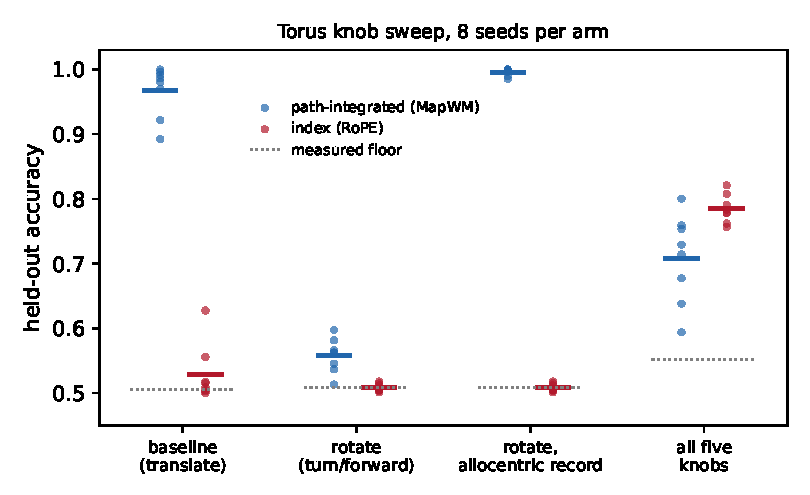
\includegraphics[width=0.72\linewidth]{figures/knob_sweep.pdf}
\caption{Per-seed accuracy for Table~\ref{tab:knob}. Dotted lines are each condition's measured floor;
bars are arm means. Generated by \texttt{figures/make\_knob\_sweep.py} from
\texttt{KNOB\_SWEEP\_n8.json}.}
\label{fig:knob}
\end{figure}

Rotation alone takes the position effect from $+0.438$ to $+0.050$, a reduction of $0.388$; all five knobs
combined take it to $-0.076$, a change of $-0.514$. The mechanism is supported by an intervention on the
action record alone: the same dynamics, recorded so that each token names a fixed displacement, restore the
effect to $+0.488$ against the baseline's $+0.438$ (no \mde\ recorded; trained at matched supervised events,
four times the baseline's batches). The recoding supplies an integrable input, not the target, but it removes the heading-to-displacement
computation from what is learned: the result shows that a fixed per-token increment cannot perform that
computation, not that a map can do without it. It requires the agent's heading to be known, which holds in
every simulator used here. % src: BASELINE_TABLE.md sec. I (D11); KNOB_SWEEP_n8.md

\subsection{Heading resolution}
\label{sec:c2-heading}

At 12 headings, with real-valued position, the allocentric record still separates the arms: every
path-integrated seed is above every index seed at every budget tried, the weakest path-integrated seed
scoring $0.661$ and the strongest index seed $0.555$ (floor 0.508--0.509; $n=3$ per budget, three
budgets). The size is not monotone in budget: $+0.264$ at 980 batches, $+0.383$ at 2000 and $+0.286$
at 4000, where two of three path-integrated seeds converged to worse losses and the index arm left the
floor. Accuracy tracks final training loss at $r=-0.996$ over the 18 runs, so arm-to-arm variation
here is convergence. The direction is an existence statement; the magnitude is exploratory.
% src: H12_BUDGET_CURVE.md, CONTINUOUS_ALLOC.md (D12)

\subsection{An external benchmark: MiniGrid}
\label{sec:c2-minigrid}

\paragraph{Commanded actions.} On MiniGrid DoorKey-16x16 with egocentric observations and the
environment's own turn-and-forward actions, the full $2\times2\times2$ factorial (encoding, position,
hierarchy; three layers, parameter-matched, $n=8$) puts index arms first: \arm{PoPE-Hier}
$0.955\pm0.003$ and \arm{PoPE-Flat} $0.953\pm0.003$ at $T=1024$, with the paper's \arm{MapWM-Flat}
last at $0.823\pm0.088$ (floor 0.490). The main effects at $T=1024$ are encoding $+0.076$, hierarchy
$+0.048$ and position $-0.021$; no sd was recorded for them, so they are directional. The arm means
are citable levels. This is the regime Section~\ref{sec:c2-knob} predicts: commanded rotation actions
make a fixed per-token increment misspecified. % src: MINIGRID_FULL_2X2X2.md, BASELINE_TABLE.md (D6)

\paragraph{Allocentric actions.} With actions recorded as realised grid displacement
(Table~\ref{tab:minigrid-allo}; one batch, $n=8$, 50 epochs), MapWM at $r=4$ beats the index arm on
every seed: \arm{Vanilla\_r4} minus \arm{RoPE} is $+0.034$ (\mde\ $0.014$, $8/8$) at $T=1024$. At the
paper's $r=2$ the contrast is $-0.010$ (\mde\ $0.056$, $4/8$), unmeasured. The effect is small, on a
benchmark where every arm is far above the floor; the claim is the sign conditioned on $r=4$, not its
size. An earlier three-seed factorial found the same sign flip at $r=2$ with effects of about 0.02,
compared across batches (Appendix~\ref{app:env}). % src: MINIGRID_EM.md (D8); MINIGRID_ALLOCENTRIC_2X2X2.md (D7)

\begin{table}[t]
\centering
\small
\captionsetup{font=footnotesize,skip=4pt}
\caption{Allocentric MiniGrid DoorKey-16x16 (actions recorded as realised displacement): held-out observation-prediction accuracy at $T=1024$, trained at $T=128$; $n=8$ per arm, one batch, floor 0.490. \arm{RoPE} = index position; \arm{Vanilla} = MapFormer-WM; \arm{VanillaEM} = MapFormer-EM, separate origins (discussed in Section~\ref{sec:c4-map}); \_r4 = bottleneck rank 4, else 2. Parameters 613,576--614,664 across the five arms (training logs). Contrast = arm minus \arm{RoPE}, paired by seed: delta (\mde, seeds with a positive difference); \mde\ = minimum detectable effect, $2.8\,\mathrm{sd}/\sqrt{n}$; detectable = beyond it; unmeasured = within it, not evidence of zero. Reading: MapWM beats the index arm on every seed only at $r=4$, by a small amount.}
\label{tab:minigrid-allo}
\begin{tabular}{@{}lccl@{}}
\toprule
arm & accuracy & worst seed & contrast with \arm{RoPE} \\
\midrule
\arm{RoPE} (index)       & $0.788\pm0.019$ & 0.754 & -- \\
\arm{Vanilla} ($r=2$)    & $0.778\pm0.045$ & 0.693 & $-0.010$ (\mde\ $0.056$, $4/8$), unmeasured \\
\arm{Vanilla\_r4}        & $0.822\pm0.015$ & 0.798 & $+0.034$ (\mde\ $0.014$, $8/8$), detectable \\
\arm{VanillaEM} ($r=2$)  & $0.763\pm0.081$ & 0.572 & $-0.026$ (\mde\ $0.087$), unmeasured \\
\arm{VanillaEM\_r4}      & $0.803\pm0.056$ & 0.666 & $+0.015$ (\mde\ $0.062$, $7/8$), unmeasured \\
\bottomrule
\end{tabular}
% src: MINIGRID_EM.md (D8); parameter counts from runs/minigrid_em/logs/*_s0.log
\end{table}

\subsection{MiniWorld: convergence, aliasing and map extent}
\label{sec:c2-miniworld}

MiniWorld's OneRoom environment is used as a continuous 3D geometry generator: location-keyed aliased
tokens are emitted on a fresh map per episode, and actions are recoded to the exact cell transition.

\paragraph{Convergence first.} At 100 epochs with linear decay, \arm{RoPE} never converged at grid 16
or above ($0/9$) and \arm{Vanilla} never at grid 8 ($0/3$), so an apparent crossover in grid size
tracked which arm had converged. At 400 epochs with warmup and cosine every arm is flat. There,
path integration is ahead of the index code at grid 32 ($+0.173$, $n=3$; extended below to $n=5$, where it is detectable) and both
arms solve grid 8 ($-0.010$, sd $0.007$, with \arm{RoPE} at $1.000$ on all three seeds). No regime was
found in which the index code is genuinely better. % src: POSITION_EFFECT_CONVERGED.md, CROSSOVER_CONVERGED.md (D19)

\paragraph{Aliasing does not drive the effect.} Holding the map at grid 32 and varying only the number
of observation types changes nothing but the labelling: label mass (50.4 scored events per trajectory)
and median revisit lag (33) are identical across conditions. The pre-registered aliasing hypothesis
predicted that the effect would collapse as aliasing fell. At 400 epochs every level meets outcome B's
numeric condition (effect above 0.150), but the $n_{\mathrm{obs}}=64$ and $256$ arms were not all converged
and the scripted verdict was withheld (``not all arms converged'', Table~\ref{tab:alias}). The falsification
therefore rests on the converged cells: $+0.178$ at $n_{\mathrm{obs}}=16$ ($n=5$, \mde\ $0.118$, all arms
flat) and, extended to 800 epochs, $+0.305$ at $n_{\mathrm{obs}}=256$ (sd $0.048$, \mde\ $0.077$, $3/3$,
exploratory) with every arm flat. No test of the difference between these two was run, and they differ in
budget and $n$. The post-hoc pooled reading of the next paragraph points the same way. The final losses of the two arms do not overlap at
$n_{\mathrm{obs}}=64$ and $256$, so this study measures ``optimises better'', not ``represents better at
equal fit''. % src: ALIASING_GATES.md, ALIASING_CONTROLLED.md verdict (D20); MINIWORLD_ENDPOINTS.md; VISITS_TEST.md

\begin{table}[t]
\centering
\small
\captionsetup{font=footnotesize,skip=4pt}
\caption{MiniWorld at fixed grid 32 (about 512 occupied cells), $T=512$, only the number of observation types $n_{\mathrm{obs}}$ varied: non-blank accuracy (scored cells whose answer is not blank) on a fresh map, path-integrated (MapFormer-WM) minus index, paired by seed. Floors are the non-blank marginals; $n$ = seeds per arm; sd = of paired differences; \mde\ = minimum detectable effect, $2.8\,\mathrm{sd}/\sqrt{n}$; flat = converged. Rows 1--3 are the 400-epoch study (scripted verdict withheld: not all arms converged); row 4 extends $n_{\mathrm{obs}}=256$ to 800 epochs. Reading: the effect does not shrink as aliasing falls; this rests on the two converged cells, which differ in budget and $n$, untested against each other.}
\label{tab:alias}
\begin{tabular}{@{}lcccccc@{}}
\toprule
$n_{\mathrm{obs}}$ & cells per token & floor & epochs & $n$ & effect & sd / \mde \\
\midrule
16  & 32 & 0.077 & 400 & 5 & $+0.178$ & $0.094$ / $0.118$; all arms flat \\
64  & 8  & 0.031 & 400 & 4 & $+0.310$ & $0.031$ / $0.043$; not all flat \\
256 & 2  & 0.013 & 400 & 5 & $+0.374$ & $0.046$ / $0.057$; not all flat \\
256 & 2  & 0.013 & 800 & 3 & $+0.305$ & $0.048$ / $0.077$; all flat (exploratory, $n=3$) \\
\bottomrule
\end{tabular}
% src: ALIASING_CONTROLLED.md (D20, rows 1-3); MINIWORLD_ENDPOINTS.md (row 4)
\end{table}

\paragraph{Map extent, an open threshold.} At matched aliasing (2 cells per token), pooling the
conditions available after the fact gives the pattern in Table~\ref{tab:extent}: flat at 32 and 128
occupied cells, and large at 512. Within a map size the effect moves by $0.005$ (grid 16) and $0.030$
(grid 32) as the number of prior visits per scored cell changes; across map sizes it moves by $0.285$.
One hypothesis is falsified outright: at a matched number of distinct cells visited, grid 32 at $T=128$
gives $+0.275$ where grid 8 at $T=512$ gives $-0.010$. The map-extent reading is a post-hoc pooled
analysis at $n=3$ per point; the pre-registered pairwise verdict was that prior visits and map extent
could not be separated. The two endpoints were trained at different budgets (800 and 400 epochs), and
the grid-16 point is a ceiling (the index arm scores $0.971$--$0.994$). The threshold between 128 and
512 occupied cells is therefore a boundary to test, not a finding. The MiniWorld run-to-run noise
floor of 0.150 was measured on mostly unconverged runs; both it and the paired \mde\ are given.
% src: VISITS_TEST.md (D21); MINIWORLD_ENDPOINTS.md; MINIWORLD_GATE_CONTROL.md (D17)

\begin{table}[t]
\centering
\small
\captionsetup{font=footnotesize,skip=4pt}
\caption{MiniWorld map extent at 2 cells per token (grid 8 at $n_{\mathrm{obs}}=16$ is 2 cells per token as well): non-blank accuracy on a fresh map, path-integrated minus index, paired by seed. $T$ = episode length; prior visits = mean earlier visits per scored cell; notes give index-arm accuracy and sd / \mde\ (minimum detectable effect) where recorded. $n=3$ per row, post-hoc pooling of runs at different budgets. Exploratory. Reading: flat at 32 and 128 occupied cells, large at 512; the threshold is a boundary to test, not a finding.}
\label{tab:extent}
\begin{tabular}{@{}cccccl@{}}
\toprule
grid & occupied cells & $T$ & prior visits & effect & note \\
\midrule
8  & 32  & 512  & 8.64 & $-0.010$ & both arms solve \\
16 & 128 & 512  & 4.61 & $+0.015$ & sd $0.013$, \mde\ $0.020$; index $0.971$--$0.994$ (ceiling) \\
16 & 128 & 1024 & 6.20 & $+0.010$ & index $0.987$ \\
32 & 512 & 128  & 1.95 & $+0.275$ & index $0.674$ \\
32 & 512 & 512  & 3.05 & $+0.305$ & sd $0.048$, \mde\ $0.077$; 800 epochs \\
\bottomrule
\end{tabular}
% src: VISITS_TEST.md pooled table (D21); MINIWORLD_ENDPOINTS.md (rows 2 and 5)
\end{table}

\subsection{What is not modelled}
\label{sec:c2-habitat}

In Habitat, measured with the simulator but with no model trained, 69--91\% of forward moves across
three scenes do not produce the commanded 0.25\,m displacement: the navigation mesh slides or blocks
the agent. Displacement there is continuous in magnitude as well as direction, which no experiment
here models. % src: HABITAT_BUILD.md (D13)

%======================================================================
\section{Claim 3: the increment must cancel, and cancel cleanly}
\label{sec:claim3}
%======================================================================

For the interval sum to measure net displacement, opposite actions must produce cancelling increments,
and the basis they live in must be well conditioned. Forcing the increment non-negative costs MapWM $0.363$
raw (\mde\ $0.025$) and $0.280$ at matched loss (\mde\ $0.061$) on the torus at $T=1024$ ($12/12$), and at
matched loss leaves no measurable gain over an index code (raw, the monotone arm stays ahead of it, $+0.213$,
\mde\ $0.097$); Selective RoPE's generator pays the same raw cost ($-0.355$ against MapWM's $-0.363$). The
paper's $r=2$ bottleneck learns a skewed basis, and $r=4$ adds $+0.085$ at $T=1024$ ($8/8$) for 384
parameters. The value of both depends on the task: on a counting task the same sign constraint costs
MapWM an unmeasured $-0.060$ and Selective RoPE's generator a small, detectable $-0.068$ (both raw); for that
generator, its raw torus cost minus its recency cost is detectable ($-0.287$). In the same batch single-origin
MapEM pays $-0.198$ raw on the counting task (\mde\ $0.155$), detectable ($-0.043$ at matched loss, \mde\ $0.051$,
unmeasured), and the difference between MapEM's and MapWM's costs is unmeasured ($-0.138$, \mde\ $0.181$). For
the two WM-type generators the constraint's cost is large on a map task and small on a counting task.
% src: SIGN_ABLATION.md (E11); MONOTONE_RESULTS.md; RANK_SWEEP.md (E1)

\subsection{Sign}
\label{sec:c3-sign}

\paragraph{Design.} Six arms, twelve seeds, one batch, torus recipe. The signed arm uses
$\Delta=W_{\mathrm{out}}W_{\mathrm{in}}x$; \arm{Abs\_r4} uses $|\Delta|$, the one-operation isolation;
\arm{Pos\_r4} and \arm{CARoPE\_r4} use the non-negative parameterisations of GRAPE's additive
path and CARoPE; \arm{Vanilla\_r4} is a construction control; \arm{RoPE} is the index code. All five
MapFormer arms have 204,757 parameters. The constraint holds after training (no negative increment in
the constrained checkpoints probed, seeds 0--2 of 12 per arm), and the construction control differs from the signed arm by $+0.000$,
$+0.006$ and $+0.006$ at the three lengths, unmeasured throughout. Rule 9 gives $r=-0.978$, $-0.856$
and $-0.729$ at $T=128$, 512 and 1024 over 72 runs. % src: SIGN_ABLATION.md, SIGN_PROBE.md (E11, E12)

\begin{table}[t]
\centering
\small
\captionsetup{font=footnotesize,skip=4pt}
\caption{Sign ablation, torus: accuracy predicting the observation at revisited cells of a held-out map, trained at $T=128$; mean $\pm$ sd, $n=12$ per arm, one batch, floor 0.506; final loss = arm mean. All but \arm{RoPE} are MapFormer-WM at $r=4$ with 204,757 parameters: \arm{Signed\_r4} = free-sign increment $\Delta$; \arm{Vanilla\_r4} = construction control; \arm{Abs\_r4} = $|\Delta|$; \arm{Pos\_r4} = softplus increment (GRAPE-style); \arm{CARoPE\_r4} = CARoPE's increment in $(0,1)$. \arm{RoPE} = index position. Reading: at training length the signed arm is at ceiling and the constraint's cost shows in the loss; accuracy contrasts are in Table~\ref{tab:sign-contrasts}.}
\label{tab:sign}
\begin{tabular}{@{}lcccc@{}}
\toprule
arm & $T=128$ & $T=512$ & $T=1024$ & final loss \\
\midrule
\arm{Signed\_r4}  & $1.000\pm0.000$ & $0.978\pm0.014$ & $0.922\pm0.027$ & 0.0002 \\
\arm{Vanilla\_r4} & $1.000\pm0.000$ & $0.984\pm0.009$ & $0.927\pm0.015$ & 0.0002 \\
\arm{Abs\_r4}     & $0.946\pm0.070$ & $0.675\pm0.040$ & $0.558\pm0.027$ & 0.1708 \\
\arm{Pos\_r4}     & $0.977\pm0.035$ & $0.798\pm0.080$ & $0.584\pm0.080$ & 0.0676 \\
\arm{CARoPE\_r4}  & $0.900\pm0.138$ & $0.809\pm0.133$ & $0.645\pm0.090$ & 0.2929 \\
\arm{RoPE}        & $0.799\pm0.018$ & $0.449\pm0.083$ & $0.345\pm0.118$ & 0.7844 \\
\bottomrule
\end{tabular}
% src: SIGN_ABLATION.md (E11)
\end{table}

\begin{table}[t]
\centering
\small
\captionsetup{font=footnotesize,skip=4pt}
\caption{Sign ablation contrasts on the torus (arms as in Table~\ref{tab:sign}: \arm{Signed} free sign; \arm{Abs}, \arm{Pos}, \arm{CARoPE} non-negative; \arm{RoPE} index), first-named minus second, paired by seed, $n=12$, trained at $T=128$. Main value: loss-matched, i.e.\ compared at equal final training loss by a regression pooled over the six arms (verdicts depend on the pool); raw difference in parentheses where recorded. \mde\ = minimum detectable effect, $2.8\,\mathrm{sd}/\sqrt{n}$; detectable = beyond it; unmeasured = within it, not evidence of zero. Rule 9, $r(\text{loss},\text{accuracy})$: $-0.978$, $-0.856$, $-0.729$ at the three lengths. Reading: at matched loss the monotone arm is worse than signed by 0.215 and 0.280 beyond training length and beats the index code nowhere; raw it stays above \arm{RoPE}, which trains to a much higher loss.}
\label{tab:sign-contrasts}
\resizebox{\linewidth}{!}{%
\begin{tabular}{@{}lccc@{}}
\toprule
contrast & $T=128$ & $T=512$ & $T=1024$ \\
\midrule
\arm{Abs} $-$ \arm{Signed}    & $-0.006$ (\mde\ $0.018$) & $-0.215$ (\mde\ $0.055$; raw $-0.303$) & $-0.280$ (\mde\ $0.061$; raw $-0.363$) \\
\arm{Pos} $-$ \arm{Signed}    & $-0.004$ (\mde\ $0.010$), unmeasured & $-0.145$, detectable & $-0.305$, detectable \\
\arm{CARoPE} $-$ \arm{Signed} & $-0.017$ (\mde\ $0.023$), unmeasured & $-0.018$, unmeasured & $-0.134$ (\mde\ $0.118$), detectable \\
\arm{Signed} $-$ \arm{RoPE}   & $-0.021$ (\mde\ $0.013$), detectable & $+0.123$ (\mde\ $0.075$) & $+0.195$ (\mde\ $0.107$) \\
\arm{Abs} $-$ \arm{RoPE}      & $-0.028$ (\mde\ $0.025$; raw $+0.146$, \mde\ $0.055$) & $-0.092$ (\mde\ $0.103$; raw $+0.226$, \mde\ $0.059$) & $-0.085$ (\mde\ $0.140$; raw $+0.213$, \mde\ $0.097$) \\
\bottomrule
\end{tabular}}
% src: SIGN_ABLATION.md (E11)
\end{table}

\paragraph{Result.} Tables~\ref{tab:sign} and~\ref{tab:sign-contrasts}. At matched loss, the monotone
arm is worse than the signed arm by $0.215$ at $T=512$ and $0.280$ at $T=1024$, on $12/12$ seeds at
both. At matched loss, signed path integration beats the index code by $+0.123$ and $+0.195$, and the
monotone arm beats it nowhere (\arm{Abs} $-$ \arm{RoPE} is unmeasured at $T=512$ and 1024 and detectably
negative at $T=128$; so is \arm{Signed} $-$ \arm{RoPE} at $T=128$, $-0.021$). On raw accuracy the monotone
arm is detectably above the index code at every length ($+0.146$, $+0.226$ and $+0.213$ at $T=128$, 512 and
1024, \mde\ $0.055$, $0.059$ and $0.097$), because \arm{RoPE} trains to a much higher loss. At matched loss,
the measured value of a content-dependent phase over an index code on this task therefore requires the
sign. % src: SIGN_ABLATION.md (E11), contrast tables and sec. 4

At $T=128$ the accuracy discriminator could not show a deficit: the signed arm sits at
$1.000\pm0.000$. The pre-registered hypothesis asked for a training-length accuracy deficit in that
ceiling cell, a design error recorded before any result was read. The training-length effect is in the
loss: every constrained arm has a higher final training loss than the signed arm on $12/12$ seeds
(\arm{Abs} $+0.1706$, \arm{Pos} $+0.0674$, \arm{CARoPE} $+0.2927$). The \arm{Pos} and \arm{CARoPE}
arms carry an initialisation confound (they start close to RoPE, the signed arms close to NoPE).
% src: SIGN_ABLATION.md, SIGN_ABLATION_PREREG.md (E11)

\paragraph{The learned code.} The opposition score $\|D(+a)+D(-a)\|/\overline{\|D\|}$ is 0 when opposite
actions cancel and 2 when they are identical. It is $0.125$ and $0.106$ (two axes; seeds 0--2) for the signed arm
and $0.128$ and $0.130$ for the construction control, against $1.849$/$1.855$ for \arm{Abs},
$1.905$/$1.885$ for \arm{Pos} and $1.981$/$1.977$ for \arm{CARoPE}. A monotone code cannot reach 0 by
construction; the informative part is that the signed arm does reach about 0.1. Cancellation chooses
what the accumulator measures: signed increments give net displacement, a map; monotone increments give
path length, a clock. % src: SIGN_PROBE.md (E12)

\paragraph{A second generator.} A pre-registered batch (96 runs, one batch, 12 seeds per arm) repeated
the constraint on Selective RoPE's generator (\arm{SRoPEGen}: gate, causal convolution, no rank
bottleneck). On the torus, \arm{SRoPEGen} scores $1.000$, $0.984$ and $0.899$ at $T=128$, 512 and
1024 and its monotone twin $0.925$, $0.638$ and $0.545$. The raw cost at $T=1024$ is $-0.355$ (\mde\
$0.046$, $0/12$), against MapWM's stored raw cost of $-0.363$ (\mde\ $0.025$); the difference between the
two generators' costs is $+0.009$ (\mde\ $0.052$), unmeasured. The raw sign cost on navigation is therefore
not specific to MapFormer's generator. The registered loss-matched form (Q1) was falsified as
registered: its loss-matching pool contained only the two \arm{SRoPEGen} arms, whose final losses do not
overlap ($0.0002$--$0.0006$ against $0.20$--$0.47$), so the fit absorbed the effect by construction and
returned $-0.056$ (\mde\ $0.083$). In an exploratory eight-arm pool that includes the six stored sign
arms, the loss-matched cost is $-0.188$ (\mde\ $0.059$, $0/12$). % src: MONOTONE_RESULTS.md

\paragraph{Prior art.} The sign axis and the parity theorem are due to \citet{sarrof2024expressive} and
\citet{grazzi2025unlocking}, and were carried into content-dependent rotation in attention by
\citet{movahedi2026srope}. CARoPE, GRAPE's additive path and CoPE are non-negative. What is new here is
the navigation regime and the one-operation isolation at identical parameter count.

\subsection{Rank}
\label{sec:c3-rank}

\paragraph{The sweep.} Only $r$ varies across five arms, eight seeds each, one batch, torus recipe
(Table~\ref{tab:rank}, Figure~\ref{fig:rank}). Against $r=2$, $r=4$ adds $+0.085$ at $T=1024$ (t
$3.57$, $8/8$) and $+0.038$ at $T=512$. The gain is a step: $r=8$, 16 and 32 give $+0.091$, $+0.079$ and
$+0.095$ at $T=1024$, all $8/8$. $r=4$ also cuts the $T=1024$ seed sd from $0.064$ to $0.012$, which
matters because sd sets every \mde. It costs 384 parameters; Selective RoPE's gate arm (sigmoid gate plus a readout swap) reached a
similar $+0.086$ at $T=1024$ for $8{,}193$ parameters, an effect that cannot be attributed to the gate (Appendix~\ref{app:rank}). The pre-registered
branch ``accuracy rises with $r$'' fired. $r=1$ and $r=3$ were not run. % src: RANK_SWEEP.md (E1); SELECTIVE_ROPE.md (E15)

\begin{table}[t]
\centering
\small
\captionsetup{font=footnotesize,skip=4pt}
\caption{Rank sweep on MapFormer-WM, torus: accuracy predicting the observation at revisited cells of a held-out map, trained at $T=128$; only the bottleneck rank $r$ varies (parameters in the first column); mean $\pm$ sd, $n=8$ per arm, one batch, floor 0.506. Last column: minus $r=2$ at $T=1024$, paired by seed ($t$ statistic where recorded; seeds with a positive difference). Reading: $r=4$ adds $+0.085$ at $T=1024$ for 384 parameters and cuts seed sd from 0.064 to 0.012; the gain is a step.}
\label{tab:rank}
\begin{tabular}{@{}lcccc@{}}
\toprule
arm (parameters) & $T=128$ & $T=512$ & $T=1024$ & vs $r=2$ at $T=1024$ \\
\midrule
$r=2$ (204,373)  & $0.993\pm0.017$ & $0.944\pm0.028$ & $0.834\pm0.064$ & -- \\
$r=4$ (204,757)  & $1.000\pm0.000$ & $0.982\pm0.005$ & $0.919\pm0.012$ & $+0.085$ (t $3.57$, $8/8$) \\
$r=8$ (205,525)  & $1.000\pm0.000$ & $0.981\pm0.018$ & $0.925\pm0.033$ & $+0.091$ ($8/8$) \\
$r=16$ (207,061) & $1.000\pm0.000$ & $0.972\pm0.015$ & $0.913\pm0.018$ & $+0.079$ ($8/8$) \\
$r=32$ (210,133) & $1.000\pm0.000$ & $0.982\pm0.010$ & $0.928\pm0.021$ & $+0.095$ ($8/8$) \\
\bottomrule
\end{tabular}
% src: RANK_SWEEP.md (E1)
\end{table}

\begin{figure}[t]
\centering
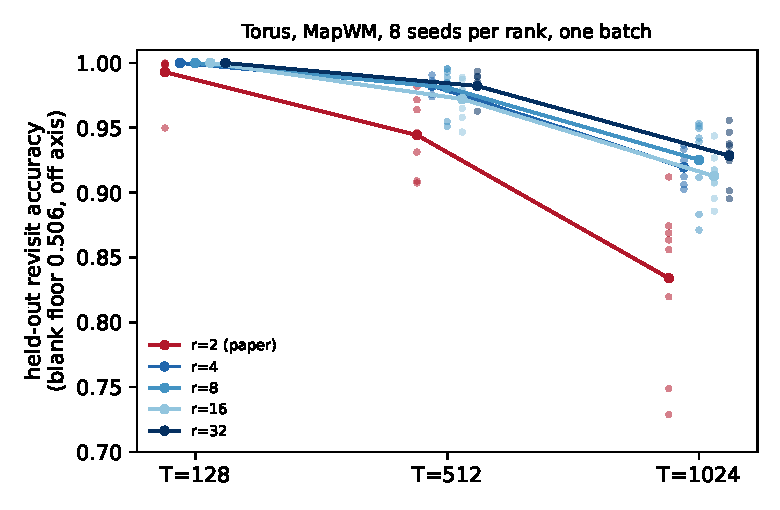
\includegraphics[width=0.66\linewidth]{figures/rank_sweep.pdf}
\caption{Per-seed held-out accuracy for Table~\ref{tab:rank}; lines join arm means. Generated by
\texttt{figures/make\_rank\_sweep.py} from \texttt{RANK\_SWEEP.json}.}
\label{fig:rank}
\end{figure}

\paragraph{What $r=2$ learns.} Given more than two dimensions, the model still places its actions in a
two-dimensional plane (plane energy $1.0000$ at $r=4$ and $0.9996$ at $r=32$), so the learned codes are
two-dimensional, as the paper's argument expects ($r=1$ was not run). What fails at $r=2$ is the basis: opposite actions fail to cancel by half
the action scale (opposition $0.4950$ against $0.0922$ at $r=4$), and north and east are nearly parallel
($|\cos| = 0.7833$ against $0.1754$). This is a description of the learned codes on eight seeds; the
causal route from skew to accuracy is not tested. The paper's own reported limitation, non-orthogonal
actions ($0.779$ in Table~\ref{tab:fig4}), falls to $0.174$ at $r=4$ with no regulariser.
% src: ACTION_GEOMETRY.md (E2); PAPER_FIG4_REPRO.md (E5)

\paragraph{Scope.} The rank result is conditional.
\begin{itemize}
\item \textbf{MapPoPE.} $r=4$ against $r=2$ on MapPoPE is $+0.019$ at $T=1024$ ($5/8$; loss-matched
$+0.015$), unmeasured. PoPE has 64 frequency channels per head to MapWM's 32, which may explain it; that reason
is untested. ``Use $r=4$'' is a MapWM-family recommendation. % src: MAPPOPE_R4_RESULTS.md (E8)
\item \textbf{Match-Query.} Rank alone adds $+0.005$ (\mde\ $0.091$), unmeasured; with a four-pass loop
it adds $+0.154$ (\mde\ $0.084$, $8/8$), paired on a task where pairing is unreliable (Section~\ref{sec:c5-loop}). % src: MQ_RANK_2X2.md (C13)
\item \textbf{MiniGrid.} The allocentric path-integration gain exists only at $r=4$
(Section~\ref{sec:c2-minigrid}). % src: MINIGRID_EM.md (D8)
\end{itemize}

\paragraph{Not packing geometry.} If $r=2$'s deficit were a packing effect of $D$ displacement axes into
$r$ dimensions, it should grow with $D$, which was proposed as an account of the paper's 5D collapse.
On a $D$-dimensional torus ($D=2,3,5$; eight seeds; gates at chance) $r=2$ posts its best score at $D=5$
($0.896\pm0.076$) and its deficit against the best higher rank is $+0.110$, $+0.153$ and $+0.055$ at
$D=2$, 3 and 5 at $T=512$, not growing with $D$. Two of three pre-registered falsifiers fired and the
account is withdrawn; the paper's own 5D run used $r=D$ (App.~D.1). That the gap is an optimisation effect rests on
one independent detectable cell, $r=D+2$ minus $r=D$ at $D=5$ ($+0.073$, t $3.35$, $8/8$), and is exploratory.
% src: DXR_RANK_THRESHOLD.md, ND_GATES.md (E7, D26); mapformer_math.tex (r=D+2 minus r=D table); papers/txt/mapformer.txt App. D.1 (r=D)

\subsection{The task sets the value}
\label{sec:c3-task}

\paragraph{Recency.} The same arms trained on $k$-back retrieval with uncounted filler
(Table~\ref{tab:recency}; eight seeds, one batch) give a different picture. $T=1024$ is at ceiling for
two arms, so the registered comparison is at $T=2048$. There, \arm{Abs} minus \arm{Signed} is $-0.052$
raw (\mde\ $0.105$) and $+0.016$ loss-matched (\mde\ $0.046$), and the mean of the three monotone arms
minus \arm{Signed}, the registered primary, is $-0.004$ raw (\mde\ $0.055$) and $+0.026$ loss-matched
(\mde\ $0.027$): all unmeasured. % src: RECENCY_RESULTS.md (E24)

\begin{table}[t]
\centering
\small
\captionsetup{font=footnotesize,skip=4pt}
\caption{Recency: return the $k$-th most recent symbol ($k_{\max}=64$) past uncounted filler ($p_{\mathrm{filler}}=0.5$); retrieval accuracy on held-out episodes, trained at $T=1024$; mean $\pm$ sd, $n=8$ per arm, one batch; final loss = final training loss. Sign arms (MapFormer-WM, $r=4$) as in Table~\ref{tab:sign}: \arm{Signed\_r4} free sign, the others non-negative. \arm{RoPE}, \arm{PlainFlat} = index position. Chance 0.0625; most-recent floor 0.0771. Reading: index arms fail, path-integrated arms succeed, and the non-negative constraint's cost is unmeasured here.}
\label{tab:recency}
\begin{tabular}{@{}lccc@{}}
\toprule
arm & final loss & $T=1024$ & $T=2048$ \\
\midrule
\arm{Signed\_r4}  & 0.025 & $1.000\pm0.000$ & $0.940\pm0.050$ \\
\arm{CARoPE\_r4}  & 0.020 & $1.000\pm0.000$ & $0.973\pm0.028$ \\
\arm{Pos\_r4}     & 0.061 & $0.979\pm0.041$ & $0.947\pm0.069$ \\
\arm{Abs\_r4}     & 0.110 & $0.961\pm0.068$ & $0.889\pm0.126$ \\
\arm{RoPE}        & 2.150 & $0.234\pm0.025$ & $0.234\pm0.011$ \\
\arm{PlainFlat}   & 2.143 & $0.236\pm0.019$ & $0.233\pm0.009$ \\
\bottomrule
\end{tabular}
% src: RECENCY_RESULTS.md (E24)
\end{table}

The pre-registered MONOTONE batch measured the recency half again, in one batch with the torus half for
the second generator. On recency at $T=1024$, the monotone constraint costs MapWM $-0.060$ (\mde\
$0.084$, $1/12$), unmeasured, and costs \arm{SRoPEGen} $-0.068$ (\mde\ $0.054$, $2/12$), a small
detectable amount; at $T=2048$, in contrasts not registered (exploratory), both are unmeasured ($-0.015$, \mde\ $0.097$; $-0.052$, \mde\ $0.076$).
For \arm{SRoPEGen}, the torus cost minus the recency cost is $-0.287$ (se $0.025$, \mde\ $0.071$),
detectable. The accurate form of the crossover is therefore that, for the two WM-type generators, the sign
constraint is large on a map task and small, but not always unmeasured, on a counting task; single-origin MapEM
pays a detectable $-0.198$ there (Section~\ref{sec:c4-search}). % src: MONOTONE_RESULTS.md (P2, Q2, Q3, exploratory rows)

\paragraph{What the free arm learns.} The unconstrained arm learns a different accumulator on each
task. The growth exponent $\alpha$ of the accumulator's range, $\mathrm{range}(S)\sim T^{\alpha}$, is
$0.591\pm0.028$ on the torus and $0.967\pm0.009$ on recency for \arm{Signed\_r4}, while the constrained
arms sit near 1 on both (\arm{Abs\_r4} $1.010$ and $0.976$). % src: RECENCY_H2.md (E25)

\paragraph{How it counts, by intervention.} Eval-only interventions on the trained signed arm
(Table~\ref{tab:gate-ablation}) show that a content gate is most of the counting mechanism. Removing
filler increments costs $-0.0003$. Replacing $\Delta$ with a magnitude-matched constant on content tokens
only scores $0.7826$; the same constant on every token scores $0.1886$: $+0.594$ on $8/8$ seeds. An
``equalize'' condition that looked decisive ($0.0855$) is confounded, because a control that changes only
the scale of $\theta$ collapses as hard ($0.1096$); the magnitude-matched pair was added after that
control failed and is labelled as not pre-registered. Gate strength does not predict accuracy near
ceiling ($r=-0.34$). That position should count only selected tokens is CoPE's mechanism; that an
unconstrained MapFormer discovers such a gate is the new observation. % src: RECENCY_GATE_ABLATION.md (E26)

\begin{table}[t]
\centering
\small
\captionsetup{font=footnotesize,skip=4pt}
\caption{Recency gate ablation: eval-only interventions on the increments $\Delta$ of trained \arm{Signed\_r4} (MapFormer-WM), $T=1024$, $n=8$; accuracy is the seed mean ($\pm$ sd where recorded). Content tokens are counted, filler is not. Chance 0.0625; index arms score 0.234. \texttt{scale\_match} is the control for \texttt{equalize}; the \texttt{uniform} pair is magnitude-matched and not pre-registered. Reading: a content gate is most of the counting mechanism ($+0.594$, $8/8$), and \texttt{equalize} is confounded.}
\label{tab:gate-ablation}
\begin{tabular}{@{}llc@{}}
\toprule
condition & what it does & accuracy \\
\midrule
none & -- & 1.0000 \\
zero\_filler & filler increments set to zero & 0.9997 \\
equalize & filler increments set to the mean content increment & 0.0855 \\
scale\_match & only the scale of $\theta$ changed (control) & 0.1096 \\
uniform\_content & magnitude-matched constant on content tokens & $0.7826\pm0.1150$ \\
uniform\_all & the same constant on every token & $0.1886\pm0.0248$ \\
zero\_content & content increments set to zero & 0.0680 \\
zero\_query & query increments set to zero & $0.8232\pm0.0797$ \\
\bottomrule
\end{tabular}
% src: RECENCY_GATE_ABLATION.md (E26)
\end{table}

\paragraph{Recency does not need a clock.} A signed accumulator can do $k$-back without counting upward.
If symbols carry $\Delta=(1,0)$ and the query token for offset $k$ carries $\Delta=(-(k-1),0)$, the prefix
sum rewinds the count at the query and the retrieval offset is zero for every query; a single-origin
kernel then selects the answer on 1423/1423, 1417/1417 and 1415/1415 queries in three draws.
Section~\ref{sec:claim4} shows the full model can hold this solution. The recency half of the crossover
shows that for MapWM a monotone increment is cheap there, not that it is required. % src: AUDIT_2026-09-10.md #2 (F2)

\subsection{One description, two severities}
\label{sec:c3-alpha}

Across four torus arms from two batches, $\alpha$ is $0.518$ (\arm{Signed\_r4}), $0.524$
(\arm{Vanilla\_r4}), $0.619$ ($r=2$) and $0.943$ (\arm{Abs\_r4}), and $r(\text{opposition},\alpha)=+0.9995$.
Sign and rank are then one finding at two severities: the monotone code cannot cancel at all, the $r=2$
code cancels badly. This is exploratory (four points, correlational), and $\alpha$ is a statistic fitted
to trained models, nearly collinear with the simpler opposition score, not a parameter that can be
varied. Two analyses give different torus exponents for \arm{Signed\_r4} ($0.518$ here, $0.591$ in the
recency comparison); each is quoted only beside its own comparison. % src: LOCALISATION.md P3 (E13); RECENCY_H2.md (E25)

The route from a growing accumulator to failure beyond training length is not established. The one
account imported for it, that low-frequency channels never complete a cycle at training length and are
read at unseen phases later, predicts that ablating those channels costs less out of distribution. It
costs more: ablating the 32 lowest-frequency of its 64 channels (2 heads $\times$ 32) of \arm{Signed\_r4} costs $-0.001$ at $T=128$ and
$-0.139\pm0.092$ at $T=1024$ (Section~\ref{sec:length}). % src: LOCALISATION.md P2 (E13)

%======================================================================
\section{Claim 4: a shared kernel is representable but harder to find}
\label{sec:claim4}
%======================================================================

MapEM factorises where from what completely: one position kernel is shared by every query--key pair.
On map tasks no detectable difference from MapWM was found once its initialisation is fixed, including
beyond the training length on MiniGrid. On varying-offset recency, single-origin
MapEM trails MapWM by $0.375$ (\mde\ $0.154$, $0/8$). The gap is not in what the model can represent: the
solution installed and frozen scores $1.000$ on $8/8$ seeds, and installed at training scale with a
content leak closed it is held at $1.000$ on $8/8$. From scratch MapEM finds the solution per query
token, in wrapped form, and a single shared offset is found on $7/8$ seeds. At a fixed budget, fewer
offsets are better ($+0.665$, \mde\ $0.213$, $8/8$). Per-pair position origins add $+0.215$ over single-origin MapEM at
$n=48$, split between pathway capacity ($+0.124$) and per-pair freedom ($+0.091$), and only the freedom
changes the mechanism (per-token rewind share $0.948\to0.189$). Every recency contrast in this section is a
contrast of fit, with $r(\text{loss},\text{accuracy})$ between $-0.936$ and $-0.987$; the
``search, not representation'' reading rests on the existence and holding constructions, not on
loss-matching.
% src: RECENCY_EM_RESULTS.md (F1); WARM_RESULTS.md (F9); NOLEAK_RESULTS.md (F11); SEARCH_RESULTS.md (F12, F14);
% src: SPREAD2_RESULTS.md (F16); PAIRSPLIT_RESULTS.md (F19); PAIRCONST_RESULTS.md (F18); D5_RESULTS.md, MONOTONE_RESULTS.md (r range)

\subsection{Two ways to compose where and what}
\label{sec:c4-compose}

Section~\ref{sec:background} set out the algebra: MapEM's $A_X\odot A_P$ is TEM's conjunction with one
kernel for every pair, up to a sign gauge; MapWM's kernel has per-pair amplitudes and phases. A probe of
the circular standard deviation of the kernel phase across 29,056 query--key pairs per model confirms the
parameterisation in trained recency models: $1.947$ for trained MapWM (seeds $1.83$--$2.08$; $2.722$
untrained), exactly $0.000$ for both MapEM forms, against a uniform null of $3.267$. Single-origin MapEM
keeps 25 of 64 frequency blocks alive; separate-origin MapEM all 64. The only reading licensed is that
MapWM can reshape its kernel per pair and MapEM cannot. Training reduces MapWM's spread, so the probe does
not show that MapWM's advantage comes from reshaping. % src: EM_WM_THEORY.md 1b (F4)

\subsection{Map tasks}
\label{sec:c4-map}

\paragraph{No detectable difference once initialisation is fixed.} On allocentric MiniGrid, single-origin MapEM at $r=4$ minus
MapWM at $r=4$ is $+0.0012$ ($T=512$, $4/8$) and $+0.0035$ ($T=1024$, $6/8$), unmeasured (no \mde\ was
recorded); its worst-to-second-worst seed gap is $0.002$, against $0.137$ for the paper's separate-origin
$r=2$ form. On the torus vocabulary sweep at $n_{\mathrm{obs}}=256$, the same contrast is $+0.0597$ (\mde\
$0.169$), unmeasured, all of it one collapsed \arm{Vanilla\_r4} seed; with each arm's worst seed dropped it is
$+0.0000$. Neither contrast is detectable.
% src: MINIGRID_EM_FIX.md (F23); VOCAB_EM.md (F21)

\paragraph{The origin design is task-dependent.} The paper's separate $q_0,k_0$ is worse than a single
$p_0$ on map tasks: on the torus recipe separate minus single is $-0.154$ (\mde\ $0.130$, $0/8$) at
$T=1024$, and on the paper task and Match-Query it is worse at $n=3$ (Section~\ref{sec:repro}). On
varying-offset recency it is directionally better: $+0.128$ (\mde\ $0.108$, $17/24$) pooled over 24
seeds, but $+0.073$ (\mde\ $0.130$, $9/16$) on the 16 fresh seeds alone, unmeasured.
% src: DOF_RESULTS.md (F6); D5_RESULTS.md (F7); PAPER_TASK_ACCURACY.md, MATCH_QUERY_EM.md (A8)

\paragraph{Length on the paper task.} On the paper's OOD-s condition extended to longer episodes, a
pre-registered 50-epoch rerun found MapEM degrading more slowly than MapWM (Table~\ref{tab:papertask-em}).
Floor-normalised, MapEM minus MapWM is $+0.067$ (\mde\ $0.168$) at $l=512$, $+0.186$ (\mde\ $0.185$,
$8/8$) at $l=1024$ and $+0.287$ (\mde\ $0.194$, $8/8$) at $l=2048$. Rule 9 gives $r=-0.461$, so this is not
simply a loss gap. The pre-registered convergence gate (every arm at IID $\ge0.99$) failed, with MapWM at $0.968$
and MapEM at $0.985$, so the registered verdict is not read; the numbers are exploratory. The effect is
monotone in length, the axis of Section~\ref{sec:length}, and it does not support ``a shared kernel is
better when the offset is fixed'': other fixed-offset tasks show no detectable difference. % src: PAPERTASK_RESULTS.md, PAPER_OOD_RERUN.md (A5, F20)

\begin{table}[t]
\centering
\small
\captionsetup{font=footnotesize,skip=4pt}
\caption{Paper task, extended OOD-s condition (larger map, $p_{\mathrm{empty}}=0.8$) at episode length $l$, 50-epoch rerun, $n=8$ per arm, one batch: accuracy predicting the observation at revisited cells of a held-out map, mean $\pm$ sd (floors 0.799--0.802 at $p_{\mathrm{empty}}=0.8$). \arm{Vanilla} = MapFormer-WM; \arm{VanillaEM\_P0} = MapFormer-EM, one origin; \arm{MapPoPE-Flat} = PoPE magnitude with MapFormer's phase. Contrasts: floor-normalised (fraction of the range above floor), paired by seed; \mde\ = minimum detectable effect, $2.8\,\mathrm{sd}/\sqrt{n}$. The pre-registered convergence gate failed; exploratory. Reading: MapEM degrades more slowly with length than MapWM.}
\label{tab:papertask-em}
\begin{tabular}{@{}lccc@{}}
\toprule
 & $l=512$ & $l=1024$ & $l=2048$ \\
\midrule
\arm{Vanilla} (MapWM)          & $0.964\pm0.029$ & $0.927\pm0.034$ & $0.886\pm0.035$ \\
\arm{VanillaEM\_P0} (MapEM)    & $0.978\pm0.015$ & $0.964\pm0.016$ & $0.942\pm0.024$ \\
\arm{MapPoPE-Flat}             & $0.991\pm0.003$ & $0.978\pm0.004$ & $0.963\pm0.005$ \\
\midrule
MapEM $-$ MapWM, normalised    & $+0.067$ (\mde\ $0.168$) & $+0.186$ (\mde\ $0.185$) & $+0.287$ (\mde\ $0.194$) \\
MapPoPE $-$ MapEM, normalised  & $+0.066$ (\mde\ $0.079$) & $+0.073$ (\mde\ $0.090$) & $+0.102$ (\mde\ $0.128$) \\
\bottomrule
\end{tabular}
% src: PAPER_OOD_RERUN.md; PAPERTASK_RESULTS.md (A5, F20)
\end{table}

\subsection{The recency gap}
\label{sec:c4-gap}

\citet{whittington2025tale} predicts that episodic-memory models learn faster than working-memory models
except on N-back. On varying-$k$ recency (eight seeds per arm, one batch, recency recipe;
Table~\ref{tab:recency-em}), MapWM reaches training loss below 0.5 on $8/8$ seeds, single-origin MapEM on
$0/8$ and separate-origin MapEM on $1/8$, so the registered prediction that EM is not faster held.
Single-origin MapEM minus MapWM is $-0.375$ (sd $0.156$, \mde\ $0.154$, $0/8$) at $T=1024$ and $-0.437$ at
$T=2048$; separate-origin minus MapWM is $-0.137$ (\mde\ $0.106$, $1/8$). The deficit grows with $k$: at
$k=64$ MapWM scores $0.97$, separate-origin MapEM $0.73$ and single-origin MapEM $0.37$. Single-origin
MapEM is well above chance ($0.600$ against $0.0625$). % src: RECENCY_EM_RESULTS.md, AUDIT_2026-09-10.md #9 (F1)

\begin{table}[t]
\centering
\small
\captionsetup{font=footnotesize,skip=4pt}
\caption{Varying-$k$ recency (return the $k$-th most recent symbol): retrieval accuracy on held-out episodes, trained at $T=1024$, mean $\pm$ sd, $n=8$ per arm, one batch. \arm{Vanilla\_r4} = MapFormer-WM; \arm{VanillaEM\_r4} = MapFormer-EM, separate origins; \arm{VanillaEM\_P0\_r4} = MapFormer-EM, one origin. Final loss = range over seeds; worst = worst seed at $T=1024$; last column = seeds reaching training loss $<0.5$ (median epoch). Chance 0.0625, most-recent floor 0.0771. Reading: at a shared budget single-origin MapEM trails MapWM by 0.375 at $T=1024$, separate-origin by 0.137.}
\label{tab:recency-em}
\begin{tabular}{@{}lccccc@{}}
\toprule
arm & final loss & $T=1024$ & $T=2048$ & worst & loss $<0.5$ \\
\midrule
\arm{Vanilla\_r4} (MapWM)           & 0.008--0.380 & $0.975\pm0.072$ & $0.947\pm0.078$ & 0.797 & $8/8$ (median ep.\ 70.5) \\
\arm{VanillaEM\_r4} (separate)      & 0.430--1.136 & $0.837\pm0.081$ & $0.728\pm0.106$ & 0.689 & $1/8$ \\
\arm{VanillaEM\_P0\_r4} (single)    & 0.924--1.885 & $0.600\pm0.126$ & $0.510\pm0.111$ & 0.365 & $0/8$ \\
\bottomrule
\end{tabular}
% src: RECENCY_EM_RESULTS.md, AUDIT_2026-09-10.md #9 (F1)
\end{table}

The varying-$k$ task is not \citet{whittington2025tale}'s N-back, which has a fixed $N$ and no filler; the
fixed-$k$ condition of Section~\ref{sec:c4-search} is the analogue, and there MapEM reached training loss below
0.5 in a median 54 epochs against MapWM's 99 (descriptive; no inferential contrast).
MapWM at four times the budget was not run, so $-0.375$ is a comparison at a shared budget and says
nothing about asymptotic ability. % src: EM_WM_STATE.md Sec. 1 (F1, F27); SPREAD_RESULTS.md caveat (F15)

\subsection{Existence and holdability}
\label{sec:c4-ladder}

Section~\ref{sec:c3-task} gave a kernel-level construction that solves recency. Table~\ref{tab:ladder}
tests it in the full one-layer model, one rung at a time.

\begin{table}[t]
\centering
\small
\captionsetup{font=footnotesize,skip=4pt}
\caption{The existence and holdability ladder for single-origin MapEM on recency (retrieval accuracy, trained at $T=1024$), $n=8$ per arm (seeds 0--7). ``Install'' writes the rewind code (the query's increment undoes the count, so the retrieval offset is zero) into the position pathway, frozen or trainable; ``scale'' is the weight scale at which it is written; ``leak closed'' holds the content columns of $W_{\mathrm{in}}$ at zero. $T=2048$ values are means; the last column counts seeds at $\ge0.95$, the registered readout. Reading: the solution is represented exactly, and held at 8$\times$ scale with the leak closed.}
\label{tab:ladder}
\begin{tabular}{@{}lccc@{}}
\toprule
arm & $T=1024$ & $T=2048$ & seeds $\ge0.95$ \\
\midrule
from scratch (\arm{VanillaEM\_P0\_r4})          & $0.600\pm0.126$ & -- & -- \\
installed, frozen                                & $1.000\pm0.000$ & $1.000\pm0.000$ & $8/8$ \\
installed at scale 1/64, trainable               & $0.642\pm0.266$ & 0.582 & $0/8$ \\
installed at scale 1/64, trainable, leak closed  & $0.784\pm0.281$ & 0.709 & $3/8$ \\
installed at scale 1/8 (8$\times$), trainable    & $0.941\pm0.063$ & 0.895 & $4/8$ \\
installed at 8$\times$, trainable, leak closed   & $1.000\pm0.000$ & 0.991 & $8/8$ \\
MapWM (\arm{Vanilla\_r4})                        & $0.975\pm0.072$ & -- & -- \\
\bottomrule
\end{tabular}
% src: WARM_RESULTS.md (F9); UNFREEZE_RESULTS.md (F10); NOLEAK_RESULTS.md (F11)
\end{table}

\paragraph{Existence.} With the rewind installed in the position pathway and frozen, and the content
branch learned from random initialisation, single-origin MapEM scores $1.000\pm0.000$ on $8/8$ seeds at
$T=1024$ and $T=2048$, at every $k$ from 1 to 64. Frozen minus from-scratch is $+0.400$ (\mde\ $0.125$,
$8/8$); frozen minus MapWM is $+0.025$ (\mde\ $0.071$), unmeasured. The model represents the task exactly.
% src: WARM_RESULTS.md (F9)

\paragraph{Holdability.} Made trainable from an install written in small weights, the model falls back
to $0.642$. The same increment written at eight times the weight scale holds $0.941$: $+0.298$ (\mde\
$0.270$, $7/8$), so most of that fall was the optimiser eroding a solution stored in tiny weights. Released
at epoch 30 or 100, after the content branch had trained, the small install still broke within 1--6 and
1--19 epochs on every seed, which rules out an account in which only an untrained content branch
dismantles it. Closing the content leak into $\Delta$ through $W_{\mathrm{in}}$ removes the residual at 8$\times$
by the registered seed-count readout: with
those columns held at zero, the 8$\times$ install scores $1.000\pm0.000$ on $8/8$ seeds ($0.991$ at
$T=2048$), against $4/8$ seeds at $\ge0.95$ with the leak open. The paired accuracy contrast ($+0.059$,
\mde\ $0.063$) is at ceiling and unmeasured; the registered readout was the seed count. At the small
scale the code is erased even with zero leak. % src: UNFREEZE_RESULTS.md (F10); NOLEAK_RESULTS.md (F11)

\paragraph{Scope.} ``Holds'' is shown on one task, in one configuration, at $n=8$, with the content
columns of $W_{\mathrm{in}}$ pinned: a point in the weight space that the unconstrained optimiser drifts
away from.

\subsection{Search}
\label{sec:c4-search}

\paragraph{Found per token, wrapped.} Because $\theta$ enters attention through cosines and sines, a block's
rewind only has to hold modulo $2\pi/\omega_i$, and gradient descent reaches the nearest such point. An
eval-only anatomy reads each query token's retrieval as a function (does the kernel select the answer?)
rather than as a linear slope, across five from-scratch MapEM arms and 24 seeds each. Of the cells that
fail ($\text{accuracy}\le0.3$, $k\ge8$), a fraction $0.000$ carry a rewind, in every arm. Of solved large-$k$
cells, 93--97\% are retrieved through the query token's own wrapped rewind, to the kernel's peak when the
content gain $A_X$ is positive and to its trough when it is negative: $A_X>0$ on $1.000$ of peak routes and
$0.000$ of trough routes in every arm, which is the sign gauge of Section~\ref{sec:background} visible in
trained models. In single-origin MapEM, 595 of 1368 large-$k$ cells are solved, 0.427 of them through a
peak rewind and 0.541 through a trough rewind. This is a description (the route table was not
registered). An earlier linear-slope readout, not invariant to the $2\pi/\omega_i$ shifts, had reported no
rewind in any run. % src: SEARCH_RESULTS.md S1 (F12)

\paragraph{The obstacle is spread, not size.} With one shared $k$ (Table~\ref{tab:fixedk}), single-origin
MapEM finds a 63-symbol rewind on $7/8$ seeds, all wrapped (none linear), in a median 54 epochs to loss
below 0.5 against MapWM's 99. At $T=2048$ MapEM minus MapWM is $+0.191$ (\mde\ $0.150$, $7/8$), exploratory
and unregistered; at $T=1024$ it is $+0.038$ (\mde\ $0.133$), unmeasured. This is the condition matching
\citet{whittington2025tale}'s N-back. A curriculum over $k$ adds $+0.127$ (\mde\ $0.116$, $7/8$), all at
$k\le32$ ($+0.300$ and $+0.301$ in the two bins introduced by epoch 90); tokens introduced later gain
nothing measurable. % src: SEARCH_RESULTS.md S3 (F14)

\begin{table}[t]
\centering
\small
\captionsetup{font=footnotesize,skip=4pt}
\caption{Recency with one fixed offset $k$ (the curriculum arm introduces $k$ gradually), $n=8$ per arm, one batch, trained at $T=1024$; MapEM = single-origin MapFormer-EM, MapWM = MapFormer-WM. Accuracy mean $\pm$ sd at $T=1024$, seeds $\ge0.9$ there, mean at $T=2048$, final training loss. Epochs are the median to training loss below 0.5 (seeds reaching it); $^{*}$not comparable, since the curriculum's first epochs ask only $k\le2$. Reading: with one shared offset MapEM finds the rewind on $7/8$ seeds, in a median 54 against MapWM's 99 epochs.}
\label{tab:fixedk}
\begin{tabular}{@{}lccccc@{}}
\toprule
arm & $T=1024$ & seeds $\ge0.9$ & $T=2048$ & final loss & epochs to loss $<0.5$ \\
\midrule
MapEM, $k=64$ fixed & $0.985\pm0.043$ & $7/8$ & 0.946 & 0.065 & 54 ($8/8$) \\
MapEM, $k=16$ fixed & $0.994\pm0.018$ & $8/8$ & 0.966 & 0.015 & 25 ($8/8$) \\
MapWM, $k=64$ fixed & $0.947\pm0.120$ & $7/8$ & 0.755 & 0.119 & 99 ($7/8$) \\
MapEM, $k$ curriculum & $0.727\pm0.038$ & $0/8$ & 0.668 & 1.045 & 11 ($8/8$)$^{*}$ \\
\bottomrule
\end{tabular}
% src: SEARCH_RESULTS.md S3 (F14)
\end{table}

\paragraph{Queries per token is the currency.} If each query token must find its own rewind with only
the queries that name it, success should track exposure per token. With $k$ drawn from a set of $m$
offsets (single-origin MapEM, eight seeds per arm, one batch; Table~\ref{tab:spread2}), at a fixed budget
$m=4$ minus $m=64$ is $+0.665$ (\mde\ $0.213$, $8/8$). At matched queries per token, $m=16$ at four times
the epochs minus $m=4$ is $+0.045$ (\mde\ $0.166$), unmeasured. Holding exposure fixed, the number of offsets
is not detectably costly; holding the budget fixed, it is decisive. Exposure was varied through the
budget, so queries per token and optimiser steps per token are not separated. A 300-epoch version gave
$m=4$ minus $m=64$ of $+0.422$ (\mde\ $0.122$, $8/8$), and four times that budget took the
64-offset task from $0.578$ to $0.928$ on the primary readout ($0.609$ to $0.930$ over all trained offsets;
unregistered). % src: SPREAD2_RESULTS.md (F16); SPREAD_RESULTS.md (F15)

\begin{table}[t]
\centering
\small
\captionsetup{font=footnotesize,skip=4pt}
\caption{Recency with offsets $k$ drawn from a set of size $m$, 60-epoch base budget, single-origin MapFormer-EM, $n=8$ per arm, one batch, trained at $T=1024$. Queries per token = training queries naming each query token. Primary accuracy is the mean over $k\in\{4,16,64\}$ at $T=1024$, mean $\pm$ sd; final loss = final training loss. Reading: at a fixed budget fewer offsets is decisively better; at matched queries per token the difference is unmeasured (within its minimum detectable effect).}
\label{tab:spread2}
\begin{tabular}{@{}lrcc@{}}
\toprule
arm & queries per token & primary accuracy & final loss \\
\midrule
$m=4$, 60 epochs   & 80,600 & $0.913\pm0.110$ & 0.306 \\
$m=16$, 240 epochs & 80,600 & $0.957\pm0.098$ & 0.295 \\
$m=16$, 60 epochs  & 20,200 & $0.590\pm0.190$ & 1.161 \\
$m=64$, 60 epochs  & 5,000  & $0.248\pm0.175$ & 2.502 \\
\bottomrule
\end{tabular}
% src: SPREAD2_RESULTS.md (F16)
\end{table}

\paragraph{Availability.} For each query token, the best achievable normalised kernel value in the model's
own rank-4 subspace was computed against real episodes on eight stored single-origin checkpoints. It is
$0.992$ for failed tokens (181 cells) and $0.995$ for solved ones (166 cells); the value achieved is $0.359$
and $0.544$. A near-perfect wrapped rewind is available for tokens the model fails as much as for those it
solves; at per-token grain, failures are consistent with search rather than with the absence of a solution. This is a description of eight checkpoints, not an
inferential contrast. At initialisation the position pathway is nearly silent: its gradient is $1.7\times
10^{-4}$ to $4.3\times10^{-4}$ of the content branch's on $8/8$ seeds, because the score is a product
(Appendix~\ref{app:em}). % src: THEORY_SEARCH_AND_LENGTH.md T1 (F25); SEARCH_RESULTS.md S2 (F13)

\paragraph{Monotone MapEM.} The pre-registered MONOTONE batch asked whether MapEM needs negative increments
to rewind (twelve seeds per arm, one batch; all numbers in Appendix~\ref{app:monotone}). Removing the
sign takes single-origin MapEM from $0.641\pm0.136$ to $0.443\pm0.117$ at $T=1024$, a cost of $-0.198$ (\mde\ $0.155$, $2/12$), detectable; the same constraint costs
MapWM $-0.060$ (\mde\ $0.084$), unmeasured; their difference, $-0.138$ (\mde\ $0.181$), is unmeasured. The
registered verdict is \textbf{unresolved}: ``subtraction needed'' required the difference to be detectable,
and ``wrap substitutes'' required MapEM's cost not to be. \emph{The following reading is not a verdict.}
Monotone MapEM that solves a cell still solves it through the query token's own step in $0.936$ of solved
cells ($0.953$ signed); with non-negative increments that step is necessarily a forward, wrapped one, so the
rewind route does not require subtraction. What the constraint changes is how many tokens find that step:
$10.4$ against $23.9$ solved cells per seed (exploratory, $-13.5$, \mde\ $11.5$). A constraint that leaves
the solution expressible and the route intact, and reduces how often training finds it, is what the search
account predicts. Two caveats apply: rule 9 is $-0.987$ in this batch, and at matched loss MapEM's cost is
$-0.043$ (\mde\ $0.051$), unmeasured; and the monotone route fraction averages over very few solved cells on
some seeds (one seed has one solved cell, another none). % src: MONOTONE_RESULTS.md Experiment 1



\subsection{Per-pair origins}
\label{sec:c4-pair}

If the recency deficit is the cost of sharing one kernel, giving MapEM per-pair origins should remove
the need to rewind. \arm{EMPair\_r4} sets $q^p_t=p_0+W^q_{\mathrm{out}}W^q_{\mathrm{in}}x_t$ (and likewise
for keys), keeping the Hadamard composition, rank and depth; $W_{\mathrm{out}}$ starts at zero, so at step
0 it is single-origin MapEM exactly, with 2,048 more parameters. The capacity control
\arm{EMPairConst\_r4} uses the same pathway reading a learned constant, so origins are identical for every
token and the kernel stays shared, with 128 more parameters than \arm{EMPair\_r4}. Both start as the same
function as single-origin MapEM (maximum logit difference 0). % src: PAIRORIGIN_RESULTS.md (F17); PAIRCONST_RESULTS.md (F18)

\begin{table}[t]
\centering
\small
\captionsetup{font=footnotesize,skip=4pt}
\caption{Per-pair origins on recency, $T=1024$, $n=48$, paired by seed; seeds 0--7 reused under a bitwise determinism check, seeds 8--47 new. \arm{EMPair} = single-origin MapEM whose origins also read the token (per-pair kernel); \arm{EMPairConst} = the same pathway reading a constant (kernel still shared). Delta = mean paired accuracy difference; \mde\ = minimum detectable effect, $2.8\,\mathrm{sd}/\sqrt{n}$; seeds $+$ = positive differences. Rule 9: $r=-0.954$ over the 96 \arm{EMPair} and \arm{EMPairConst} runs (contrasts of fit). Reading: all three terms are detectable, and the freedom term replicates on fresh seeds.}
\label{tab:pairsplit}
\begin{tabular}{@{}llccc@{}}
\toprule
term & contrast & delta & \mde & seeds $+$ \\
\midrule
total   & \arm{EMPair} $-$ single-origin MapEM      & $+0.215$ & 0.068 & $42/48$ \\
pathway & \arm{EMPairConst} $-$ single-origin MapEM & $+0.124$ & 0.071 & $34/48$ \\
freedom & \arm{EMPair} $-$ \arm{EMPairConst}       & $+0.091$ & 0.066 & $34/48$ \\
freedom, fresh seeds 8--47 only & & $+0.089$ & 0.069 & -- \\
\bottomrule
\end{tabular}
% src: PAIRSPLIT_RESULTS.md (F19)
\end{table}

\paragraph{Decomposition.} At $n=48$ all three terms are detectable (Table~\ref{tab:pairsplit}), and the
freedom term replicates on the 40 fresh seeds alone. Extra capacity in the position pathway buys about
$+0.12$; letting those parameters read the token buys about $+0.09$ more. At $n=8$ the total was $+0.280$,
so the first eight seeds overstated it. At $n=8$, \arm{EMPair} minus MapWM was $-0.095$ (\mde\ $0.135$,
$0/8$), unmeasured: per-pair origins are not shown to close the gap to MapWM.
% src: PAIRSPLIT_RESULTS.md (F19); PAIRORIGIN_RESULTS.md (F17)

\paragraph{Mechanism, by intervention, on descriptive $n=8$ readouts.} The two terms change different things
(Table~\ref{tab:pair-mech}). The control, with more parameters, keeps the per-token rewind route
($0.948$, against single-origin MapEM's $0.964$) and zero phase spread. Only per-pair freedom abandons
the route ($0.189$) and spreads the kernel phase across pairs ($1.448$). Freedom, not capacity, changes the
mechanism. This readout is eight seeds per arm and descriptive of those runs. % src: PAIRCONST_RESULTS.md (F18)

\begin{table}[t]
\centering
\small
\captionsetup{font=footnotesize,skip=4pt}
\caption{Mechanism readouts on recency, $n=8$ per arm, descriptive. \arm{EMPair\_r4} = single-origin MapEM whose origins also read the token (per-pair kernel); \arm{EMPairConst\_r4} = the same pathway reading a constant (shared kernel). Phase spread = circular sd of the position kernel's phase across query--key pairs. A cell is one offset $k$ in one model; route = fraction of solved cells (accuracy $\ge0.9$, $k\ge8$) retrieved through the query token's own step, readout $\max(\mathrm{sel}-\mathrm{sel}_0,\ \mathrm{selmin}-\mathrm{selmin}_0)\ge0.5$ in the best head; solved cells are per seed. Reading: only per-pair freedom abandons the rewind route and spreads the phase.}
\label{tab:pair-mech}
\begin{tabular}{@{}lccc@{}}
\toprule
arm & phase spread across pairs & solved cells via per-token rewind & solved cells ($k\ge8$) \\
\midrule
single-origin MapEM   & 0.000 & 0.964 & 23.5 \\
\arm{EMPairConst\_r4} & 0.000 & 0.948 & 36.8 \\
\arm{EMPair\_r4}      & 1.448 & 0.189 & 30.8 \\
\bottomrule
\end{tabular}
% src: PAIRCONST_RESULTS.md (F18)
\end{table}

This is evidence about the varying-offset case only. It does not show that MapWM wins recency through
per-pair freedom: MapWM's trained phase spread is below its untrained spread.

\subsection{Phase freedom in the origins}
\label{sec:c4-phase}

A smaller freedom, the $\nb$ global phases between $q_0$ and $k_0$, also matters. Letting the phases of
$k_0$ move (\arm{EMDoF\_alignfree}) against a control that is the same function at initialisation, with
the same optimiser scale and phases pinned (\arm{EMDoF\_magonly}), gives $+0.146$ (\mde\ $0.086$, $22/24$)
on recency, and $+0.113$ (\mde\ $0.111$, $14/16$) on the 16 fresh seeds alone, which clears its \mde\ by
$0.002$. Magnitude freedom that the optimiser does move is unmeasured ($-0.015$, \mde\ $0.083$), and so is
initial coherence ($-0.004$, \mde\ $0.076$). What phase freedom changes is not the route: every free-phase
head peaks away from zero offset ($48/48$), but the peak-rewind share barely moves ($0.445$ against
$0.425$). Its gain is detectable at $k$ 1--16 ($+0.124$, \mde\ $0.084$) and 17--32 ($+0.263$, \mde\ $0.110$),
unmeasured beyond. The mechanism is unidentified. % src: MAGONLY_RESULTS.md (F8); D5_RESULTS.md (F7); SEARCH_RESULTS.md S1 (F12)

\subsection{Relation to the two-algorithms account}
\label{sec:c4-tale}

\citet{whittington2025tale} derive EM's capacity advantage at a fixed neuron budget from a separate
synaptic memory network. MapEM has none: its Hadamard product is a rank-one contraction of the product
space, so in that paper's sense both MapFormers are working-memory models, and its capacity result does
not transfer. Consistently, the vocabulary sweep with a healthy MapEM arm shows no detectable capacity advantage
(Section~\ref{sec:c4-map}). Its N-back exception corresponds to the fixed-$k$ condition, where MapEM
reached loss below 0.5 in a median 54 against 99 epochs (descriptive), not to varying-$k$ recency. % src: TALE_OF_TWO_ALGORITHMS.md, EM_WM_THEORY.md Sec. 3 (F27)

\paragraph{Scope of Claim 4.} One varying-offset task. Contrasts of fit throughout. Holdability at a pinned
point in weight space. MapWM at the larger budget not run. On map tasks no detectable MapEM cost was found,
so the claim is scoped to varying-offset retrieval.

%======================================================================
\section{Claim 5: what added machinery buys}
\label{sec:claim5}
%======================================================================

Of the additions tested (weight-shared recursion, an explicit token gate, Selective RoPE's generator, a
forget gate, hierarchical pooling, and explicit state correction), only recursion measurably adds more than
a ceiling-level amount of accuracy at training length on the tasks tested (hierarchy adds $+0.012$ on parity at
$L=16$, \mde\ $0.002$, $16/16$, from $0.988$ to $1.000$), and recursion does so where the base model trains unreliably.
On Match-Query, where seed-paired contrasts are unreliable, a four-pass loop on a path-integrated model
survives an unpaired analysis ($+0.346$, se $0.092$, t $3.75$, looped arm pooled over two batches, $n=16$
against $8$); the paired estimates are $+0.414$ on the path-integrated model and $+0.099$ on an index model,
with a paired interaction of $+0.315$ (\mde\ $0.281$) that has not been re-checked unpaired. With $r=4$ the
looped model scores $0.986\pm0.020$ in its batch. No loss-matched analysis exists on Match-Query, so that gain
is associated with, not separated from, more reliable training. On the torus the loop's training-length gain
is $+0.052$ raw but $+0.006$ at matched loss. An explicit what/where gate separates action from observation tokens by a
factor of $4.16$ and changes torus accuracy at $T=512$ by $+0.004$ (\mde\ $0.008$). State correction is
reported in Section~\ref{sec:correction}.
% src: LOOP_HEADROOM.md (C12); REFINE_RESULTS.md; MQ_RANK_2X2.md (C13); L15_LOOP_2X2.md (C24); GATED_RESULTS.md (E18); HIER_PARITY.md (C20)

\subsection{Recursion}
\label{sec:c5-loop}

\paragraph{Where there is headroom.} On the torus a one-layer path-integrated model is already near
ceiling, so a loop has nothing measurable to add there. Match-Query at $128^2$ leaves headroom. Five arms,
eight seeds each, pooled from three launches of the same recipe (Table~\ref{tab:loop}).

\begin{table}[t]
\centering
\small
\captionsetup{font=footnotesize,skip=4pt}
\caption{Loop and path integration on Match-Query $128^2$ (explore with observations, then predict observations from actions alone), query length 256, $n=8$ per arm (seeds 0--2 of all arms from one launch; seeds 3--7 of the two one-layer path-integrated arms from a second, and of the other three arms from a third), chance 0.0625. Index = token-index position; path-integrated = MapFormer-WM; loop = one shared layer applied four times. Interaction = loop gain with path integration minus with index. \mde\ = minimum detectable effect, $2.8\,\mathrm{sd}/\sqrt{n}$; unmeasured = within it. The paired contrasts are paired by seed as originally analysed; same-seed retrains drift by 0.185 on this task, so the paired \mde s are not reliable (see text). Unpaired: se = standard error, t = $t$ statistic. Reading: the loop's gain survives unpaired; the interaction is not re-established unpaired.}
\label{tab:loop}
\begin{tabular}{@{}lrccc@{}}
\toprule
arm & parameters & mean & sd & worst seed \\
\midrule
index, one layer                & 204,182 & 0.108 & 0.025 & 0.06 \\
index, loop $\times4$           & 204,182 & 0.207 & 0.032 & 0.15 \\
path-integrated, one layer      & 204,630 & 0.456 & 0.220 & 0.11 \\
path-integrated, loop $\times4$ & 204,630 & 0.870 & 0.099 & 0.77 \\
path-integrated, 3 layers       & 601,174 & 0.771 & 0.263 & 0.14 \\
\midrule
\multicolumn{5}{@{}l}{paired: loop on path integration $+0.414$ (\mde\ $0.277$, $7/8$); loop on index $+0.099$ (\mde\ $0.045$, $8/8$)} \\
\multicolumn{5}{@{}l}{paired: interaction $+0.315$ (\mde\ $0.281$); loop minus 3 layers $+0.099$ (\mde\ $0.252$, $5/8$), unmeasured} \\
\multicolumn{5}{@{}l}{unpaired, looped arm pooled over two batches ($n=16$, $0.803\pm0.200$): loop $+0.346$ (se $0.092$, t $3.75$)} \\
\bottomrule
\end{tabular}
% src: LOOP_HEADROOM.md (C12); REFINE_RESULTS.md (unpaired row); run_loop_headroom.sh, run_loop_topup.sh, run_loop_topup2.sh, runs/loop_headroom/*.log (launches)
\end{table}

A retrain of the looped arm with the same seeds did not reproduce it (mean per-seed drift $0.185$), so these
contrasts are read unpaired. The loop effect survives: pooled over the two batches the looped arm scores
$0.803\pm0.200$ with one failure in 16 draws, and the loop on the path-integrated model minus no loop is $+0.346$ (se $0.092$, t $3.75$). The
super-additive interaction ($+0.315$) is a paired estimate and has not been re-established unpaired. Unpaired,
the loop against three real layers is $+0.032$ (se $0.105$, t $0.30$): not distinguishable from them, at a
third of the parameters. An earlier reading that the looped arm never fails (every seed at least $0.77$) came from
one batch and is retracted. With the rank repair (Section~\ref{sec:c3-rank}), $r=4$ plus the loop scores
$0.986\pm0.020$ (worst seed $0.941$) at 204,757 parameters, the best arm in its batch; rank adds $+0.154$ (\mde\
$0.084$, $8/8$) with the loop and $+0.005$ (\mde\ $0.091$) without it, a paired interaction of $+0.149$ (\mde\
$0.112$), subject to the same pairing caveat. % src: LOOP_HEADROOM.md (C12); REFINE_RESULTS.md; MQ_RANK_2X2.md (C13)

\paragraph{On parity the composition is additive.} Sixteen seeds per arm, four depth settings in each
position code: the loop minus one layer is $+0.056$ (\mde\ $0.014$, $16/16$) for the index code and
$+0.070$ (\mde\ $0.056$, $14/16$) for path integration at $L=128$; the difference, $+0.014$, is not
detectable. The super-additive (paired) estimate is specific to Match-Query. For the index code the loop also beats three
real layers ($+0.010$, \mde\ $0.003$, $16/16$). % src: FRONTIER_ALGORITHMIC.md (C19)

\paragraph{On the torus the gain is convergence.} In a twelve-seed batch on the torus, the looped model
minus \arm{Vanilla} at $T=128$ is $+0.052$ raw (\mde\ $0.048$, $12/12$) but $+0.006$ loss-matched (\mde\
$0.017$), with $r(\text{loss},\text{accuracy})=-0.956$ at that length. The looped model converges more
reliably (mean final loss $0.0076$ against $0.1549$), and in a separate recipe study it converged on $8/8$
seeds in every condition while \arm{Vanilla} converged on $3/8$, $4/8$ and $6/8$. The loop's damage beyond
training length (Table~\ref{tab:l15loop}) is a separate matter (Appendix~\ref{app:loops}).
% src: L15_LOOP_2X2.md (C24, B2); RECIPE_POWER.md (C25)

\paragraph{Prior art.} That recursion substitutes for depth is the premise of Mixture-of-Recursions
\citep{bae2025mor}. What this report adds is the interaction with path integration on one task, and the
decomposition of the torus gain into convergence. A per-position oracle router on Match-Query would add
at most $+0.007$ against a seed sd of $0.152$ (Appendix~\ref{app:loops}). % src: LOOP_DEPTH_STRATA.md (C14)

\subsection{Gates and alternative generators}
\label{sec:c5-gates}

\paragraph{An explicit what/where gate.} If the research goal is a where kept separate from the what,
the obvious engineering move is to build the separation in. \arm{Gated\_r4} multiplies MapFormer's signed
increment by a per-token sigmoid (CoPE's selection applied to MapFormer's direction, 258 parameters;
eight seeds per task, one batch per task). The gate separates: it passes $0.987\pm0.003$ on actions and
$0.244\pm0.043$ on observations, a ratio of $4.16$ (per seed $3.33$--$5.44$, $8/8$), against a
pre-set floor of $1.35$ taken from Selective RoPE's gate and $1.00$ for a frozen twin. It does not help.
On the torus at $T=512$, \arm{Gated\_r4} minus \arm{Vanilla\_r4} is $+0.004$ (\mde\ $0.008$, $5/8$), a
powered negative against any gain the size of rank's $+0.038$ there; at $T=1024$ it is $+0.003$ (\mde\
$0.024$), unmeasured. On recency at $T=2048$ it is $-0.039$ raw (\mde\ $0.079$) and $-0.016$ loss-matched
(\mde\ $0.055$), unmeasured. The only detectable contrast, the gate over its frozen twin ($+0.009$, \mde\
$0.008$), is the size of the frozen twin's own deficit. The pre-registered falsifier (no detectable effect at
any length on either task) fired. This suggests that MapFormer's bottleneck already separates the two token
types: in ungated MapWM the action increment is $25.0\pm22.4$ ($r=2$) and $35.9\pm19.0$ ($r=4$) times the
observation increment (Table~\ref{tab:fig4}, a separate batch).
% src: GATED_RESULTS.md, GATED_SEPARATION.md, GATED_TORUS.md (E18); RANK_SWEEP.md (E1); PAPER_FIG4_REPRO.md (E5)

\paragraph{Selective RoPE's generator.} Implemented in MapFormer's placement (not a faithful Selective
RoPE), the full generator is not better than MapFormer's on parity ($-0.009$ against \arm{Vanilla} at $L=128$,
\mde\ $0.017$, unmeasured) and is marginally better on the torus at $T=512$ ($+0.031$, \mde\ $0.030$, $7/8$, just
outside its \mde), unmeasured at $T=1024$ ($+0.048$, t $1.36$), with more parameters (16,385 more on parity). Its per-knob arms cannot be attributed to single knobs,
because each also deletes MapFormer's frequency readout (Appendix~\ref{app:rank}). % src: SELECTIVE_ROPE.md (E15)

\paragraph{A forget gate.} A FoX-style learned decay bias on MapWM at $r=2$ adds $+0.081$ at $T=1024$
(\mde\ $0.080$, $7/8$), borderline detectable, and nothing at $r=4$ ($-0.002$). A frozen-bias control
lands on \arm{Vanilla} ($-0.016$, \mde\ $0.118$), and the direct live-minus-frozen contrast is $+0.097$
(\mde\ $0.105$), unmeasured. The gain is anti-correlated with the learned decay ($r=-0.516$; five of eight
seeds learn a negative decay), so it does not work by forgetting, and a transient-training-aid account
was refuted against its registered sign ($r(\text{peak decay},\text{gain})=-0.531$). The mechanism is
unidentified; a registered test of a clock account must be re-run (Section~\ref{sec:limits}).
% src: FORGET_CONTROL.md (E20); FORGET_GATE.md (E19); LAMBDA_TRACE.md (E21)

\subsection{Hierarchy}
\label{sec:c5-hier}

\paragraph{Compositional transfer.} On a motif task built so that a pooled summary is a sufficient
statistic (Appendix~\ref{app:comp}), a parameter-identical hourglass minus its flat scaffold is $+0.136$
(\mde\ $0.173$, $7/8$) at $T=256$ and $+0.151$ (\mde\ $0.155$, $7/8$) at $T=512$ under the better recipe:
directional at $n=8$, unmeasured. On the same task the recipe change alone is $+0.160$ (\mde\ $0.140$,
$7/8$), larger than hierarchy's effect. % src: HIER_RECHECK.md (C05); COMP_HEADROOM.md (C04)

\paragraph{Parity at length.} Trained at $L=512$ with twelve seeds, hierarchy minus flat is $+0.060$ (\mde\
$0.075$, $12/12$) unshared and $+0.071$ (\mde\ $0.081$, $11/12$) weight-shared. Both are inside their
\mde\ and consistent in sign on nearly every seed; by this report's rule they are directional. At $L=1024$
and $2048$ the effect is not distinguishable. At $L=16$, where pooling leaves eight coarse tokens,
hierarchy adds only a ceiling-level $+0.012$ at the training length and nothing measurable beyond it
(Appendix~\ref{app:comp}). % src: LOOP_HIER_PARITY.md (C21); HIER_PARITY.md (C20)

\paragraph{On MiniGrid it compensates.} With commanded actions, hierarchy's gain at $T=1024$ is largest for
a weak arm ($+0.096$, $8/8$, RoPE with index position, base $0.827$) and smallest for the strongest ($+0.002$, $5/8$,
PoPE with index position). % src: MINIGRID_FULL_2X2X2.md, BASELINE_TABLE.md sec. H (D6)

\paragraph{Compute.} Hierarchy is an efficiency property. At $L=2048$ the pooled scaffold takes 22.9\% less
time and 19.9\% less memory than its flat twin; with weight sharing added, the combination saves 22.8\%
time and 19.9\% memory with 66.5\% fewer parameters. At $L=16$ hierarchy is 12.2\% slower. On byte-level
text, a single-seed parameter-identical pair gives the hierarchical model $0.0032$ bits per byte worse at
$1.23\times$ the throughput (Appendix~\ref{app:lang}). % src: LOOP_HIER_COMPUTE.md (C22); ENWIK8_HIERARCHY.md (C26)

%======================================================================
\section{Explicit state correction: no measurable benefit}
\label{sec:correction}
%======================================================================

The project's original extension of MapFormer was explicit correction of the path integral: a wrapped
invariant extended Kalman filter on $SO(2)$ (\arm{Level15}: a learned constant prior variance and a
per-token measurement noise). Its premise is drift in the integrated position together with observations
that carry information about the true position. On the paper's task neither is present. So stochastic
transitions were added to Match-Query's explore phase: the recorded action is the commanded one, the
executed action is resampled, and observations reflect the true cell. At $p=0.10$ the recorded path drifts
by $13.05$ cells from the true one. The $n$-gram gates hold at their clean levels (orders 1/3/5:
$0.0647$/$0.0628$/$0.0648$ against $0.0640$/$0.0620$/$0.0731$ clean, chance $0.0625$); the never-moved predictor
reaches $0.1042$, above chance, with no corrected clean $128^2$ value to compare it with. The task has headroom.
% src: MQ_NOISE_2X2.md (B5); MATCH_QUERY_GATES_P010.md; MATCH_GATES_128_16.md

\paragraph{The prediction and the result.} The pre-registered prediction was that \arm{Level15} minus
\arm{Vanilla} grows with drift. It was not supported in either of two recipes (Table~\ref{tab:mqnoise}). At $p=0.10$
the filter's benefit is $+0.038$ (\mde\ $0.068$) in the first take and $+0.005$ (\mde\ $0.065$) in the second:
a benefit larger than about $0.07$ at $p=0.10$ would likely have been detected, in arms that are not
converged. The change from $p=0$ to $p=0.10$ is $+0.003$
and $-0.141$. The $p=0$ contrasts have \mde\ above $0.26$, so the slope itself is unmeasured.
% src: MQ_NOISE_2X2.md (B5); MQ_NOISE_2X2_C2.md (B6)

\begin{table}[t]
\centering
\small
\captionsetup{font=footnotesize,skip=4pt}
\caption{Explicit state correction under drift, Match-Query with stochastic transitions (in the explore phase the executed action is resampled with probability $p$, so the recorded path drifts from the true one): \arm{Level15} (MapFormer-WM plus a wrapped Kalman filter on the path integral) minus \arm{Vanilla} (MapFormer-WM), paired by seed, as delta (\mde, seeds with a positive difference); \mde\ = minimum detectable effect, $2.8\,\mathrm{sd}/\sqrt{n}$; change with drift = $p=0.10$ minus $p=0$. $n=8$ per arm, one batch per take. Take 1: 300 epochs, lr $3\times10^{-4}$. Take 2: 600 epochs, lr $10^{-3}$. Arms are not converged at $p=0.10$. Non-positional floor at $p=0.10$ about 0.15. Reading: the prediction that the filter's benefit grows with drift was not supported in either take; the slope itself is unmeasured.}
\label{tab:mqnoise}
\begin{tabular}{@{}lccc@{}}
\toprule
take & $p=0$ & $p=0.10$ & change with drift \\
\midrule
1 & $+0.035$ (\mde\ $0.264$, $5/8$) & $+0.038$ (\mde\ $0.068$, $5/8$) & $+0.003$ \\
2 & $+0.146$ (\mde\ $0.326$, $5/8$) & $+0.005$ (\mde\ $0.065$, $5/8$) & $-0.141$ \\
\bottomrule
\end{tabular}
% src: MQ_NOISE_2X2.md (B5); MQ_NOISE_2X2_C2.md (B6)
\end{table}

Two caveats travel with this result. The arms are not converged at $p=0.10$ even at the larger budget. And
destroying the query actions leaves about 45\% of the $p=0.10$ score in place (a local observation prior),
so the non-positional floor there is about $0.15$, not chance; both filter contrasts are differences of two
numbers near that floor. The loop, by contrast, is detectable at $p=0.10$ in both takes: $+0.121$ (\mde\
$0.065$, $8/8$) and $+0.057$ (\mde\ $0.025$, $8/8$). % src: MATCH_QUERY_NOISE_ABLATION.md (B7); MQ_NOISE_2X2.md, MQ_NOISE_2X2_C2.md (B5, B6)

\paragraph{What the filter does do.} On the clean torus at $n=5$, \arm{Level15} minus \arm{Vanilla} is
detectable only beyond training length and, at this $n$, only after loss-matching: $+0.062$ (t $3.08$) at $T=512$ and
$+0.124$ (t $3.83$) at $T=1024$; raw, both are inside their \mde\ ($+0.057$, \mde\ $0.150$; $+0.120$, \mde\
$0.180$). At $n=12$ in a later batch the same contrast at $T=1024$ is $+0.129$ raw (\mde\ $0.103$, $10/12$),
detectable, and $+0.083$ loss-matched (\mde\ $0.083$, $9/12$), at its \mde; ``only after loss-matching'' is an
$n=5$ pattern. No named component is load-bearing:
removing the measurement head, the per-token gain or the learned prior one at a time gives no detectable
change (for example, full filter minus the wrap alone is $+0.073$, \mde\ $0.105$, at $T=1024$), and fixing the
prior by the Riccati equation instead of learning it makes no detectable difference. Adding the filter inside a loop leaves accuracy
below the filter alone beyond training length ($0.830$ against $0.878$ at $T=1024$). What survives is a
stabilisation effect confined to out-of-distribution length, with no evidence that it works by inference from
observations.
% src: L15_ABLATION.md (B1); L15_LOOP_2X2.md (B2)

\begin{table}[t]
\centering
\small
\captionsetup{font=footnotesize,skip=4pt}
\caption{Filter and loop on the clean torus: accuracy predicting the observation at revisited cells of a held-out map, trained at $T=128$; mean over $n=12$ per arm, one batch, 300 epochs. \arm{Vanilla} = MapFormer-WM; \arm{Level15} = plus a wrapped Kalman filter; \arm{Looped} = one layer applied four times; \arm{Level15Looped} = both; \arm{LoopedSampled} = pass count drawn per batch. Blank floor 0.506. Rule 9, $r(\text{loss},\text{accuracy})$: $r=-0.956$, $-0.471$, $-0.326$ at the three lengths. Reading: beyond training length the filter alone is best, and the filter inside a loop is below it.}
\label{tab:l15loop}
\begin{tabular}{@{}lcccc@{}}
\toprule
arm & $T=128$ & $T=512$ & $T=1024$ & mean final loss \\
\midrule
\arm{Vanilla}        & 0.947 & 0.876 & 0.749 & 0.1549 \\
\arm{Level15}        & 0.990 & 0.953 & 0.878 & 0.0420 \\
\arm{Looped}         & 0.999 & 0.872 & 0.730 & 0.0076 \\
\arm{Level15Looped}  & 0.994 & 0.929 & 0.830 & 0.0189 \\
\arm{LoopedSampled}  & 0.997 & 0.905 & 0.745 & 0.0180 \\
\bottomrule
\end{tabular}
% src: L15_LOOP_2X2.md (B2, C24)
\end{table}

\paragraph{Scope.} The claim is scoped to the tasks tested. On a landmark torus, where correction was first
reported to help, a filter-free extra attention head ties the filter ($+0.010$, t $0.79$, $n=3$,
exploratory; Appendix~\ref{app:correction}), which withdraws the Kalman reading of that gain.
% src: LM200_ABLATION.md (B8)

%======================================================================
\section{The length axis: an open problem}
\label{sec:length}
%======================================================================

Nearly every effect in this report is concentrated beyond the training length. Rank adds $+0.038$ at
$T=512$ and $+0.085$ at $T=1024$; the sign's accuracy effect is unmeasured at $T=128$ and detectable at
$T=512$ and $1024$; the filter helps only beyond training length; the forget gate adds $+0.022$ raw at
$T=512$ and $+0.081$ at $T=1024$; PoPE's magnitude on top of path integration adds $+0.007$, $+0.037$ and
$+0.101$ at $T=128$, 512 and 1024 (grid 64, raw; the last two detectable, \mde\ $0.032$ and $0.065$); and MapEM degrades
more slowly than MapWM with length on the paper task (Section~\ref{sec:c4-map}; exploratory, convergence gate
failed). No account covers these.
% src: RANK_SWEEP.md (E1); SIGN_ABLATION.md (E11); L15_ABLATION.md (B1); FORGET_GATE.md (E19); POPE_WRAPPING.md (E10); PAPERTASK_RESULTS.md (F20)

\paragraph{What the accumulator exponent covers.} The growth exponent $\alpha$ tracks sign and rank
(Section~\ref{sec:c3-alpha}). It does not detectably change under the forget gate ($-0.051$, \mde\ $0.092$),
PoPE ($+0.006$, \mde\ $0.177$) or the filter ($+0.009$, \mde\ $0.191$), all unmeasured. A natural guess, that
the filter's wrap bounds the accumulator, is false: the filter wraps the innovation, not the state, and the
ranges of the corrected and uncorrected phase are $285.6$ and $283.9$ at $T=1024$. % src: ACCUMULATOR.md (E14)

\paragraph{A refuted import.} The long-context account in which low-frequency channels never complete a cycle
during training and are read at unseen phases later predicts that ablating those channels costs less out of
distribution. Ablating the 32 lowest-frequency of the 64 channels (2 heads $\times$ 32) costs $-0.001$ at $T=128$ and $-0.139\pm0.092$ at
$T=1024$ for the signed $r=4$ arm, $-0.170\pm0.084$ for \arm{Vanilla\_r4} and $-0.254\pm0.164$ at $r=2$: more,
not less. % src: LOCALISATION.md P2, LOCALISATION_RANK.md (E13)

\paragraph{PoPE's gain follows length, not octaves.} MapPoPE's gain over MapWM was predicted to rise with
the number of frequency octaves the map requires (grid size). Loss-matched at $T=1024$ it is $+0.077$,
$+0.095$ and $+0.079$ at grids 32, 64 and 128: flat. At fixed grid it rises with length in all three grids.
% src: POPE_WRAPPING.md (E10)

\paragraph{Collisions.} In one arm (single-origin MapEM on the paper task, four seeds, four lengths), a
failure at length is associated with the kernel ranking some distractor key at least as high as the correct
key. The collision rate rises from $0.058$ at $l=256$ to $0.174$ at $l=2048$; accuracy is $0.973$ with no
collision and $0.787$ with any. The relation is a switch, not a dose (one or two collisions: $0.743$; 129 or
more: $0.797$), and collision rate accounts for 53\% of the accuracy drop from $l=256$ to $l=2048$. This is an
association within one arm; a cross-arm test has not been run. % src: THEORY_SEARCH_AND_LENGTH.md T2 (F26)

%======================================================================
\section{Nested hierarchies: Dyck-2, and what its metric measures}
\label{sec:dyck}
%======================================================================

MapFormer v4 Sec.~5.3 reports that single-layer MapFormers generalise perfectly on Dyck-2 while baselines
need a second layer and fail out of distribution. We rebuilt the task to its appendix (two bracket types,
a fixed length $L$ whose maximum depth is exactly $D$, returning to depth 0; the F1 valid-continuation
metric of Goodale et al.), trained at $L=32$, $D=4$ on 560k sequences at their recipe, and evaluated on
their $L\times D$ grid. Eight seeds per arm, one batch. Pre-registration: \texttt{DYCK\_PREREG.md}.

\begin{table}[h]\centering\footnotesize
\caption{Dyck-2 F1 (ours, 8 seeds; paper value in brackets). Every model fits the training cell; the
split appears only out of distribution. The \emph{n-gram floor} is the best of orders 1--6 fitted on the
training distribution: a lookup table with no stack. The paper reports no such floor.}
\begin{tabular}{lcccc}
\toprule
arm & $L32\,D4$ (trained) & $L128\,D4$ & $L32\,D12$ & $L128\,D12$ \\
\midrule
MapPoPE-1L & \textbf{0.988} & \textbf{0.923} & \textbf{0.976} & \textbf{0.927} \\
MapWM-1L & 0.985 [1.00] & 0.900 [0.97] & 0.942 [0.98] & 0.868 [0.94] \\
MapEM-1L & 0.985 [1.00] & 0.878 [0.99] & 0.949 [0.98] & 0.888 [0.95] \\
CoPE-1L & 0.900 & 0.703 & 0.854 & 0.703 \\
PoPE-1L & 0.911 & 0.647 & 0.882 & 0.615 \\
RoPE-1L & 0.910 [0.91] & 0.575 [0.78] & 0.822 [0.86] & 0.566 [0.77] \\
RoPE-2L & 0.947 [0.97] & 0.521 [0.59] & 0.691 [0.66] & 0.498 [0.50] \\
\midrule
\emph{n-gram floor (no stack)} & \emph{0.904} & \emph{0.896} & \emph{0.903} & \emph{0.884} \\
\bottomrule
\end{tabular}
\label{tab:dyck}
\end{table}

\paragraph{The ordering replicates; the levels do not.} MapFormer minus RoPE-2L at the hardest cell is
$+0.370$ (MapWM) and $+0.390$ (MapEM), 8/8 seeds, against the paper's $+0.44$. RoPE-2L reproduces closely
(8 of its 16 cells within $0.03$). But every MapFormer cell is below the published value (mean $-0.045$ for
MapWM, $-0.053$ for MapEM), so we reproduce the direction and not the magnitude. Batch size is the paper's
main unstated hyperparameter and remains the untested suspect.
% src: DYCK_RESULTS_bs128.md, DYCK_RESULTS_POPE.md

\paragraph{The metric gives most of its range to positions that need no stack.} Both \texttt{(} and
\texttt{[} are legal at every position, so a predictor collects most of the score without reasoning;
and where a closer \emph{is} legal, the previous token is the top of the stack two thirds of the time.
A one-token lookup therefore scores $0.857$ at $L128\,D12$ --- above every index model --- while being at
chance for choosing the legal closer beyond distance 2. Scoring the same predictions with the metrics the
Dyck literature uses separates the models properly (Table~\ref{tab:dyck-std}).

\begin{table}[h]\centering\footnotesize
\caption{The same checkpoints under the standard Dyck metrics. \emph{Bracket-closing memory}
(Hewitt et al.\ 2020; Yao et al.\ 2021 follow it): probability of the legal closer renormalised over
closing brackets, averaged over distances; chance $0.500$. \emph{Valid-set prediction per sequence}
(Suzgun et al.\ 2019; Bhattamishra et al.\ 2020; Ebrahimi et al.\ 2020): correct only if every step of the
sequence is correct; chance $0.000$.}
\begin{tabular}{lcc cc}
\toprule
& \multicolumn{2}{c}{bracket-closing memory} & \multicolumn{2}{c}{set prediction, per sequence} \\
\cmidrule(lr){2-3}\cmidrule(lr){4-5}
arm & $L32\,D4$ & $L128\,D12$ & $L32\,D4$ & $L128\,D12$ \\
\midrule
MapPoPE-1L & \textbf{0.994} & \textbf{0.719} & 0.661 & \textbf{0.042} \\
MapWM-1L & 0.992 & 0.638 & \textbf{0.672} & 0.003 \\
MapEM-1L & 0.980 & 0.620 & 0.615 & 0.000 \\
PoPE-2L & 0.919 & 0.578 & 0.084 & 0.000 \\
RoPE-2L & 0.914 & 0.574 & 0.097 & 0.000 \\
PoPE-1L & 0.646 & 0.551 & 0.000 & 0.000 \\
RoPE-1L & 0.627 & 0.535 & 0.000 & 0.000 \\
\emph{n-gram (no stack)} & \emph{0.531} & \emph{0.508} & \emph{0.020} & \emph{0.000} \\
\bottomrule
\end{tabular}
\label{tab:dyck-std}
\end{table}

Three things follow. First, the paper's real claim survives and sharpens: a \emph{one-layer} path-integrated
model learns the stack at the training distribution ($0.98$--$0.99$) where one-layer index models do not
($0.63$--$0.65$), and index models need a second layer to learn it, exactly as the transformer theory predicts
--- a distinction the F1 metric hides by scoring RoPE-1L at $0.912$ (the $0.910$ of Table~\ref{tab:dyck} is the same arm on the larger 1024-sequence evaluation). Second, ``perfect OOD generalisation''
survives no standard metric: under the published per-sequence criterion MapWM falls from $0.672$ to $0.003$.
Third, only under the paper's own F1 does the stack-free n-gram outscore every index model.
% src: DYCK_LITERATURE_METRICS.md, DYCK_STACK_PROBE.md

\paragraph{The floor verdict, stated.} On the paper's own metric at the hardest cell, neither headline MapFormer beats the stack-free n-gram: MapWM is $-0.016$ under it and MapEM $+0.003$ over it, and MapPoPE's $+0.042$ has \mde\ $0.046$, i.e. formally at the floor. Only the standard metrics of Table~\ref{tab:dyck-std} separate the models from a lookup table.
% src: DYCK_RESULTS_POPE.md R7

\paragraph{Reach, not capability.} Splitting closer accuracy by how far back the bracket to be closed was
opened shows each model has a horizon rather than an ability: at $L=128$, $D=12$ all arms are near-perfect
within two tokens, and at distance $33+$ MapPoPE is at $0.730$, MapWM $0.611$, RoPE $0.539$ and the n-gram
$0.511$. Pushed to $L=512$ every model reaches chance beyond roughly 128 tokens of reach (\texttt{DYCK\_FAR\_PROBE.md}; that evaluation was run but uncommitted when this section was first written, and is committed now).
% src: DYCK_STACK_PROBE.md

%======================================================================
\section{PoPE's own tasks, and why the two mechanisms anti-compose}
\label{sec:pope-tasks}
%======================================================================

PoPE (Gopalakrishnan et al., arXiv:2509.10534) decouples what from where by putting content in the
\emph{magnitude} and position in the \emph{phase}. Its phase offset $\delta_c$ is a per-head constant and its
amplitudes are non-negative. MapFormer instead rotates the content vectors, so the score's phase carries
$\angle q_p-\angle k_p$: the current query and key can shift the kernel's peak, and the amplitude can cancel.
We replicated two of PoPE's results and crossed them with path integration.

\paragraph{Indirect Indexing replicates, and the task is a late-transition search problem.} At the paper's
100k-iteration budget our PoPE solved 1/8 seeds against their implicit 3/3. Doubling the budget takes PoPE to
7/8 (solver mean $0.965$ against their $0.948\pm0.029$) and MapPoPE to 8/8, so the paper's result stands and
our shortfall was the budget. A run either transitions (lift-off between 40k and 190k steps) or sits at
$0.09$ forever. Path integration's advantage at 100k (5/8 versus 1/8) is therefore \emph{speed}: at an
adequate budget the two tie (Fisher $p=1.0$), and the $\sim$15k-step lift-off difference is unmeasured at
$n=7$. Out of distribution neither encoding generalises past the trained shift range (chance at
$|k|\in[16,30]$). % src: INDIRECT_RESULTS.md, INDIRECT_RESULTS_200k.md, INDIRECT_OOD.md

\paragraph{Bach Chorales replicates, and path integration adds nothing in distribution --- under a
ceiling worth three times the effect.} Pitch transposition (the augmentation PoPE's paper applies to
MAESTRO and not to JSB) gains $0.107$ NLL for PoPE and $0.090$ for MapPoPE, 5/5 seeds, against the
$0.032$ separating PoPE from RoPE; the ordering is unchanged and the PoPE-over-MapPoPE gap widens to
$0.028$. % src: AUG_RESULTS.md

\paragraph{The replication itself.} PoPE beats RoPE by
$-0.032$ NLL (5/5 seeds; paper $-0.019$), with levels within $0.025$ of published. Path integration is
unmeasured on both rows ($-0.005$ on the RoPE row at 3/5 seeds, $+0.011$ on the PoPE row at 0/5). This is the
first clean null for path integration on a natural-sequence task, and it was registered with no predicted
direction. % src: JSB_RESULTS.md

\paragraph{Beyond the training context the ordering inverts, and the naive combination collapses.}
Training on 512-token crops and scoring whole pieces by position bucket (Table~\ref{tab:jsb-len}), path
integration wins and the win grows with distance ($-0.662$ at $2$--$4\times$, 5/5 seeds), PoPE's decoupling is
itself a length win on the index row ($-0.461$), and \emph{MapPoPE---best of all arms in distribution in these 512-crop runs, though at the \mde\ boundary, and worse than PoPE on 5/5 seeds at full context---is the worst by far outside it}.

\begin{table}[h]\centering\footnotesize
\caption{Bach Chorales trained on 512-token crops; test NLL by position bucket, lower is better, 5 seeds.
The last row adds a per-token phase to MapPoPE (Section~\ref{sec:pope-mech}).}
\begin{tabular}{llccc}
\toprule
arm & position $\times$ encoding & $0$--$512$ (trained) & $512$--$1024$ & $1024$--$2048$ \\
\midrule
RoPE & index, RoPE & 0.5512 & 0.8116 & 2.0587 \\
PoPE & index, PoPE & 0.5403 & 0.6749 & 1.5973 \\
MapWM & path int., RoPE & 0.5382 & 0.7835 & 1.3969 \\
MapPoPE & path int., PoPE & 0.5235 & 1.9536 & 4.6158 \\
\textbf{MapPoPE + per-token phase} & path int., PoPE${}^{+}$ & \textbf{0.5182} & \textbf{0.5629} & \textbf{0.6162} \\
MapPoPE + decay envelope & path int., PoPE & 0.5498 & 0.5860 & 0.6223 \\
PoPE + decay envelope & index, PoPE & 0.5580 & 0.5965 & 0.6262 \\
\bottomrule
\end{tabular}
\label{tab:jsb-len}
\end{table}

\subsection{Why the combination fails, and what fixes it}
\label{sec:pope-mech}

\paragraph{The accumulator is identical in both arms.} On music the increments do not cancel, so
$S_t=\sum\Delta$ is a \emph{clock}: the growth exponent is $\alpha=1.003$ for MapPoPE and $1.005$ for MapWM,
and the range quadruples at $4\times$ length in both. The obvious story --- MapPoPE's angle runs away --- is
therefore ruled out. % src: THEORY_MAPPOPE.md

\paragraph{A dissociation locates the difference.} Compressing $\omega$ at evaluation, the path-integration
analogue of position interpolation, \emph{improves} MapPoPE out of distribution by $1.70$ nats and
\emph{worsens} MapWM by $1.44$, and at scale $0.25$ the two are equal. Same accumulator, opposite response:
MapWM's robustness is not that its argument stays in range but that content carries a second degree of
freedom which compression destroys. % src: THEORY_MAPPOPE.md

\paragraph{Two reparameterisations fail to explain it.} Rank: the collapse survives $r=1$, $2$ and $4$
($4.08$, $4.62$, $4.63$) and the rank effect is equally present on the MapWM control row --- where its
direction is $r1 < r2 < r4$ ($0.912$, $1.397$, $1.660$ at $2$--$4\times$), inverting this project's
torus-derived ``use $r=4$'' recommendation and recorded as an unresolved task-dependent conflict. The $\omega$ base:
the predicted direction inverts --- base 512 is best and 32768 worst on \emph{both} rows --- so raising the
base, the standard fix for index RoPE, is not the fix here. MapPoPE never beats MapWM out of distribution at
any rank or base (0/5 seeds in every cell). % src: JSB_LENGTH_RESULTS_RANK.md, JSB_LENGTH_RESULTS_BASE.md

\paragraph{Two interventions do.} Centring the increment, which shrinks the accumulator's excursion
(\,$\alpha$ $1.00\to0.89$, range $3\times$ smaller --- not the random walk it was designed to be), takes MapPoPE from $4.616$ to $0.911$ and MapWM from $1.397$ to $0.741$ --- a gain $5.7\times$
larger for the arm that cannot compensate, which was the registered discriminator. Giving $\delta$ a
per-token component, leaving the accumulator untouched, takes MapPoPE to $0.733$ with a parameter-matched
inert twin flat ($-0.167$, \mde\ $0.828$); forcing that phase away from zero at initialisation improves it
further to $0.616$, better than MapWM at every bucket. % src: T1_RESULTS.md, T3_RESULTS.md, T3GEN_RESULTS.md

\paragraph{A decay envelope repairs it for 48 parameters, and its damage has two separable causes.}
An \textsc{ALiBi}-style envelope (\texttt{scores} $-= \mathrm{softplus}(\lambda_h)\cdot d$, one scalar
per head) removes the collapse as well as the per-token phase does: $0.6223$ against the phase's
$0.6162$ at $2$--$4\times$, for 48 parameters rather than 786k. It repairs the index row too
($1.597\to0.626$), so much of the pathology is the generic long-context problem rather than something
specific to a learned accumulator. But the envelope needs a notion of distance, and on Dyck-2 the
choice is decisive: decaying over token distance drives an index model's long-range bracket matching
to chance ($0.503$), decaying over the model's own learned state does not ($0.784$), a gap of $+0.281$
on 8/8 seeds. Two controls split that gap. Weakening the token envelope to the same effective penalty
(26 logits at distance 64, against 2) recovers $+0.136$ (8/8), so roughly half the damage is simply
over-applied locality; at matched strength the learned-state metric is still $+0.145$ ahead (8/8),
so the metric is not reducible to steepness. A \emph{frozen} state metric is indistinguishable from
weakening the envelope. Caveat: final training loss orders with accuracy across these arms
($r=-0.995$) and the losses do not overlap, so the residual cannot be loss-matched.
% src: DECAY_RESULTS.md, DYCK_DECAY_RESULTS.md, CROSS_RESULTS.md

\paragraph{The account that explained the repairs is withdrawn.}
\paragraph{The boundary does not survive a within-task test (2026-09-20).} Forcing Dyck's
accumulator from a map into a clock --- monotone increments, $\alpha$ $0.6\to1.05$ verified, same
task, same recipe --- reproduces neither half of the account: PoPE's encoding helps \emph{more} on the clock ($+0.159$ against $+0.058$; \mde\ $0.244$, so the
registered negative simply fails to appear), and the per-token phase hurts \emph{more} ($-0.143$ against
$-0.046$, 0/8 seeds, detectable), where the registered predictions were the opposite in both cases.
The three Bach interventions below stand as measured; the generalisation from them to a clock/map
rule across tasks is withdrawn, and the excursion's absolute size (551 against 24), model size,
frequency count and local solvability are all uncontrolled alternatives.
% src: T2_RESULTS.md

\paragraph{The between-task pattern, which prompted that test.} The same per-token phase pays only where the accumulator
leaves its trained range. On bounded accumulators it is neutral to harmful: Dyck-2 $-0.046$ against its own inert twin (\mde\ $0.043$; the forced-initialisation arm gives $-0.047$ but is unmeasured), and the torus $0.911$ against $0.963$ at $l=2048$ with a seed spread eight times the baseline's --- a ceiling condition, where only the forced-initialisation cell is detectable.
Forcing the phase harder helps on music and hurts on the torus; on Dyck the two initialisations are indistinguishable. % src: T3GEN_RESULTS.md

\paragraph{What is withdrawn.} Three of our own accounts died here and are recorded rather than removed:
that the collapse is a rank or frequency-magnitude effect (refuted by the two sweeps above); that restoring a
content-dependent phase must cost pure-indexing accuracy by re-entangling what and where (Indirect Indexing
is 5/8 with and without it); and that a model declines the freedom where it is useless (on Dyck it keeps
$0.825$ rad, more than the music model's $0.412$, and is worse for it). What survives is narrower: the
collapse needs both an out-of-range accumulator and a kernel that cannot compensate, and each half now has an
intervention behind it.

%======================================================================
\section{Limitations}
\label{sec:limits}
%======================================================================

\begin{itemize}
\item \textbf{Transfer across a change of structure is not measured.} Every evaluation redraws the
observation map within one topology and action space. The TEM claim that motivates the work is about
carrying structural knowledge across structures; nothing here tests it, and sample efficiency (learning
curves) is not measured either.
\item \textbf{No language result.} The language experiments are underpowered or single-seed
(Appendix~\ref{app:lang}), and published work reports negatives for content-dependent phase on language
(HGRN, HGRN2) alongside MapFormer v4's own mixed result.
\item \textbf{One varying-offset task.} Claim~4 rests on $k$-back recency. MapWM at the larger budget
was not run.
\item \textbf{Out-of-distribution length.} Most accuracy effects are concentrated beyond the training length
(Section~\ref{sec:length}), and no account of that concentration exists.
\item \textbf{Recipe dependence of index baselines.} Under the paper's recipe the torus index arms are
undertrained. Under the converged recipe the raw position main effect at training length is $+0.243$
(\mde\ $0.038$), against $+0.461$ in the paper-recipe batch (different evaluator); it stays detectable. Loss-matched readings depend on the pool, and they are uninformative where arm losses do not
overlap (Section~\ref{sec:c1-recipe}).
\item \textbf{Conditions established on different tasks.} The three conditions of the thesis were shown on
different tasks; no single task shows them binding together, and they are not claimed to be sufficient.
\item \textbf{Boundaries at $n=3$.} The MiniWorld map-extent threshold, the 12-heading budget curve, the
family-tree non-commutativity result and several appendix results are exploratory.
\item \textbf{Holdability at a pinned point.} The held rewind was shown with the content columns of
$W_{\mathrm{in}}$ fixed at zero.
\item \textbf{Simulator realism.} Allocentric recoding needs a known heading, and the one realistic simulator
measured (Habitat) moves the agent by a different amount than commanded on 69--91\% of forward steps.
\item \textbf{Match-Query reproducibility.} Match-Query does not reproduce across batches or same-seed retrains,
so its seed-paired contrasts are unreliable; the loop effect is cited unpaired and the paired interactions are
not re-established.
\item \textbf{Borrowed benchmarks do not discriminate this axis.} On Flip-Flop (as defined by
\citet{golovneva2024cope}) every contrast is unmeasured, which the per-offset recency curve predicts:
Flip-Flop asks only for the most recent write, where index codes score $0.99$. MQAR
\citep{arora2023zoology} did not train at this scale for any arm (Appendix~\ref{app:lang}).
\item \textbf{A lost batch.} A completed, pre-registered test of the forget gate as a second, monotone
accumulator was deleted before analysis and must be re-run; the forget gate's mechanism remains unidentified.
\end{itemize}

%======================================================================
\section{Conclusion}
\label{sec:conclusion}
%======================================================================

On tasks that redraw the observation map, MapFormer's transferable where is its accumulated, content-driven
phase. It is the larger factor on raw accuracy on MapFormer's own task, at training length under the paper's
recipe and at all three lengths under a converged one; the rotary encoding adds a smaller amount beyond the training length. The phase pays when the input makes each token's
displacement fixed, when increments are signed and well conditioned so that they cancel, and when training
finds the solution. The first two conditions were supported by single-operation interventions (the action
record, the absolute value, the rank), though that rank acts through conditioning is descriptive; the third by constructing the solution, holding it, and measuring where
from-scratch training finds it. A fully factorised where, MapEM's shared kernel, represents the one
varying-offset task measured exactly but is found per query token, and giving the kernel per-pair freedom
changes both the accuracy and the mechanism. Filtering and gating the where add no measurable
accuracy at training length on these tasks, and pooling's only detectable gain is ceiling-level (its larger gains are directional); recursion does, in
association with more reliable optimisation (on the torus its gain vanishes at matched loss; Match-Query was not
loss-matched). What remains
open is why so many mechanisms help only beyond the training length, and whether any of this transfers across
a change of structure.

\clearpage
\appendix

%======================================================================
\section{Gates and floors}
\label{app:gates}
%======================================================================

\paragraph{Gate records.} Table~\ref{tab:gate-records} collects the shortcut gates of every task used in
the report. Each was run on the task code before training, except where stated.

\begin{table}[h]
\centering
\small
\captionsetup{font=footnotesize,skip=4pt}
\caption{Shortcut gates and floors, run on the task code before training unless stated: scores of trivial predictors on the scored events, which must sit at chance or the floor. o1/o2/o3/o5 = $n$-gram predictors of those orders on the action or answer stream alone; marginal = always the most common answer; never-moved, most-recent, echo, repeat-previous and hub = task-specific trivial predictors (the hub floor is a hub-node baseline); oracle = a check that the task is solvable; label mass = share or number of scored events. MiniWorld: G2 = marginal, G4 = best non-blank action $n$-gram, G5 = label mass, G6 = revisit lag. Context destruction pass = trained models collapse when the required context is destroyed. Reading: every task used passes its shortcut gates (copy has no dynamic range; separation breaks at $n_{\mathrm{obs}}=4$).}
\label{tab:gate-records}
\begin{tabular}{@{}p{3.3cm}p{8.2cm}p{3.1cm}@{}}
\toprule
task & gate & verdict \\
\midrule
Match-Query $64^2$, $n_{\mathrm{obs}}=16$ & action-stream $n$-grams o1/o3/o5 0.0625/0.0689/0.0664 against chance 0.0625; marginal 0.0677; never-moved floor 0.0893 (corrected from 0.0516, a scorer bug) & pass; context destruction pass \\
Match-Query $128^2$ & $n$-grams 0.0640/0.0620/0.0731; never-moved 0.0490 (pre-fix scorer, not re-measured) & pass \\
Match-Query $64^2$, $n_{\mathrm{obs}}=4$ & $n$-grams 0.2479/0.2484/0.2428 against chance 0.25; never-moved 0.1515 (pre-fix scorer, not re-measured) & pass; separation breaks \\
Match-Query, $p=0.10$ transitions & $n$-grams 0.0647/0.0628/0.0648; marginal 0.0685; never-moved 0.1042 (600 episodes) & pass; floor about 0.15 \\
Parity & marginal, $n$-grams 1/2/3/5, echo, repeat-previous: worst excess $+0.0122$ & pass \\
Copy & as parity & pass, but no dynamic range \\
Recency, $k_{\max}=64$ & all rows pass at minimum gap 4/16/64 (800 episodes); most-recent floor 0.0771; answer $128.3\pm11.8$ tokens back at $k=64$ & pass \\
Recency, $k$ from a small set & $n$-grams and oracle pass; most-recent 0.2958 ($m=4$) and 0.1123 ($m=16$) & primary excludes $k=1$ \\
Torus, rotate / allocentric & answer-stream o1/o2/o3/o5 0.501/0.472/0.440/0.462 against 0.507, with scoring on moves only & pass \\
$D$-dimensional torus & best action $n$-gram 0.513/0.531/0.536 against majority 0.506/0.523/0.526 ($D=2,3,5$) & pass \\
Family tree, depth 5 & hub floor 0.1628; marginal 0.1280; last observation 0.1240; $n$-grams 0.1235/0.1202/0.1241/0.1283; non-commutativity 1.000 & pass; context destruction pass \\
Compositional motif & oracle 1.00; label mass 14.3/23.2/34.4\% at $T=128/256/512$; context destruction removes 76/80/67\% of headroom & pass \\
MiniWorld, grid 32 & G4 non-blank best 0.055/0.019/0.000 against marginals; G5 label mass 50.4 per trajectory and G6 median lag 33 identical across $n_{\mathrm{obs}}$ & pass (G2 warning at $n_{\mathrm{obs}}=256$) \\
\bottomrule
\end{tabular}
% src: MATCH_QUERY_GATES.md, MATCH_GATES_128_16.md, MATCH_GATES_64_4.md (C09, C10); MATCH_QUERY_GATES_P010.md (B5);
% src: ALGORITHMIC_GATES.md (C18); RECENCY_GATES_K64.md, RECENCY_GATES_K4SET.md, _K16SET.md (E23);
% src: KNOB_SWEEP.md (D10); ND_GATES.md (D26); FAMILY_TREE_GATES.md (A12); COMPOSITIONAL_EXPERIMENT.md, ABLATE_COMPOSITIONAL.md (C01); ALIASING_GATES.md (D20)
\end{table}

\paragraph{Excluded task families.} Two families of goal-directed demonstration tasks failed the
action-stream gate and are not used. On a hierarchical-goal task, randomising the goal and the entire
explore phase left accuracy unchanged ($0.912$ to $0.913$ for \arm{MapWM-Flat}), an action-only Markov
predictor scored $0.969$ at order 1 (and $0.971$ at order 3 after an interleaving fix), and closed-loop
success was $0.013$--$0.037$ against a random floor of $0.010$. Four planner-demonstration tasks were solvable
from the action stream alone at $0.969$, $0.969$, $0.791$ and $0.650$ against chance $0.250$. Validating a
fix at order 1 only had certified a stronger order-3 shortcut; gates are therefore run at orders 1--5.
% src: HIERGOAL_ABLATION.md, HIERGOAL_CLOSEDLOOP.md (C32); PLANNER_TASK_AUDIT.md (C33)

\paragraph{Why index models exceed the paper-task floor.} Table~\ref{tab:revisit}.
\begin{table}[h]
\centering
\small
\captionsetup{font=footnotesize,skip=4pt}
\caption{Paper task, paper's recipe: revisit accuracy (predicting the observation at a revisited cell) by steps since the last visit to the cell. \arm{Vanilla} = MapFormer-WM; \arm{RoPE}, \arm{PlainFlat} = index position. Blank rate = per-bin floor; share = fraction of scored events. Seed count not recorded; exploratory. Reading: index models beat the blank rate only at interval 1--2, a retrace.}
\label{tab:revisit}
\begin{tabular}{@{}lccccccc@{}}
\toprule
 & 1--2 & 3--4 & 5--8 & 9--16 & 17--32 & 33--64 & 65+ \\
\midrule
\arm{Vanilla}   & 0.995 & 0.996 & 0.996 & 0.993 & 0.980 & 0.937 & 0.881 \\
\arm{RoPE}      & 0.557 & 0.516 & 0.505 & 0.503 & 0.500 & 0.495 & 0.507 \\
\arm{PlainFlat} & 0.575 & 0.518 & 0.505 & 0.501 & 0.477 & 0.475 & 0.488 \\
blank rate      & 0.504 & 0.514 & 0.514 & 0.509 & 0.484 & 0.504 & 0.533 \\
share of events & 19.3\% & 16.3\% & 24.7\% & 24.6\% & 8.9\% & 4.5\% & 1.7\% \\
\bottomrule
\end{tabular}
% src: REVISIT_DISTANCE.md (A7)
\end{table}

\paragraph{Match-Query at scale and at length.} At $128^2$ ($n=3$, older recipe) path integration scores
$0.823\pm0.043$ against \arm{PlainFlat}'s $0.192\pm0.022$ with no seed overlap. With four observation types
($64^2$, chance 0.25) the separation breaks: $0.510\pm0.187$ against $0.332\pm0.012$, with one path-integrated
seed ($0.321$) inside the index range. On three seeds of the base model, path integration degrades
gracefully with blind query length ($0.904$ at 256 to $0.693$ at 2048). % src: MATCH_QUERY_SCALE.md, MATCH_QUERY_LONGQ.md (C10)

\paragraph{Noisy Match-Query context destruction.} With $n=4$ seeds per cell, clean Match-Query collapses
under destruction (\arm{Vanilla} $0.493$ to $0.050$ with explore observations destroyed and $0.086$ with query
actions destroyed). At $p=0.10$, destroying query actions leaves $0.142$ of \arm{Vanilla}'s $0.302$ and
$0.167$ of the looped model's $0.366$, so about 45\% of the noisy score is non-positional.
% src: MATCH_QUERY_NOISE_ABLATION.md (B7)

\paragraph{The MiniWorld noise floor.} A function-identical twin of \arm{Vanilla} (a gate multiplied out,
zero gate gradient) differs from \arm{Vanilla} by a mean absolute $0.150$ at $T=512$ and $0.163$ at $T=1024$
(range $-0.228$ to $+0.410$, nine pairs). Only one of the nine triples was converged, so this floor
overstates the noise of converged conditions. % src: MINIWORLD_GATE_CONTROL.md (D17)

%======================================================================
\section{Early baselines and TEM}
\label{app:baselines}
%======================================================================

These results use the April 2026 linear-decay recipe at $n=3$, without gates, and are exploratory. Seed-0
retrains under current code are bitwise identical to the stored checkpoints (a determinism check), which licenses the clean and
action-noise configurations; landmark configurations of the same period are not used.
% src: NOISE_CLEAN_REVALIDATION.md (A15, B10)

\begin{table}[h]
\centering
\small
\captionsetup{font=footnotesize,skip=4pt}
\caption{April batch, torus paper task, fresh map: accuracy predicting the observation at revisited cells, trained at $T=128$; mean $\pm$ sd, $n=3$, 50 epochs linear decay, no gates; exploratory. ``Noise'' replaces 10\% of actions during training (stochastic transitions), not at evaluation. Blank floor about 0.50. \arm{Vanilla} = MapFormer-WM; \arm{VanillaEM} = MapFormer-EM, separate-origin form; \arm{RoPE} = MapFormer's architecture with index position; LSTM = recurrent network; MambaLike = diagonal-$A$ approximation of Mamba. Reading: exploratory early baselines, kept for reference.}
\label{tab:april}
\begin{tabular}{@{}lcccc@{}}
\toprule
arm & clean $T=128$ & clean $T=512$ & noise $T=128$ & noise $T=512$ \\
\midrule
\arm{Vanilla}   & $0.992\pm0.006$ & $0.913\pm0.037$ & $0.954\pm0.008$ & $0.739\pm0.062$ \\
\arm{VanillaEM} & $1.000\pm0.000$ & $0.972\pm0.003$ & $0.957\pm0.009$ & $0.765\pm0.138$ \\
\arm{RoPE}      & $0.635\pm0.072$ & $0.463\pm0.026$ & $0.608\pm0.070$ & $0.469\pm0.027$ \\
LSTM            & $0.860\pm0.010$ & $0.800\pm0.004$ & $0.798\pm0.018$ & $0.743\pm0.010$ \\
CoPE (reimplemented) & $0.741\pm0.037$ & $0.679\pm0.024$ & $0.687\pm0.032$ & $0.633\pm0.022$ \\
MambaLike (diagonal $A$) & $0.591\pm0.005$ & $0.573\pm0.007$ & $0.586\pm0.003$ & $0.568\pm0.004$ \\
\bottomrule
\end{tabular}
% src: RESULTS_PAPER.md (A15)
\end{table}

\paragraph{Length.} On the clean configuration at $T=2048$, evaluated on the training map rather than the
fresh map of Table~\ref{tab:april}, LSTM ($0.739$) exceeds \arm{Vanilla} ($0.635$),
and \arm{VanillaEM} scores $0.827$; MambaLike stays near floor ($0.558$). The diagonal-$A$ SSM is an
approximation of Mamba \citep{gu2024mamba}; the paper's block-diagonal MAmPa was not implemented.
% src: LONG_SEQ_clean.md, long_sequence_eval.py (A15)

\paragraph{TEM.} A transformer formulation of TEM \citep{whittington2022temt}, with two layer norms added to
stabilise its recurrence, scores $0.946\pm0.003$ and $0.856\pm0.006$ at $T=128$ and 512 on the clean task and
$0.759\pm0.011$ and $0.668\pm0.022$ under action noise ($n=3$). Those noise values apply the noise at
evaluation as well, unlike Table~\ref{tab:april}; under that protocol \arm{Vanilla} scores $0.757\pm0.013$ and
$0.638\pm0.035$, so the noise columns of Table~\ref{tab:april} are not comparable with them. A faithful TEM with
orthogonal action matrices and Hopfield memory scores $1.000\pm0.000$ and $0.966\pm0.008$ clean and
$0.762\pm0.003$ and $0.709\pm0.002$ under evaluation-time noise ($n=3$); adding a feed-forward network moves the
clean $T=512$ value to $0.969\pm0.002$. The faithful-TEM values are scored on one fixed map (environment seed 0),
not on a map drawn from a held-out seed. In the timing configuration it
has 20,705 parameters against MapFormer's 405,472 and scales 120.4$\times$ in time over the length range of
Table~\ref{tab:timing}. % src: TEM_T_MULTISEED.md, run_tem_t_multiseed.sh (A16); TEM_BACKGROUND_BASELINES.md, TEM_NOISE_FFN_RESULTS.md, eval_single_env.py (A17)

\paragraph{Stitching, ported from CSCG (exploratory).} A scored stitching task built first was dropped before
use: its negative control was defeatable without a map ($0.617$ balanced accuracy). In its place, models trained
only on the revisit objective were probed; no shortcut gates were run on those training episodes. In two-room
episodes where two cells emit the same symbol after a shared prefix, \arm{MapWM-Flat} attends more to the
correct look-alike cell than a paired confound by $+0.1306\pm0.0242$ (three seeds, per seed $+0.1033$,
$+0.1495$, $+0.1388$), and \arm{PlainFlat} by $-0.0053\pm0.0158$. The arms also differ in whether they learned
the map ($0.971$--$0.974$ against $0.57$--$0.61$) and in the observations along their approach, so this is not a
clean architecture comparison and does not isolate path integration. CSCG \citep{george2021cscg} reports no number; this ports its evaluation
style. % src: STITCH_ATTENTION.md (A18); CSCG_TASK_GATES.md; train_stitch.py docstring

\paragraph{First paper-task pass.} At $n=3$ with the paper recipe, the separate-origin MapEM scores
$0.898\pm0.108$ on the training map (per seed $0.778$, $0.931$, $0.986$) and $0.901\pm0.102$ on a fresh map,
against single-origin $0.987\pm0.012$ and MapWM $0.989\pm0.010$, which are identical on both maps. % src: PAPER_TASK_ACCURACY.md, PAPER_VALIDATION.md (A1)

%======================================================================
\section{Family tree and non-commutativity}
\label{app:family}
%======================================================================

The paper motivates a non-commutative MapEM (MapEM-NC: $K=n(n-1)/2$ skew generators composed by a
sequential product) with family trees, where ``mother of'' and ``father of'' do not commute, but does not run
one. On a depth-5 ancestor tree (63 nodes, 8 observation types, 8 relational actions, train $T=64$, OOD
$T=128$, hub floor 0.1628), five arms were trained in one batch at $n=3$ (Table~\ref{tab:family}).
% src: FAMILY_TREE_GATES.md, FAMILY_TREE_WM_GAP.md (A12)

\begin{table}[h]
\centering
\small
\captionsetup{font=footnotesize,skip=4pt}
\caption{Family tree, depth 5, $n=3$ per arm, one batch, 2 layers, 100 epochs; held-out accuracy, trained at $T=64$; hub floor 0.1628. \arm{Level15} = MapFormer-WM plus filter; \arm{MapWM-Flat} = MapFormer-WM; MapEM-NC-NL = non-commutative MapEM; \arm{Plain-Flat} = index transformer. Contrasts at $T=64$: delta (sd of paired differences, \mde\ = minimum detectable effect, $2.8\,\mathrm{sd}/\sqrt{n}$, seeds with a positive difference); unmeasured = within the \mde. Exploratory. Reading: non-commutativity is real but small; path integration's gain is larger.}
\label{tab:family}
\begin{tabular}{@{}lcc@{}}
\toprule
arm & $T=64$ & $T=128$ \\
\midrule
\arm{Level15}                  & $0.843\pm0.015$ & $0.789\pm0.027$ \\
\arm{MapWM-Flat}               & $0.805\pm0.072$ & $0.746\pm0.080$ \\
MapEM-NC-NL (non-commutative)  & $0.729\pm0.010$ & $0.672\pm0.012$ \\
single-origin MapEM (commutative) & $0.715\pm0.008$ & $0.659\pm0.015$ \\
\arm{Plain-Flat} (index)       & $0.601\pm0.011$ & $0.550\pm0.031$ \\
\midrule
\multicolumn{3}{@{}l}{MapEM-NC-NL $-$ single-origin MapEM: $+0.013$ (sd 0.005, \mde\ $0.008$, $3/3$)} \\
\multicolumn{3}{@{}l}{\arm{MapWM-Flat} $-$ \arm{Plain-Flat}: $+0.205$ (sd 0.073, \mde\ $0.118$, $3/3$)} \\
\multicolumn{3}{@{}l}{\arm{MapWM-Flat} $-$ MapEM-NC-NL: $+0.077$ (\mde\ $0.111$, $2/3$), unmeasured} \\
\multicolumn{3}{@{}l}{\arm{Level15} $-$ \arm{MapWM-Flat}: $+0.038$ (\mde\ $0.111$, $2/3$), unmeasured} \\
\bottomrule
\end{tabular}
% src: FAMILY_TREE_WM_GAP.md; N3_AUDIT.md contrasts (A12)
\end{table}

Context destruction passes: shuffling observations drops MapEM-NC-NL from $0.7282$ to $0.1626$, the hub floor
to three decimals. At depth 7 (255 nodes, $n=3$), the non-commutative gains shrink to $+0.0017$ and $+0.0037$
($2/3$ each) while single-origin (commutative) MapEM minus \arm{Plain-Flat} grows from $+0.115$ to $+0.180$ (no \mde\
recorded). The group-theoretic argument for
non-commutativity is correct; it does not translate into a performance gap here. In training time the linear variant MapEM-NC-L grows
14.4$\times$ from $L=128$ to $L=2048$ against 3.9$\times$ for single-origin MapEM; MapEM-NC-NL was not timed. % src: ABLATE_FAMILY_TREE.md (A12); FAMILY_TREE_D7_RESULTS.md (A13); TIMING_BENCHMARK.md (A14)

%======================================================================
\section{Compositional task and hierarchy}
\label{app:comp}
%======================================================================

\paragraph{Task.} A $64\times64$ torus is tiled into $8\times8$ rooms, and four motif templates, redrawn every
episode, are assigned to several rooms. \emph{cross\_nb\_acc} scores cells whose motif was seen in another room
but whose exact cell was not: a pooled summary of motifs is a sufficient statistic for it. Floor about 0.072;
train $T=256$; held-out environments. % src: COMPOSITIONAL_EXPERIMENT.md, COMP_HEADROOM.md (C01)

\paragraph{Old recipe.} Under the published recipe (50 epochs, linear decay, lr $3\times10^{-4}$, three layers),
at $n=8$: \arm{MapWM-Hier} $0.415\pm0.096$, parameter-matched flat \arm{MapWM-FlatHG} $0.285\pm0.067$,
\arm{Plain-Hier} $0.318\pm0.029$, \arm{Plain-Flat} $0.216\pm0.004$. Arms accumulated over several batches, so
no \mde\ is given. A variant whose coarse level uses index position scored $0.556\pm0.123$ (exploratory).
MapEM with separate origins scored $0.097\pm0.013$ ($n=3$). % src: COMPOSITIONAL_MULTISEED.md (C02)

\paragraph{Recipe versus architecture.} Table~\ref{tab:comp-headroom}. The published recipe reproduces
($0.354\pm0.070$ against the published $0.415\pm0.096$, same distribution); cosine decay at lr $10^{-3}$ for 150
epochs adds $+0.160$ (\mde\ $0.140$, $7/8$). Seed variance rose rather than fell, the opposite of the torus.
A same-seed retrain of the hierarchy recheck reproduced arm C digit for digit, a determinism check.
% src: COMP_HEADROOM.md (C04); HIER_RECHECK.md (C05)

\begin{table}[h]
\centering
\small
\captionsetup{font=footnotesize,skip=4pt}
\caption{Compositional headroom, \arm{Hourglass\_k2} (hierarchical MapFormer-WM), $n=8$ per arm, one batch. cross\_nb\_acc = held-out accuracy on cells whose motif was seen elsewhere but the cell was not (floor about 0.072); final loss = final training loss. A--C vary only the recipe; D is a looped hourglass with 209,256 parameters against 605,800. Contrasts paired by seed; \mde\ = minimum detectable effect, $2.8\,\mathrm{sd}/\sqrt{n}$. Reading: the recipe change alone is detectable and larger than any architectural effect measured on this task.}
\label{tab:comp-headroom}
\begin{tabular}{@{}lcc@{}}
\toprule
arm & cross\_nb\_acc at $T=256$ & final loss \\
\midrule
A: linear, lr $3\times10^{-4}$, 50 ep  & $0.354\pm0.070$ & 0.7466 \\
B: cosine, lr $10^{-3}$, 50 ep         & $0.460\pm0.151$ & 0.5579 \\
C: cosine, lr $10^{-3}$, 150 ep        & $0.514\pm0.126$ & 0.4760 \\
D: looped, cosine, lr $10^{-3}$, 150 ep & $0.542\pm0.170$ & 0.4095 \\
\midrule
\multicolumn{3}{@{}l}{C $-$ A $+0.160$ (\mde\ $0.140$, $7/8$); B $-$ A $+0.107$ (\mde\ $0.150$); D $-$ C $+0.029$ (\mde\ $0.166$)} \\
\bottomrule
\end{tabular}
% src: COMP_HEADROOM.md (C04)
\end{table}

\paragraph{Structure-aligned pooling does not help.} Pooling on oracle room boundaries scored
$0.254\pm0.014$ against the flat scaffold's $0.281$ ($n=3$); adding a local frame reset at room entry dropped
both transfer ($0.157$) and exact recall ($0.94$ to $0.77$). Room-aligned pooling did not help ($n=3$,
exploratory). % src: COMPOSITIONAL_EXPERIMENT.md findings 6-7 (C03)

\paragraph{Which lever pays depends on structure.} Sweeping the number of motif templates (2/4/8/16, $n=3$,
old recipe), hierarchy's transfer gain falls ($+0.163$, $+0.135$, $+0.034$, $+0.006$) while path integration's
exact-recall gain does not ($+0.060$, $+0.158$, $+0.251$, $+0.154$). % src: DISSOCIATION_SWEEP.md (C06, D25)

\paragraph{Parity at $L=16$.} Trained at $L=16$, hierarchy minus flat at $L=128$ is $+0.001$ (\mde\ $0.006$)
for the index code and $-0.014$ (\mde\ $0.109$) for path integration ($n=16$). With pooling by 2 leaving eight
coarse tokens, the mechanism cannot operate at this length; the $L=512$ result is in Section~\ref{sec:c5-hier}.
% src: HIER_PARITY.md (C20)

%======================================================================
\section{MiniGrid and MiniWorld: supplementary}
\label{app:env}
%======================================================================

Results in this appendix at $n=3$ are exploratory.

\paragraph{The other four torus knobs.} At $n=3$ (16 epochs, one layer), the position effect is $+0.478$ at
baseline, $+0.265$ with an egocentric observation, $+0.251$ with walls, $+0.324$ on a small map and $+0.299$
with rich observations; all four combined with rotation give $-0.084$, approximate because an order-3 answer-stream $n$-gram reaches
0.634 against a 0.536 marginal. The pre-registered prediction that
aliasing and map size drive the effect was refuted, and two of these knobs carry one unstable seed each.
% src: KNOB_SWEEP.md (D10)

\paragraph{Frequency learning (exploratory).} Path-integrated arms learn $\omega$ while index
arms use fixed frequencies. In MapWM on MiniGrid, learned minus frozen $\omega$ is $+0.004$ ($T=512$) and
$-0.008$ ($T=1024$) ($n=3$, exploratory), so frequency learning does not measurably account for the position effect there. % src: FREQ_CONTROL.md (D5)

\paragraph{Allocentric MiniGrid, full factorial at $n=3$.} With the allocentric record at $r=2$, the eight-cell
position main effect is $+0.013$ and $+0.020$ at $T=512$ and 1024, against $-0.005$ and $-0.021$ for the
commanded record (the latter from the $n=8$ batch, so the comparison crosses batches). A path-integrated arm
does not outrank every index arm (\arm{PoPE-Hier} $0.817$ against \arm{MapWM-Flat} $0.809$ at $T=1024$). A
reproduction control retrained \arm{PoPE-Flat} to its previous values exactly. Allocentric absolute scores are
lower than commanded ones (best $0.825$ against $0.955$ at $T=1024$). % src: MINIGRID_ALLOCENTRIC_2X2X2.md, MINIGRID_REPRO_CONTROL.md, MINIGRID_FULL_2X2X2.md (D7)

\paragraph{Twelve headings, per seed.} Allocentric, $n=3$ per budget: at 980 batches \arm{Vanilla} scores
$0.661$/$0.798$/$0.858$ (final losses $1.357$/$0.881$/$0.629$); at 2000, $0.885$/$0.893$/$0.894$
($0.552$/$0.527$/$0.507$); at 4000, $0.807$/$0.799$/$0.906$ ($0.834$/$0.815$/$0.422$), where \arm{RoPE} scores
$0.542$/$0.555$/$0.555$. With $0.15$\,rad actuation noise on each executed turn, measured only at the
undertrained 980-batch budget, the effect falls from $+0.263$ to $+0.230$ (both from one evaluation; the budget-curve evaluation of the
same 980-batch runs gives $+0.264$, the value in Section~\ref{sec:c2-heading}). % src: H12_BUDGET_CURVE.md, CONTINUOUS_ALLOC.md (D12, B23)

\paragraph{Habitat measurements.} habitat-sim 0.3.3 \citep{savva2019habitat}: turns are exactly 30 degrees with
zero displacement once configured (the library default is 10), forward is exactly 0.25\,m, and 12 turns close
the circle. Across three scenes (9.2, 52.9 and 226.7\,m$^2$), forward moves produce the exact displacement on
19.7\%, 30.7\% and 8.6\% of attempts, slide partially on 51.5\%, 48.5\% and 78.7\%, and are fully blocked on
28.8\%, 20.8\% and 12.7\%. No model was trained. % src: HABITAT_BUILD.md (D13)

\paragraph{MiniWorld with a fixed map.} When the observation map is fixed per seed rather than redrawn, the
position effect is below the 0.150 noise floor at both lengths ($+0.020\pm0.013$ raw and $+0.008\pm0.009$
allocentric at $T=512$; $n=3$, exploratory), and at $T=512$ the allocentric record raises every arm
(\arm{Vanilla} $0.653\to0.801$, \arm{RoPE} $0.620\to0.798$). A fixed map dilutes
the need for path integration by design. % src: MINIWORLD_FIXED_RESULTS.md (D14); MINIWORLD_FIXED_FINDINGS.md sec. 3

\paragraph{Environments.} MiniGrid DoorKey-16x16 and MiniWorld OneRoom are from \citet{chevalier2023minigrid}.

%======================================================================
\section{Rank and generator probes}
\label{app:rank}
%======================================================================

\paragraph{Truncation is not a sufficiency test.} Projecting a trained full-rank angle map onto its top
singular directions after training costs $0.576$ at rank 2 ($T=128$), and rank 16 is needed to recover
($0.992$); yet a model trained at $r=4$ reaches $0.919$ at $T=1024$. A map trained at a rank and one truncated to
it are different objects. % src: RANK_TRUNCATION.md (E4); RANK_SWEEP.md (E1)

\paragraph{Selective RoPE's generator, knob by knob.} Table~\ref{tab:srope}. Every single-knob arm also deletes
MapFormer's frequency readout ($\mathrm{diag}(\omega)W_{\mathrm{out}}$ is replaced by a scalar), so the per-knob
rows cannot be attributed to the knob; the rank sweep is unaffected by this confound. The two arms of about
8,000 extra parameters are indistinguishable from each other ($+0.018$, \mde\ $0.026$, at $T=512$; $+0.028$, \mde\ $0.045$, at $T=1024$).
% src: SELECTIVE_ROPE.md (E15)

\begin{table}[h]
\centering
\small
\captionsetup{font=footnotesize,skip=4pt}
\caption{Selective RoPE components added to MapFormer-WM, minus \arm{Vanilla}: parity at $L=128$ ($n=16$, trained at $L=16$) and torus ($n=8$, trained at $T=128$), paired by seed. Extra parameters are on parity. Cells: delta (\mde, seeds $+$) or (paired $t$, seeds $+$); \mde\ = minimum detectable effect, $2.8\,\mathrm{sd}/\sqrt{n}$; unmeasured = within it. Confounded attribution (see text): each single-knob arm also replaces MapFormer's frequency readout. Reading: the full generator is not better on parity and marginally better on the torus at $T=512$.}
\label{tab:srope}
\begin{tabular}{@{}lrccc@{}}
\toprule
arm & extra params & parity & torus $T=512$ & torus $T=1024$ \\
\midrule
causal convolution & +193   & $-0.020$ (\mde\ $0.013$) & $-0.031$ (\mde\ $0.048$) & $-0.064$ (t $-1.99$) \\
no bottleneck      & +7,873 & $-0.020$ (\mde\ $0.018$) & $+0.022$ (\mde\ $0.025$) & $+0.058$ (t $2.13$, $7/8$) \\
sigmoid gate       & +8,193 & $-0.030$ (\mde\ $0.014$) & $+0.040$ (\mde\ $0.030$, $7/8$) & $+0.086$ (t $3.05$, $8/8$) \\
all three          & +16,385 & $-0.009$, unmeasured   & $+0.031$ (\mde\ $0.030$, $7/8$) & $+0.048$ (t $1.36$) \\
\bottomrule
\end{tabular}
% src: SELECTIVE_ROPE.md (E15)
\end{table}

\paragraph{The gate is not a token suppressor.} In the gate arm, Selective RoPE's gate passes actions more than
observations by $1.35\times$ on the torus, where that arm gains, and passes one parity bit more than the other by
$1.54\times$ on parity, where that arm loses. The pre-registered suppression hypothesis failed. % src: GATE_PROBE.md (E16)

\paragraph{PoPE on top of path integration, by grid.} MapPoPE minus MapWM, eight seeds per grid, one batch: at
$T=1024$ raw $+0.139$ (\mde\ $0.455$), $+0.122$ (\mde\ $0.137$), $+0.101$ (\mde\ $0.065$, $8/8$) and $+0.123$ (\mde\
$0.139$) at grids 16, 32, 64 and 128. Grid 16 is bimodal (\arm{Vanilla} converges on $2/8$ seeds), so it is not
used for the octave test. At grid 64, MapPoPE at $r=4$ against $r=2$ is $+0.019$ raw at $T=1024$ ($5/8$; loss-matched $+0.015$),
unmeasured.
% src: POPE_WRAPPING.md (E10); MAPPOPE_R4_RESULTS.md (E8)

\paragraph{Drift from a skewed basis.} Integrating the learned linear map exactly along test trajectories, the
residual after net displacement grows linearly in $t$ for both $r=2$ and $r=4$, and is $11.38$--$11.51$ times
larger at $r=2$ at every length. The pre-registered prediction from the opposition scores was $5.4$; the link to
accuracy is unmeasured (within-arm $r=-0.363$ at $n=8$). % src: DRIFT_PROBE.md (B24)

\paragraph{The forget gate over training.} Peak decay occurs at 1\% of training in six of eight seeds, and
$r(\text{peak decay},\text{gain})=-0.531$, against a registered positive sign. % src: LAMBDA_TRACE.md (E21)

%======================================================================
\section{EM kernel: supplementary}
\label{app:em}
%======================================================================

\paragraph{Kernel coherence set by construction.} With $q_0$ and $k_0$ frozen at a fixed relative phase and
matched magnitude (eight seeds per arm, one batch per task): on the torus at $T=1024$, $|\rho|=1$ minus $\rho=0$
is $+0.292$ (\mde\ $0.063$, $8/8$), and $\rho=+1$ minus $\rho=-1$ is $+0.016$ (\mde\ $0.034$), which has expectation
zero because the content score absorbs the kernel's sign. The coherence effect is established only for a frozen
kernel at a peak amplitude of about 0.003, far below learned amplitudes (0.06--0.08 on the torus). On recency,
$\rho=+1$ minus $\rho=0$ is $+0.191$ (\mde\ $0.158$, $7/8$); the registered interaction between tasks ($\rho=+1$ minus
$\rho=-1$, torus minus recency) is unmeasured ($+0.058$, \mde\ $0.182$) and had expectation zero by the sign
gauge; restated after the data on $|\rho|$ it is $+0.113$ (\mde\ $0.195$), also unmeasured. % src: N5_RESULTS.md, AUDIT_2026-09-10.md #4-#5 (F5)

\paragraph{Phase degrees of freedom on the torus.} At $n=8$ at $T=1024$: single origin $0.962\pm0.024$,
magnitude-only freedom $0.963\pm0.022$, phase freedom $0.875\pm0.112$, separate origins $0.809\pm0.128$. Phase
freedom minus magnitude-only is $-0.088$ (\mde\ $0.118$), unmeasured; separate minus single is $-0.154$ (\mde\
$0.130$, $0/8$). % src: DOF_RESULTS.md, _DOF_TORUS_RAW.md (F6)

\paragraph{Recency, $n=24$.} Phase freedom (\arm{EMDoF\_alignfree}) minus a phase-locked control with magnitude free (\arm{EMDoF\_alignlock}) is $+0.165$
(\mde\ $0.088$, $21/24$) and $+0.173$ on fresh seeds (\mde\ $0.127$); that control differs in optimiser dynamics,
which the matched control of Section~\ref{sec:c4-phase} removes. % src: D5_RESULTS.md (F7)

\paragraph{The start and end of search.} At initialisation the position pathway's gradient is $1.7\times10^{-4}$ to
$4.3\times10^{-4}$ of the content branch's ($8/8$ seeds), the root-mean-square position score is $6$--$9\times10^{-4}$
against a content score of $0.31$--$0.34$, and the cosine between the gradient and the direction that raises the
kernel at the answer is $-0.042$ to $+0.023$. After training, the straight path from a token's increment to its
exact rewind has a median of 15.5 kernel peaks at $k=60$--$64$ in single-origin MapEM, against 2 at
initialisation; and for every $k\ge32$ the rewind still scores higher on the kernel than where the token settled.
These are two snapshots; nothing times when the barriers appear. % src: SEARCH_RESULTS.md S2 (F13)

\paragraph{The 300-epoch offset-set batch.} With $k$ from a set of $m$ at 300 epochs: $m=4$ $1.000\pm0.000$, $m=16$
$0.996\pm0.010$, $m=64$ $0.578\pm0.123$ (primary readout); four times the budget for $m=64$ gives $0.928\pm0.131$ (two seeds at
$0.724$ and $0.707$). Of its two exposure-matched pairs, one was ceiling against ceiling and uninformative; the other was
unmeasured ($-0.068$, \mde\ $0.132$, $1/8$). % src: SPREAD_RESULTS.md (F15)

\paragraph{Kernel value at zero displacement.} A pre-registered probe tested whether the sign or peakedness of
MapEM's kernel at zero displacement explains when MapEM wins; kernel quality was inversely related to accuracy
across configurations, and the account was falsified. The sign gauge explains why a kernel negative at zero can
still retrieve. % src: AP_KERNEL_DIAGNOSTIC.md (A9)

%======================================================================
\section{State correction: supplementary}
\label{app:correction}
%======================================================================

\paragraph{Refining the phase on the depth axis.} A looped model that corrects $\theta$ on each pass
($\theta=\theta_0+g\tanh(\mathrm{refine}(x))$, gate initialised at zero with non-zero gradient) against the same
loop with $\theta$ fixed, under action noise $p\in\{0,0.10,0.25\}$ ($n=3$, exploratory): refine minus fixed is $-0.001$,
$-0.011$ and $+0.005$ at $T=128$ and $+0.006$, $+0.003$ and $-0.005$ at $T=512$, with no slope in noise against
a registered positive slope. % src: NOISE_REFINE.md (B3)

\paragraph{Landmarks.} On a torus with 200 single-use landmark cells (retrained under current code, $n=3$,
$T=128$), context destruction passes (\arm{Level15} $0.9850$ to $0.1553$ with actions resampled). A generic extra
attention head with more parameters than the filter scores $0.9952$ against \arm{Level15}'s $0.9850$ ($+0.010$, t
$0.79$), and \arm{Vanilla} $0.8427$, one of its seeds failing to converge. The landmark gain is therefore not
evidence for the filter's measurement mechanism ($n=3$, exploratory). % src: LM200_ABLATION.md (B8)

\paragraph{Paper task and Match-Query at $n=3$.} On the paper task at 50 epochs \arm{Level15} scores
$1.000\pm0.000$ against \arm{Vanilla} $0.993\pm0.009$ (final training loss $0.0068$ against $0.1126$), a ceiling. On
Match-Query, where the query phase gives the filter nothing to measure, it scores $0.8764\pm0.2128$ against
$0.8884\pm0.1401$. On the compositional task it improves likelihood on $3/3$ seeds at both lengths while its
transfer accuracy mean rests on one outlier seed. % src: LEVEL15_MEETS_GATED_paper50.md (B12); LEVEL15_MEETS_GATED_matchq.md (B13); CORRECTION_COMPOSITIONAL.md (B14)

%======================================================================
\section{Loops: supplementary}
\label{app:loops}
%======================================================================

\paragraph{Per-token recursion depth.} On Match-Query, evaluating eight looped checkpoints at $k$ passes gives
$0.384$, $0.835$, $0.866$, $0.865$, $0.865$, $0.863$ and $0.856$ for $k=1,2,3,4,5,6,8$. An oracle that picks the best
count for each fifth of the query phase scores $0.854$ against $0.847$ for the best single count ($k=3$), both
unweighted means over the five fifths, whereas the per-count values above pool tokens: at most
$+0.007$, against a seed sd of $0.152$. There is nothing for a per-position router to exploit.
% src: LOOP_DEPTH_STRATA.md (C14)

\paragraph{Recursion buys an index model horizon (exploratory).} On the paper task binned by recurrence interval ($n=3$, 300
epochs), a four-pass loop on \arm{RoPE} adds $+0.363$ (sd $0.018$, \mde\ $0.029$, $3/3$) at interval 17--32,
indistinguishable from four real layers ($-0.023$), at a quarter of their parameters. Every index configuration
still falls to the floor beyond interval 32, where one path-integrated layer holds $0.945$ at 65 or more.
% src: LOOPED_PILOT.md, HORIZON_RESULTS.md follow-up (C15)

\paragraph{Sampling the loop count.} A loop trained at a fixed count of 4 peaks at 4 passes at $T=128$ and at 2
at $T=512$. Sampling the count per batch from 2--6 flattens the count curve: at one pass the sampled model scores
$0.998\pm0.003$ at $T=128$ where the fixed-count model scores $0.821\pm0.191$. Its gain beyond training length is
directional at $n=5$, and it does not carry over to action noise. % src: LOOP_SAMPLED.md (C23)

%======================================================================
\section{Language and borrowed benchmarks}
\label{app:lang}
%======================================================================

\paragraph{MapFormer v4 on language.} A 12-layer MapWM ($r=4$) on OpenWebText at about $10^{11}$ tokens gives
$18.79\pm0.15$ perplexity against RoPE's $19.14\pm0.14$ over five seeds, no BLiMP gain ($0.79$ against $0.78$), and
perplexity that improves on RoPE at all tested lengths but degrades more sharply with length than the numbers
reported for CoPE and PaTH. % src: LANGUAGE_LANDSCAPE.md (E29); papers/txt/mapformer.txt (Fig. 7, App. B.5)

\paragraph{enwik8.} Byte-level, about 28.6M parameters, 36k iterations, sequence 512. MapPoPE minus RoPE is
$-0.0058$ bits per byte (t $3.49$, $n=3$ each; final checkpoints). The single-axis arms are single-seed:
PoPE-Flat $1.3746$ and MapWM $1.3758$ against RoPE $1.3799$ and MapPoPE $1.3740$. The position effect alone
($-0.0041$) is the size of the $n=3$ \mde\ ($0.0041$), while the paper's perplexity gain corresponds to about
$0.0067$ bits per byte, so this setup is underpowered, not null.
A parameter-identical hierarchical/flat pair (28,371,016 parameters, $n=1$) gives $1.4537$ against $1.4506$ bits
per byte, $+0.0032$ for hierarchy, inside checkpoint noise of $0.003$--$0.007$, at $20.10$ against $16.36$
iterations per second and $14.1\%$ less peak memory. % src: .claude-memory/reference_language_and_pope.md via E29; ENWIK8_HIERARCHY.md (C26)

\paragraph{Flip-Flop.} Scoring only the final read (8 seeds, 4 layers), all arms but \arm{CARoPE\_r4} ($0.03\%$) are at $0.00\%$ error in
distribution; on the dense out-of-distribution split path-integrated minus index is $-1.23$ percentage points
(\mde\ $3.99$) and monotone minus signed $+2.40$ (\mde\ $3.97$), all unmeasured. The sparse split is solvable by
reading the last bit ($0.978$). % src: FLIPFLOP_RESULTS.md, FLIPFLOP_GATES.md (E27)

\paragraph{MQAR.} In four single-seed pilots at 2 layers, no arm formed an induction circuit: with four key-value
pairs \arm{Vanilla\_r4} $0.273$, \arm{RoPE} $0.264$ and \arm{PlainFlat} $0.274$ against a guessing rate of $0.250$.
The pre-registration predicted a ceiling. This is a feasibility floor, not a positional result.
% src: MQAR_RESULTS.md (E28)

%======================================================================
\section{The MONOTONE batch}
\label{app:monotone}
%======================================================================

Pre-registered (\texttt{MONOTONE\_PREREG.md}), 96 runs in one batch, 12 seeds per arm. Manipulation checks
passed: every constrained checkpoint's increments are non-negative on all seeds, every signed checkpoint's go
negative; at initialisation the signed MapEM twin is bitwise \arm{VanillaEM\_P0\_r4}; and \arm{Signed\_r4} and
\arm{Abs\_r4} seed 0 retrained here are bitwise identical to the stored sign batch (a determinism check, which is
what licenses the eight-arm pool below). % src: MONOTONE_RESULTS.md

\begin{table}[h]
\centering
\small
\captionsetup{font=footnotesize,skip=4pt}
\caption{Experiment 1 (MapFormer-EM, recency) and Experiment 2 (Selective RoPE's generator) arms of the pre-registered MONOTONE batch, $n=12$ per arm, one batch: accuracy mean $\pm$ sd and final training loss; ``--'' = not evaluated. Recency = return the $k$-th most recent symbol, trained at $T=1024$ (chance 0.0625); torus = paper task, accuracy predicting the observation at revisited cells of a held-out map, trained at $T=128$ (floor 0.506). \_Abs = increments forced non-negative ($|\Delta|$), otherwise signed. \arm{VanillaEM\_P0\_r4} = single-origin MapFormer-EM; \arm{Signed\_r4} = MapFormer-WM; \arm{SRoPEGen} = Selective RoPE's generator (gate, causal convolution, no bottleneck). Reading: on recency the constraint costs single-origin MapEM a detectable amount and the WM-type generators little; on the torus it costs \arm{SRoPEGen} a large amount (Table~\ref{tab:monotone-contrasts}).}
\label{tab:monotone-arms}
\begin{tabular}{@{}llccccc@{}}
\toprule
task & arm & $T=128$ & $T=512$ & $T=1024$ & $T=2048$ & final loss \\
\midrule
recency & \arm{VanillaEM\_P0\_r4} & -- & -- & $0.641\pm0.136$ & $0.543\pm0.114$ & 1.262 \\
recency & \arm{EM\_P0\_Abs\_r4}   & -- & -- & $0.443\pm0.117$ & $0.375\pm0.089$ & 1.753 \\
recency & \arm{Signed\_r4}       & -- & -- & $0.994\pm0.020$ & $0.898\pm0.058$ & 0.032 \\
recency & \arm{Abs\_r4}          & -- & -- & $0.934\pm0.098$ & $0.883\pm0.108$ & 0.156 \\
recency & \arm{SRoPEGen}         & -- & -- & $0.944\pm0.064$ & $0.859\pm0.071$ & 0.181 \\
recency & \arm{SRoPEGen\_Abs}    & -- & -- & $0.877\pm0.068$ & $0.806\pm0.050$ & 0.409 \\
torus   & \arm{SRoPEGen}         & $1.000\pm0.000$ & $0.984\pm0.008$ & $0.899\pm0.051$ & -- & 0.0003 \\
torus   & \arm{SRoPEGen\_Abs}    & $0.925\pm0.028$ & $0.638\pm0.029$ & $0.545\pm0.029$ & -- & 0.3148 \\
\bottomrule
\end{tabular}
% src: MONOTONE_RESULTS.md
\end{table}

\begin{table}[h]
\centering
\small
\footnotesize
\captionsetup{font=footnotesize,skip=4pt}
\caption{MONOTONE contrasts: monotone (non-negative increments) minus signed accuracy, arms as in Table~\ref{tab:monotone-arms}, paired by seed, $n=12$, unless marked unpaired. P1--P3, Q1--Q3 = registered contrasts; rows under \emph{exploratory} were not registered; ``stored'' = from the earlier sign ablation. sd = of paired differences (se = standard error); \mde\ = minimum detectable effect, $2.8\,\mathrm{sd}/\sqrt{n}$; detectable = beyond the \mde; unmeasured = within it, not evidence of zero; fractions = seeds with a positive difference. Loss-matched = compared at equal final training loss by pooled regression; Q1's two-arm pool had non-overlapping losses, and the eight-arm pool adds the six stored sign arms. Reading: MapEM's cost on recency is detectable, the registered interaction with MapWM's cost is unmeasured, and raw on the torus \arm{SRoPEGen} pays about MapWM's cost.}
\label{tab:monotone-contrasts}
\begin{tabular}{@{}lcccl@{}}
\toprule
contrast & delta & sd & \mde & verdict \\
\midrule
P1 MapEM recency, monotone $-$ signed, $T=1024$ & $-0.198$ & 0.192 & 0.155 & detectable ($2/12$) \\
MapEM recency, $T=2048$ & $-0.169$ & 0.120 & 0.097 & detectable ($1/12$) \\
P2 MapWM recency, monotone $-$ signed, $T=1024$ & $-0.060$ & 0.104 & 0.084 & unmeasured ($1/12$) \\
P3 interaction P1 $-$ P2 & $-0.138$ & se 0.065 & 0.181 & unmeasured \\
P1 loss-matched (reported, not read) & $-0.043$ & 0.063 & 0.051 & unmeasured \\
torus \arm{SRoPEGen}, monotone $-$ signed, $T=1024$, raw & $-0.355$ & 0.057 & 0.046 & detectable ($0/12$) \\
Q1 the same, loss-matched, two-arm pool & $-0.056$ & 0.102 & 0.083 & unmeasured; falsified as registered \\
Q2 recency \arm{SRoPEGen}, monotone $-$ signed, $T=1024$ & $-0.068$ & 0.067 & 0.054 & detectable ($2/12$) \\
Q3 crossover, torus (raw) $-$ recency & $-0.287$ & se 0.025 & 0.071 & detectable; met \\
\midrule
\multicolumn{5}{@{}l}{\emph{exploratory}} \\
torus \arm{SRoPEGen}, loss-matched, eight-arm pool, $T=1024$ & $-0.188$ & 0.072 & 0.059 & detectable ($0/12$) \\
torus MapWM, loss-matched, same pool, $T=1024$ & $-0.273$ & 0.083 & 0.067 & detectable ($0/12$) \\
torus \arm{SRoPEGen}, loss-matched, eight-arm pool, $T=512$ & $-0.172$ & 0.047 & 0.038 & detectable ($0/12$) \\
torus MapWM raw, $T=1024$ (stored) & $-0.363$ & 0.030 & 0.025 & detectable ($0/12$) \\
\arm{SRoPEGen} cost $-$ MapWM cost, torus raw (unpaired) & $+0.009$ & se 0.019 & 0.052 & unmeasured \\
MapWM recency, $T=2048$ & $-0.015$ & 0.120 & 0.097 & unmeasured ($7/12$) \\
\arm{SRoPEGen} recency, $T=2048$ & $-0.052$ & 0.094 & 0.076 & unmeasured ($3/12$) \\
MapEM solved cells ($k\ge8$) per seed & $-13.5$ & 14.2 & 11.5 & detectable ($3/12$) \\
\bottomrule
\end{tabular}
% src: MONOTONE_RESULTS.md
\end{table}

\paragraph{Registered verdicts.} Experiment 1: \textbf{unresolved} (neither ``subtraction needed'', which required
P3 detectable, nor ``wrap substitutes'', which required P1 not detectably negative, fired). Experiment 2: Q1
falsified as registered, Q2 falsified (the recency constraint costs a small detectable amount), Q3 met. Q1's
registered form could not detect the effect it tested, because its two-arm pool had non-overlapping final losses;
a loss-matched contrast needs a pool in which loss varies independently of the manipulation. The eight-arm pool
is post hoc; its $r(\text{loss},\text{accuracy})$ is $-0.742$ at $T=1024$ and $-0.853$ at $T=512$. Rule 9 over the
72 recency runs is $-0.987$. % src: MONOTONE_RESULTS.md

\paragraph{Route (P4).} Among solved cells (accuracy $\ge0.9$, $k\ge8$), the fraction retrieved through the
query token's own step, read as $\max(\mathrm{sel}-\mathrm{sel}_0,\ \mathrm{selmin}-\mathrm{selmin}_0)\ge0.5$ in
the best head: signed MapEM $0.953$ ($12/12$ seeds with solved cells, $23.9$ solved cells per seed), monotone
MapEM $0.936$ ($11/12$, $10.4$). The monotone fraction averages over very few solved cells on some seeds: one
cell on seed 7, three on seed 8, none on seed 10. % src: MONOTONE_RESULTS.md

\bibliographystyle{plainnat}
\bibliography{refs}

\end{document}
